%% CeTTa: A Direct C Runtime for MeTTa with Verified Translation
%%
%% Build:
%%   pdflatex CeTTa.tex

\documentclass[11pt]{article}
\usepackage[T1]{fontenc}
\usepackage[utf8]{inputenc}
\usepackage{lmodern}
\usepackage{geometry}
\geometry{margin=1in}
\usepackage{hyperref}
\usepackage{longtable}
\usepackage{booktabs}
\usepackage{listings}
\usepackage{multirow}
\usepackage{array}
\usepackage{amsmath}
\newcommand{\eval}[2]{\mathrm{eval}(#1,\,#2)}
\usepackage{amssymb}
\usepackage{tikz}
\usetikzlibrary{arrows.meta,positioning,fit,backgrounds}
\setlength{\emergencystretch}{3em}
\lstset{
  basicstyle=\ttfamily\small,
  breaklines=true,
  frame=single,
  columns=fullflexible
}

\newcommand{\code}[1]{\texttt{#1}}
\newcommand{\PeTTa}{\textup{PeTTa}}
\newcommand{\HE}{\textup{HE}}
\newcommand{\CeTTa}{\textup{CeTTa}}
\newcommand{\LeaTTa}{\textup{LeaTTa}}
\newcommand{\PathMap}{\textup{PathMap}}
\newcommand{\RhoCalc}{\textup{RhoCalc}}

\title{\CeTTa{}:\\
\large A Direct C Runtime for MeTTa with Verified Translation}
\author{Zar Goertzel\\Oru\v{z}i}
\date{\today}

\begin{document}
\maketitle

\begin{abstract}
MeTTa is a reflective, non-deterministic meta-language with three
actively maintained runtimes: Hyperon Experimental (\HE{}, Rust),
\PeTTa{} (Prolog), and \CeTTa{} (C).  This paper describes \CeTTa{},
a direct C implementation of the \HE{} MeTTa evaluator (current development
line 1.4.0-dev) that passes a
535-test MeTTa regression suite (a 539-row manifest): 405 passed /
0 failed on the default build and 401 passed / 0 failed on the
MORK-bridge build, plus a heavy-golden lane at 17 passed / 0 failed
(suite snapshot 2026-07-02, commit 9237afd), backed by a 23-case
\HE{} I/O semantic conformance gate against upstream \HE{}~v0.2.10.
On cross-runtime benchmarks---genomic-inference rows re-receipted
2026-07-02 on commit 9237afd, branching-search rows measured
2026-06-27---\CeTTa{} is fastest on startup-dominated shallow inference
and on several genomic-inference rows (the 183-pair PLN evidence
core, the full 1{,}399{,}997-line WM-PLN raw-loader checkpoint, and
the 1{,}411{,}430-hypothesis deep genomic backward-chaining row),
while \PeTTa{} wins on pure branching search (the 85{,}013-proof
Metamath depth-5 benchmark) and on direct 8-Queens search.  A rerun-backed
cross-engine chaining suite built on community chainers
(Geisweiller's dependent-typed chainers and Metamath proofs;
Treutlein's PeTTaChainer problems) shows that \CeTTa{}'s shallow
advantage is startup-dominated rather than a general scaling property.
Historical rows whose current drivers now disagree or fail---the old
cross-engine miner speed table, the old full-1.4M WM-PLN scaling
headline, and BTree---are explicitly excluded from the revised
benchmark ladder.  The earlier tilepuzzle regression was root-caused
to unbounded growth of the evaluation arena and closed by a tail-safe
evaluation-arena garbage collector (on by default), restoring
tilepuzzle as benchmark evidence: the full 181{,}440-state 8-puzzle
search now completes in 8.80\,s at 233\,MiB peak resident memory
(commit 9237afd).
The runtime is organized as an explicit profile family:
\code{he-compat} mirrors Rust \HE{} literally (including its quirks);
the principled \code{he} line carries exact rationals, true division,
and per-case recorded divergences; \code{he-extended} adds labeled
extensions; \code{he-prime} adds dependent telescopes.  The one-step
reduction relation is reflected into MeTTa itself as a modal layer
(\code{transitions}, \code{box}, \code{diamond}, normal-form tests)
aligned with the OSLF
$\mathrm{LanguageDef}\to\mathrm{ReductionSpan}\to\Diamond/\Box$
pipeline proven in Lean, and the first rule classes (grounded dispatch,
argument congruence, equation matching) are welded to a reflectable
small-step rule table whose rule-removal tests prove the engine
genuinely depends on the declared rules.
Three further pillars extend the architecture: parsers
\emph{generated from the authored grammars themselves} (per-language
LanguageDefs compiled to native readers with differential, mutation, and
purity gates --- the pipeline caught two defects in the authored grammars
before execution); \code{--lang zero}, a query-first occurrence-bag kernel
whose semantics is carried through OSLF to native spatial/behavioral types,
checked ProofGSLT articles, MeTTa inference-kernel (MIK) authority, and
native inference-kernel (NIK) replay obligations; and
\code{--lang prime}, a \emph{distinct} lazy
sibling language (branch-local call-by-need with call-time choice,
opaque Need-cell capabilities, occurrence-bag results, and a
policy-neutral certified search-control layer), whose living
specification and design principles are distilled in the appendices.
A correctness-gated four-engine benchmark study (adding JeTTa and
MeTTaScript) locates each runtime's competence zone and measures the
per-call and sharing costs that motivate the abstract-machine roadmap,
whose derivation methodology now carries kernel-checked Lean
foundations.
The runtime features SymbolId-based dispatch (38\% instruction
reduction), structured space kinds (queue, hash, stack), a pluggable
match backend with PathMap/MORK integration, and compiled space
artifacts via MORK's \code{.act} format for zero-copy indexed loading.
It is backed by a sorry-free Lean proof (5{,}400+ lines) establishing
semantic correspondence between \HE{} and \PeTTa{} evaluation on the
pure fragment, including import commutativity and operational bridges
for state and space allocation.  A kernel-checked HE$'$ telescope
formalization extends the type system with dependent binder semantics.
The \RhoCalc{} reaction machine's eval-at-\textsc{comm} semantics is given a
witness-free, axiom-clean Lean characterization: the quiescent run of the
canonical payload-evaluation process equals its structurally observable
outcome set.
We present a benchmark ladder from shallow evaluation through
large-scale genomic inference and a cross-engine chaining suite, a
freshness-first performance re-audit and triage, a specification gap
analysis, and a three-machine architecture (local search, indexed
shared-space, type elaboration) informed by GPT-5.4~Pro architectural
review.  A second answer-first audit on 2026-08-09 validates the current
native and counted-\PathMap{} routes under the full normal and sanitizer
portfolios, removes an effectively complete candidate scan and a
quadratic mutation/index-rebuild loop, and adds dialect-honest
\PeTTa{}--SWI comparisons.  On the audited HexLife conjunction,
\PathMap{} is slightly faster than native space in Prime and at parity in
\PeTTa{}, while exact answer bags agree throughout.
\end{abstract}

%% ────────────────────────────────────────────────────────────────────
\section{Introduction}

MeTTa~\cite{metta} is a reflective, typed, non-deterministic language
designed as the core language of the OpenCog Hyperon AGI framework.
Three implementations exist:

\begin{description}
\item[\HE{}] Hyperon Experimental (Rust, v0.2.10).  The reference
  implementation with Python bindings and a large standard library.
\item[\PeTTa{}] Prolog-based MeTTa (SWI-Prolog).  Leverages Prolog's
  SLD resolution for backward chaining and pattern matching.
\item[\CeTTa{}] Direct C evaluator (this work; current development line
  1.4.0-dev).  Targets the \HE{} spec
  with arena allocation, discrimination-trie indexing, and tail-call
  optimization.
\end{description}

\paragraph{Contributions.}
\begin{enumerate}
\item A direct C runtime passing a 535-test MeTTa regression suite
  (539-row manifest; default build 405/0, MORK-bridge build 401/0,
  heavy-golden lane 17/0) plus 112
  profile tests, validated against upstream \HE{} v0.2.10 as oracle.
\item An explicit profile family (\code{he-compat} / \code{he} /
  \code{he-extended} / \code{he-prime}) with per-case recorded
  divergences and a fail-by-default conformance harness: the current
  per-build gate replays 23 \HE{} I/O semantic fixtures against the
  \HE{}~v0.2.10 baseline, while broader generated catalogs remain audit
  material rather than headline claims (Section~\ref{sec:specdriven}).
\item A reflective modal LTS layer over the evaluator's one-step
  reduction relation---successor set, $\Box$/$\Diamond$,
  normal-form tests---with runtime De~Morgan self-tests mirroring the
  Galois connection proven in the Lean OSLF framework.
\item The first specification weld: a reflectable small-step rule
  table gating grounded dispatch, argument congruence, and equation
  matching, with anti-decorative rule-removal tests.  This converts a
  cross-branch one-step soundness bug (missing argument congruence)
  into a structurally prevented class.
\item A bidirectional \HE{}$\leftrightarrow$\PeTTa{} translator
  (Prolog + executable Lean), with a sorry-free Lean proof of semantic
  correspondence.
\item Cross-runtime benchmarks (genomic-inference rows re-receipted
  2026-07-02 on commit 9237afd; branching-search rows measured
  2026-06-27, pre-GC):
  \CeTTa{} is
  10--100$\times$ faster than \HE{} on shallow evaluation, wins several
  current genomic-inference rows (including the full TFBS-inclusive
  WM-PLN raw-loader checkpoint), while \PeTTa{} is 4.8$\times$ faster
  on the audited depth-5 Metamath proof-search row and faster on
  direct 8-Queens search; only still-unresolved rows are quarantined
  from the revised ladder.
\item A tail-safe evaluation-arena garbage collector, on by default,
  differentially validated (not verified) against the collector-off
  reference across the fast regression corpus (406/406 agree) and under
  ASan/UBSan with provenance assertions (404/404 agree); its headline
  effect is the restored tilepuzzle capacity row---the full
  181{,}440-state search completes in 8.80\,s at 233\,MiB, versus
  unbounded arena growth before (Section~\ref{sec:tilepuzzle-gc}).
\item A characterization of the semantic boundary between \HE{} and
  \PeTTa{}: the shared fragment (85\% of programs) runs identically; the
  divergence is in free-variable scoping across non-deterministic branches.
\item A specification gap analysis of non-determinism plus mutable state,
  with 8~concrete examples showing that sequential-per-iteration semantics
  (CeTTa's default) is correct in 6/8~cases, while \HE{}'s interleaved
  side-effect evaluation loses atoms in real code (the pattern miner).
\item \code{with-space-snapshot}: a CeTTa extension for branch-isolated
  mutation, enabling semi-naive forward chaining and speculative search
  without the side-effect hazards of shared mutable state.
\item A witness-free, axiom-clean Lean characterization of the \RhoCalc{}
  reaction machine's eval-at-\textsc{comm} semantics: the quiescent run of the
  canonical payload-evaluation process equals its
  structural-congruence-observed outcome set, with no certification witness in
  the carrier (Section~\ref{sec:rho-lean}).
\item A revision-pinned machine substrate: candidate-only
  \code{MatchDecision} programs followed by authoritative rematching, an
  explicit heap-based \PeTTa{} choice/continuation machine, prepared pure
  programs, bounded \code{RuleMachine} artifacts, and observer-safe
  substitution fusion.  Prime additionally separates computational zero
  from the inert \code{Empty} datum and exposes an exact ordered outcome bag
  with completion status before compatibility projections.
\item A counted-\PathMap{} query realization whose Rust-backed occurrence
  store remains authoritative while a synchronized native discrimination
  view supplies derived candidate coordinates.  Logical-update snapshots,
  authored order, and multiplicity remain observable; append-only index
  maintenance removes the former rebuild-per-write behavior.
\item A fail-closed, tool-isolated MM2-to-MeTTa prototype plus a curated
  corpus gate.  The corpus records 43 programs (40 status agreements,
  three explicit fork skips); 21 admitted programs are compared as exact
  encoded atom multisets against native MM2 across HE, Prime, and \PeTTa{},
  over both native and \PathMap{} spaces.  Unsupported MM2 semantics are
  rejected rather than approximated (Section~\ref{sec:mm2-integration}).
\end{enumerate}

%% ────────────────────────────────────────────────────────────────────
\section{\CeTTa{} Architecture}

\CeTTa{} is a direct evaluator, not a compiler or boot pipeline.  It
implements the six mutual functions of the \HE{} evaluation spec
(\code{EvalAtom}, \code{MettaCall}, \code{InterpretExpression},
\code{InterpretFunction}, \code{InterpretArgs}, \code{InterpretTuple})
as C functions with a shared arena allocator.

\subsection{Core Design}

\begin{description}
\item[Arena allocation.] All atoms are allocated from 64\,KB arena blocks.
  No per-atom \code{malloc}/\code{free}.  Batch deallocation at scope exit.
\item[Symbol interning.] A hash table maps symbol strings to unique
  pointers, enabling O(1) pointer comparison for symbol equality.
\item[Equation index.] Equations \code{(= lhs rhs)} are indexed by
  head-symbol hash into 256 buckets, with a discrimination trie within
  each bucket for fast LHS matching.
\item[Substitution tree.] An epoch-based discrimination tree
  (\code{SubstTree}) eliminates per-candidate variable renaming during
  equation queries by tagging indexed variables with monotonic epochs.
\item[Tail-call optimization.] A \code{TAIL\_REENTER} trampoline with
  \code{goto tail\_call} eliminates stack growth for recursive equation
  dispatch.
\item[Unlimited fuel.] Default fuel is $-1$ (unlimited), matching the
  \HE{} spec.  Stack overflow is caught via \code{sigaltstack} +
  \code{SIGSEGV} handler with a clean error message.
\item[Two-stage stdlib.] The standard library is precompiled into a
  binary blob at build time (\code{cetta-stage0} $\to$
  \code{--compile-stdlib} $\to$ blob $\to$ \code{cetta}), giving 6\,ms
  startup.
\end{description}

\subsection{Test Suite}

\CeTTa{} is validated against the \HE{} CLI (v0.2.10) as oracle.
Golden regression files are oracle-validated when introduced;
\code{make test} replays them on every build.  As of the 2026-07-02
snapshot on commit 9237afd:
\textbf{405 passed, 0 failed, 71 skipped} on the default build and
\textbf{401 passed, 0 failed, 75 skipped} on the MORK-bridge build
(all bridge sub-lanes green), plus 112 profile tests covering module
imports, foreign (Python) function dispatch, numeric-tower and
profile-builtin splits, and extension builtins.  Two further lanes are
fail-by-default: \code{make test-step-rules} disables individual
rule-table entries and \emph{requires} the witnesses to fail
(Section~\ref{sec:specdriven}), and the semantic conformance suite
re-runs 23 curated \HE{} I/O fixtures live against upstream \HE{}
(Section~\ref{sec:conformance}).

The integration audit on combined candidate \code{3cd05c2} (2026-08-09) is
a separate, newer receipt rather than a retroactive change to those July
counts.  It composes the generic matching/\PathMap{}/MM2 hardening of
\code{b53c1a8} with Zero's runner and compilation-certificate tranche from
\code{a9d7764}.  Its default Python/module gate reports
\textbf{419 passed, 0 failed}; focused MORK-build Zero, MM2 translator, and
43-program corpus gates also pass.  The full normal and
AddressSanitizer/UndefinedBehaviorSanitizer portfolios,
Prime/heavy/\PathMap{}/MM2/ABI/mutation/differential lanes, and the
answer-first performance portfolio all pass.  Test and probe products are
now named by their complete build configuration, so optimized, sanitizer,
runtime-statistics, and bridge products cannot overwrite one another.
Configuration stamps are remade before dependency files are read, so a
version or profile change cannot relink stale objects; unchanged focused
targets reuse their binaries instead of recursively relinking \CeTTa{}.

%% ────────────────────────────────────────────────────────────────────
\section{Specification-Driven Semantics: Profiles, Conformance, and the
  Small-Step Rule Table}
\label{sec:specdriven}

\CeTTa{} is organized around an explicit principle: \emph{the semantics
is a named object, not an emergent property of the implementation}.
This section describes the profile family, the oracle-conformance
campaign against upstream \HE{}, the evaluator bug classes that
campaign exposed, the reflective modal layer over the one-step
reduction relation, and the first welded rule pack that makes the
reduction rules themselves runtime data.

\subsection{The Profile Family}
\label{sec:profiles}

Profiles are distinct semantic products, implemented as additive
layers---never as visibility masks over one shared universe:

\begin{description}
\item[\code{he-compat}] A literal mirror of Rust \HE{}~v0.2.10,
  including its quirks: integer division for \code{/}, the strict
  three-argument \code{if} form, Rust's library inventory behavior.
  Compatibility means matching upstream \emph{behavior}, not
  reproducing its library set; library availability is out of scope
  for conformance.
\item[\code{he}] The principled line.  Spec-faithful where the written
  MeTTa \href{https://trueagi-io.github.io/hyperon-experimental/metta/}{specification}
  speaks; where \HE{}'s implementation and its
  specification diverge, the divergence is adjudicated and recorded
  per-case.  Carries exact arbitrary-precision rationals, true
  division for \code{/}, floor division \code{//}, Euclidean
  \code{math:mod}, and the clean \code{math:} namespace over the
  Rust-heritage \code{*-math} ops.  Extensions that accept more
  programs (e.g.\ two-argument \code{if}) are deliberate, recorded
  semantic choices.
\item[\code{he-extended}] \code{he} plus labeled \CeTTa{} extensions:
  typed space kinds, \code{with-space-snapshot}, the \code{lts}
  reflection layer, MORK/PathMap-backed spaces.
\item[\code{he-prime}] The dependent-telescope extension
  (Section~\ref{sec:heprime}).
\item[\code{petta/typecheck-v2}] The \PeTTa{} dialect with the native,
  Roman-compatible residual type checker enabled.
\item[\code{petta/typecheck-v3}] A native refinement of v2's success-typing
  core, with whole-block fallback to v2 for mechanisms outside the factored
  calculus.  The ordinary \code{--lang petta} profile remains unchanged;
  typing is an explicit opt-in semantic product, not a hidden mode of
  evaluation.
\end{description}

Two rules keep this family honest.  First, unknown symbols stay
inert: MeTTa's philosophy is to leave uninterpreted what it does not
know how to interpret, so no profile ever raises an ``unsupported
feature'' error---a profile determines what is \emph{interpreted},
never what is \emph{legal}.  Second, profile differences are explicit
splits with named tests (e.g.\ \code{profile\_if\_compat\_arity}
pins that \code{he-compat} rejects two-argument \code{if} exactly as
upstream does, while \code{he}/\code{he-extended} accept it as a
recorded extension).

\subsection{The \PeTTa{} Typecheck Profile and Its Native Refinement}
\label{sec:petta-typecheck}

\paragraph{The operational profile.}
\PeTTa{}'s type checker is exposed as an explicit profile:

\begin{lstlisting}
cetta --lang petta --profile typecheck-v2 --silent program.metta
cetta --lang petta --profile typecheck-v3 --silent program.metta
\end{lstlisting}

The profile performs \emph{success typing}: it rejects a definition only
when static evidence identifies a concrete incompatibility, while incomplete
search and missing information remain distinct from a negative verdict.  It
is residual in the practical sense that the checker reasons about the values
and clause-selection behavior that may remain after \PeTTa{} reduction,
rather than treating a type annotation as a nominal label.  The compatibility
implementation is qualified against a fixed Roman-checker snapshot, but that
snapshot is a measuring instrument only; new implementation and migration
work targets the current upstream language.

The typing profile is isolated in both directions.  Running ordinary
\code{--lang petta} does not activate its operations or pay its admission
boundary, and a build may omit the v2 checker physically.  Conversely, the
typed profile obtains declarations and expression facts from the live program
revision rather than copying a second user-visible type space.  At the
2026-08-14 qualification snapshot, the operational v2 corpus contains 389
oracle-classified cases: 164 acceptances and 225 clean rejections, all in
agreement.

\paragraph{From a large checker to a small theory.}
The native v3 work did not transliterate thousands of lines of checker code.
Instead, each observed v2 decision was reduced to a minimal witness, grouped
by mechanism, and factored into four independent axes.  The resulting
calculus was formalized first and only then mirrored into the executable
LanguageDef.

\begin{figure}[ht]
\centering
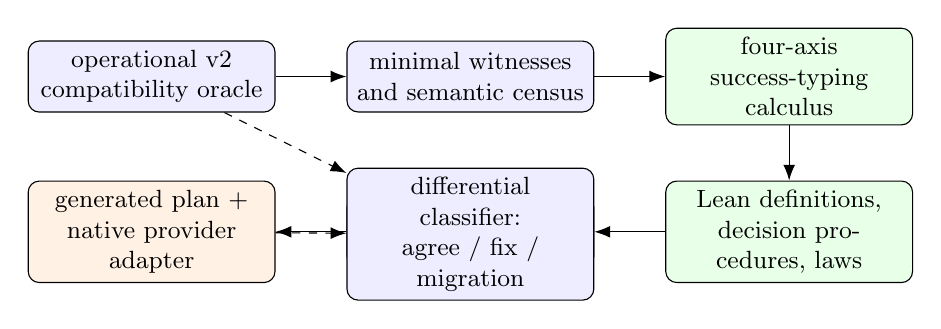
\begin{tikzpicture}[
  node distance=7mm and 9mm,
  box/.style={draw, rounded corners, align=center, minimum height=9mm,
              text width=29mm, font=\small},
  live/.style={box, fill=blue!7},
  proof/.style={box, fill=green!9},
  exec/.style={box, fill=orange!10},
  every edge/.style={draw, -{Latex[length=2mm]}}
]
\node[live] (oracle) {operational v2\\compatibility oracle};
\node[live, right=of oracle] (census) {minimal witnesses\\and semantic census};
\node[proof, right=of census] (axes) {four-axis\\success-typing calculus};
\node[proof, below=of axes] (lean) {Lean definitions,\\decision procedures, laws};
\node[exec, left=of lean] (langdef) {ordered v3\\LanguageDef rules};
\node[exec, left=of langdef] (native) {generated plan $+$\\native provider adapter};
\node[live, below=of census] (diff) {differential classifier:\\agree / fix / migration};
\path (oracle) edge (census)
      (census) edge (axes)
      (axes) edge (lean)
      (lean) edge (langdef)
      (langdef) edge (native)
      (oracle) edge[dashed] (diff)
      (native) edge[dashed] (diff);
\end{tikzpicture}
\caption{Distillation, not cloning.  The compatibility checker supplies
observations; the v3 implementation is generated from a factored calculus.
V2 is never used as a v3 fact interface: the two meet only at a compatibility
or differential boundary.}
\label{fig:petta-typecheck-distillation}
\end{figure}

The four axes are:

\begin{center}
\begin{tabular}{p{.19\linewidth}p{.34\linewidth}p{.37\linewidth}}
\toprule
Axis & Native object & Governing distinction \\
\midrule
Shape compatibility
  & directional consistency on primitive, list, product, union, arrow,
    alias, and nominal-newtype shapes
  & an actual union is universal; a required union is existential; unknown
    is compatible ignorance, not a proof of equality \\
Result cardinality
  & the grade order $\mathsf{det}\leq\mathsf{semidet}\leq\mathsf{nondet}$
    and grade sequencing
  & a deterministic promise cannot be discharged by a computation that may
    fail or branch; effect variables remain polymorphic \\
Stage evidence
  & held, evaluated, and compiled evidence, with an explicit grounding
    license
  & quoted code does not masquerade as its executed value; grounding requires
    compiled-stage evidence \\
Open-world knowledge
  & unknown, empty, or positively typed result evidence, plus selector facts
  & ignorance yields \emph{undetermined}; exhaustion yields
    \emph{incomplete}; only a replayable conflict yields \emph{refuted} \\
\bottomrule
\end{tabular}
\end{center}

The first row explains an initially surprising polarity law.  If a value is
known to be a \code{Number}, a requirement of
\code{(| Number String)} is satisfied by one member.  If the value itself may
be either \code{Number} or \code{String}, a \code{Number}-only requirement is
unsafe because \emph{every} actual alternative must be admissible.  Thus
consistency is deliberately directional and, in the presence of unknown
information, deliberately non-transitive.

\paragraph{A source-level example.}
The following selector is total on proper lists.  The identity
\code{let*} and its administrative alias must preserve both the
\code{List Number} shape and the deterministic grade:

\begin{lstlisting}
(: keep-number (-[det]-> Number Number))
(= (keep-number $x) $x)

(: select-list
   (-[$effect]-> (List Number)
                 (-[$effect]-> Number Number)
                 Number))
(= (select-list () $k) ($k 0))
(= (select-list (cons $head $tail) $k) ($k $head))

(: caller (-[det]-> Number))
(= (caller)
   (select-list
      (let* (($source (cons 1 ()))
             ($items  $source))
        $items)
      keep-number))
\end{lstlisting}

v3 accepts \code{caller}: lexical names elaborate to de Bruijn indices,
alias resolution transports the original runtime evidence, and the selector
consumes the positive proper-list fact.  Replacing
\code{(cons 1 ())} by \code{1} is the negative mirror: the alias still
transports evidence exactly, so the call is rejected at the named shape
boundary rather than accidentally acquiring a list fact.  Replacing the
producer by a nondeterministic superposition of Booleans similarly preserves
shape but fails a deterministic cardinality promise.  These paired examples
ensure that ``transport'' means preservation, not widening.

Stage evidence supplies a second compact example:

\begin{lstlisting}
(: Count (Newtype Number))

(: held-count (-[det]-> Count))
(= (held-count) (quote (brand Count 1)))      ; rejected: held code

(: evaluated-count (-[det]-> Count))
(= (evaluated-count)
   (eval (quote (brand Count 1))))            ; accepted: reactivated
\end{lstlisting}

Quotation preserves latent evidence but does not expose it as runtime typing
evidence.  Only the explicit \code{eval} transition reactivates it.  Native
v3 therefore rejects \code{held-count} and establishes
\code{evaluated-count}; the latter is recorded as a named refinement and
continues to follow v2 until that refinement is explicitly promoted.  This is
why the calculus can make the historical source-grounding defect
unrepresentable: source shape alone cannot construct a grounding license.

\paragraph{Runtime authority and status.}
The executable checker sees program state through exactly five
revision-keyed fact interfaces:
\begin{lstlisting}
EnvDeclared              EnvDeclaredList
EnvNonNewtype            KnownExpressionEffect
KnownExpressionResultType
\end{lstlisting}
They derive facts from the live \PeTTa{} program; they do not call v2 to
manufacture v3 answers.

\begin{figure}[ht]
\centering
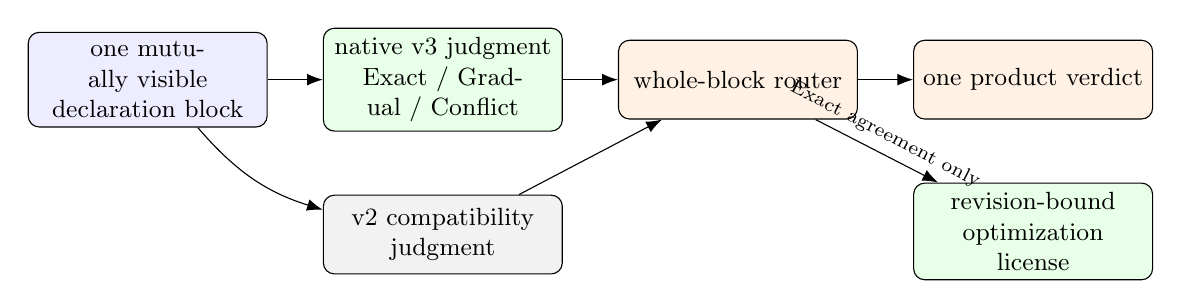
\begin{tikzpicture}[
  node distance=8mm and 7mm,
  box/.style={draw, rounded corners, align=center, minimum height=10mm,
              text width=28mm, font=\small},
  every edge/.style={draw, -{Latex[length=2mm]}}
]
\node[box, fill=blue!7] (block) {one mutually visible\\declaration block};
\node[box, fill=green!9, right=of block] (native) {native v3 judgment\\Exact / Gradual / Conflict};
\node[box, fill=gray!10, below=of native] (legacy) {v2 compatibility\\judgment};
\node[box, fill=orange!10, right=of native] (router) {whole-block router};
\node[box, fill=orange!10, right=of router] (verdict) {one product verdict};
\node[box, fill=green!9, below=of verdict] (license) {revision-bound\\optimization license};
\path (block) edge (native)
      (block) edge[bend right=16] (legacy)
      (native) edge (router)
      (legacy) edge (router)
      (router) edge (verdict)
      (router) edge node[above,sloped,font=\scriptsize]{Exact agreement only} (license);
\end{tikzpicture}
\caption{The KISS compatibility waist.  Routing is per complete block, so a
recursive definition group never mixes authorities.  A gradual result,
conflict, unpromoted refinement, or legacy route cannot mint an optimization
license.}
\label{fig:petta-typecheck-authority}
\end{figure}

At the same 2026-08-14 snapshot, the Lean core contains the executable
sound-and-complete consistency decision procedure, the cardinality and stage
algebras, lexical evidence transport, products, aliases, rational-tree
boundedness, and the Exact/Gradual/Conflict seam, with no holes.  Its ordered
LanguageDef mirror contains 149 rules (134 core and 15 seam rules) and passes
three order/multiplicity mutation canaries.  The isolated native harness
passes 353/353 checks, including product canaries that distinguish exact
agreement from rejection and gradual fallback.  All 51 census-selected
source candidates are executable end to end.  In particular, v3 derives
undeclared result/effect
contracts from the revision-keyed live equation set, retains heterogeneous
results as precise unions, and distinguishes proved concrete selection from
unresolved open patterns.

The complete 389-case differential classifies 214 cases as native agreement,
four as named refinements, and 171 as whole-block legacy-v2, with zero
unclassified, incomplete, or faulted cases.  Current-upstream PeTTaChainer
qualification passes all three representative programs after small,
semantics-preserving migrations that replace effect-polymorphic traversal
helpers with explicit typed recursion.  The no-typecheck profile and v3 both
match the PeTTa reference on those programs.

The optional v3 profile is not yet free.  Three matched runs on the same
materialized programs give the following medians; v3 includes both admission
and ordinary execution:

\begin{center}
\begin{tabular}{lrrrr}
\toprule
Program & no typing & typecheck-v3 & wall ratio & RSS ratio \\
\midrule
\code{deductionrevision} & 1.49\,s & 4.59\,s & 3.08$\times$ & 2.41$\times$ \\
\code{flyingraven}       & 6.07\,s & 12.10\,s & 1.99$\times$ & 1.59$\times$ \\
\code{raveninduction}    & 1.97\,s & 5.26\,s & 2.67$\times$ & 1.98$\times$ \\
\bottomrule
\end{tabular}
\end{center}

This is an integration baseline, not an optimization claim.  Typed fast paths
remain disabled until an exact, current license is consumed at an appropriate
construction boundary.  These denominators are intentionally separate:
operational compatibility, theory/LanguageDef parity, native coverage,
product migration, and execution cost are different claims.

\subsection{Oracle Conformance}
\label{sec:conformance}

For \code{he-compat}, upstream \HE{}~v0.2.10 is the sole oracle, and
the harness is a fail-by-default gate, not a green-manufacturing
report.  Comparison is by \emph{result-bag equality}---multisets of
parsed results, never byte-equality of output text---so formatting
differences cannot masquerade as semantic agreement, and duplicate
results (which are semantically real in MeTTa) are counted.

\begin{description}
\item[Current \HE{} I/O semantic gate.] The per-build oracle gate
  (\code{make test-he-compat-semantic-suite}) replays 23 curated
  \HE{} I/O fixtures against the upstream \HE{}~v0.2.10 baseline.  The
  July~2 receipt reports 23/23 \CeTTa{} passes, 0 failures, and a
  passing baseline check.  Six of those fixtures are core anchors into
  the Lean-side HE I/O conformance file.  This is the current
  conformance claim used by the paper.
\item[Archived catalog material.] Earlier generated rule-capacity and
  broad-corpus catalogs remain useful triage artifacts, but they are not
  treated as current paper evidence unless their driver emits the claimed
  counts on the audited tree.  In particular, this revision does not
  carry a 24-capacity maturity table or a broad-corpus count as a live
  conformance result.
\item[Adjudicated divergences.] Where \CeTTa{} deliberately diverges
  from upstream, each case carries independent grounds.  Three
  examples: upstream's post-0.2.10 \code{function}/\code{NoReturn}
  behavior contradicts its own written specification (a deliberate
  loop fix that left the document stale); upstream's \code{get-doc}
  errors on \HE{}'s own documentation example (an arity regression);
  and the user-visible result of top-level \code{eval} on a
  non-reducible term is genuinely under-determined by the
  specification---both engines deviate from the literal
  instruction-layer reading, in opposite directions.
\end{description}

The conformance material carries an explicit
\code{no\_runtime\_trace\_or\_certificate\_surface} flag, enforced by
the suite: conformance is \emph{testing}, and the specification is
what gets \emph{proven about} in Lean.  \CeTTa{} does not emit
execution traces or certificates, and a per-run check is never
presented as a proof.

\subsection{Evaluator Bug Classes the Campaign Exposed}
\label{sec:bugclasses}

Three bug classes were found and fixed, all instructive.

\paragraph{The Empty algebra.}  When overlapping equations yield a
branch that reduces to \code{Empty}, two dual defects appeared: the
surviving sibling branch was returned without being re-driven to
applicative normal form (violating the spec's applicative order), and
in other shapes \code{Empty} itself leaked into the visible result bag
(the spec is explicit that \code{Empty} ``is not returned among other
results'').  The fix treats the evaluator's outcome set as an algebra
with \code{Empty} as its absorbing zero and re-drives surviving
branches independently of their siblings.  In modal terms
(Section~\ref{sec:modal}): the successor algebra must satisfy
$\Diamond\bot = \bot$.

\paragraph{The one-step congruence bug.}  The reflective one-step
layer reported \code{(+ 1 (+ 2 3))} as a \emph{normal form}: the
one-step relation lacked argument congruence (stepping a reducible
argument when the head cannot fire), while the big-step evaluator had
it.  Because the one-step relation and the evaluator were separately
hand-maintained C branch sets, the gap replicated identically across
three development branches and was invisible to every test that only
exercised head-reducible terms.  The bug was diagnosed through the
modal layer itself ($\Box\bot$ holding on a reducible term), fixed
as deterministic left-to-right congruence matching the evaluator's
applicative order---and is the direct motivation for the rule-pack
weld in Section~\ref{sec:langdefpack}.

\paragraph{The switch/switch-minimal conflation.}  Upstream \HE{}
types \code{switch} as \code{(-> \%Undefined\% Expression
\%Undefined\%)}---the scrutinee is \emph{evaluated} before
matching---while \code{switch-minimal} is \code{(-> Atom Expression
Atom)}, matching the raw scrutinee structurally.  \CeTTa{} routed both
spellings through one structural handler, so
\code{(switch (+ 1 2) ((3 three) ((\$x \$y) (got \$x \$y))))} returned
\code{(got 1 2)} where upstream returns \code{three}.  The defect was
exposed not by testing but by the certification campaign
(Section~\ref{sec:rulecert}): modeling the rules in Lean forced a
precise reading of the two upstream type contracts, and an oracle
probe confirmed the divergence.  The fix splits the rule into
\code{HES\_Switch} (evaluated scrutinee) and \code{HES\_SwitchMinimal}
(structural), with a distinguishing witness pair pinned in the test
suite.

\paragraph{A representative conformance probe.}
The defect classes above are locked by gates rather than by a standing
program suite (standing suites tax every future run; the classes are
the durable artifact).  One representative probe is worth stating
because its \emph{correct} answer is doubly instructive:

\begin{verbatim}
(= (same $x $x) hit)
!(same a a)   ; [hit]
!(same a b)   ; [(same a b)]  -- inert, NOT hit, NOT empty
\end{verbatim}

\noindent
A nonlinear pattern constrains both positions to be equal, so
positional pattern compilation without an equality check answers
\code{hit} --- and an engine grounded in a failure-driven host answers
with an empty bag --- while the specified behaviour is that the
unmatched call remains \emph{uninterpreted}.  \CeTTa{}'s eager and lazy
lanes and upstream \HE{} agree on this and on the sibling probes for
grounded-argument strictness, duplicate multiplicity, view
invalidation, and strict equality; engines with different declared
semantics (\PeTTa{}'s Prolog grounding, set-carrier stores) simply
answer as their own specifications say, which is what declared
contracts are for.

\subsection{The Reflective Modal Layer}
\label{sec:modal}

The library \code{lts} (generic, step-parameterized) and
\code{lts:he} (bound to the \HE{} evaluator's one-step relation) reflect the
one-step reduction relation into MeTTa as data:

\begin{itemize}
\item \code{lts:he:transitions} emits the one-step successor set
  of an atom as quoted states (zero results on quiescent atoms);
  \code{lts:he:trace-2} enumerates two-step traces.
\item \code{lts:he:is-normal-form} is exactly $\Box\bot$ (every
  successor satisfies falsity, i.e.\ no successor exists);
  \code{lts:he:is-can-step} is $\Diamond\top$.
\item \code{lts:he:box}~$\phi$ and \code{lts:he:diamond}~$\phi$
  generalize these to arbitrary unary predicates: $\Box\phi$ holds
  when every one-step successor satisfies $\phi$ (vacuously at normal
  forms), $\Diamond\phi$ when some successor does.
\end{itemize}

The De~Morgan law $\Box\phi = \lnot\Diamond\lnot\phi$ is installed as
a runtime self-test; it is the executable mirror of the Galois
connection proven once and for all in the Mettapedia OSLF framework,
where $\mathrm{LanguageDef}\to\mathrm{RewriteSystem}\to
\mathrm{ReductionSpan}\to(\Diamond,\Box)$ is derived generically and
\code{langGalois} establishes the adjunction.  Native behavioral types
in the sense of Native Type Theory arise as predicates over exactly
this reduction span; the runtime implementation and the Lean derivation
describe the same object at two levels.

Multiplicity discipline: \code{transitions} preserves the result
\emph{bag} (duplicate successors are semantically real), while the
modal predicates quotient to reachability.  Evaluation and conformance
compare bags; $\Diamond/\Box$ use support.  Result sets are never
deduplicated for speed.

\subsection{The Small-Step Rule Table}
\label{sec:langdefpack}

The congruence bug demonstrated the structural disease: reduction
rules as anonymous, duplicated C branches are invisible, unremovable,
and untestable-by-absence.  The cure is to make the rule set a
\emph{named, reflectable object} the evaluator provably depends on.

Three granularity strata are kept distinct.  \emph{HEFine} is the Lean
\code{mettaHE} instruction machine (59 rules over interpreter states;
the proof reference).  \emph{HE small-step} is the coarse user-visible
one-step relation---one observable source rewrite, e.g.\
\code{(+ 1 (+ 2 3))} $\to$ \code{(+ 1 5)}---which is what the
\code{lts} layer exposes.  \emph{HEBigStep} is full evaluation.  The
table encodes the small-step relation; its relationship to the fine machine is a
collapse/simulation with explicit provenance links (each coarse rule
names the fine rules that justify it), never a label identity.

The runtime object, \code{CettaLangDefPack}, carries: language,
profile, and granularity identifiers; a schema version; a source
digest over the canonical rule-descriptor text; the rule table; a
disabled-rule mask populated from the
\code{CETTA\_LANGDEF\_DISABLED\_RULES} environment variable; and a
\emph{per-rule claim level} recording the strongest evidence behind
each rule (Section~\ref{sec:rulecert}).  Ten rule classes are live and
gate the \emph{only} implementations of their behavior in the one-step
subsystem: grounded dispatch, leftmost expression congruence, equation
match, \code{eval}, \code{chain}, \code{let}, \code{let*},
\code{case}, \code{switch}, and \code{switch-minimal} (the last two
split per their distinct upstream contracts,
Section~\ref{sec:bugclasses}).  Quote/return and empty/error
quiescence are structural rows: accounted in the table with written
reasons, but not gateable, since disabling them would make the
semantics incoherent rather than smaller.  Each row carries a
provenance string naming the fine-machine rules that justify it.  The
pack is reflected into MeTTa by \code{lts:he:step-rules}.

The load-bearing test is \emph{anti-decorative}: a dedicated lane
re-runs the witness suite with each live rule disabled and
\emph{requires} the witnesses to fail (the successor set must go
empty; normal-form must flip)---baseline plus ten rule-removal
failures confirmed.  If the witnesses still passed with a rule
removed, a duplicate hidden code path would exist---precisely the
disease that produced the congruence bug.  A disabled special form
goes \emph{inert} (its head stays uninterpreted; congruence still
applies), per the principle that unknown symbols are data, never
errors.  The lane fails closed in both directions and runs on both the
default and MORK-bridge builds.

Claim levels are deliberately \emph{excluded} from the digest: the
digest fingerprints rule \emph{content} (names, profiles, provenance,
schema), while claims are \emph{evidence about} that content.
Upgrading a rule's certification therefore must not---and verifiably
does not---move the semantic object: the digest
(\code{fnv1a64:12eec5b655a75904} at the time of writing) stayed fixed
across every claim flip.  The pack is, by design, a hand-authored
object kept honest by the removal lane and the digest; we deliberately
parked an earlier plan to generate specialized C from the rule source,
because the weld's value lies in the named semantic object and its
fail-closed tests, and code generation is machinery the certification
program does not need.

\subsection{Lean Certification of the Rule Table}
\label{sec:rulecert}

Each per-rule claim takes one of three values, in increasing strength:
\emph{bag-tested-adequate} (the rule's behavior matches the legacy
path and oracle bags on the witness corpus),
\emph{rule-sound-on-fragment} (a compiled, sorry-free Lean theorem
proves the rule absorbed by the official declarative semantics on an
explicitly characterized fragment), and \emph{rule-sound} (the same,
unconditionally).  A claim flips only when the compiled theorem
exists, so the reflective layer can never overclaim.  The
certification route is \emph{absorption}: for each coarse rule, a
theorem that whenever the rule relates $a \to a'$, the official
declarative judgment of the Mettapedia \HE{} formalization
(\code{MettaCall}, \code{MinimalStep}, or \code{EvalAtom}) already
relates the same atoms.  At the time of writing five of the ten live
rules carry certification:

\begin{center}\footnotesize
\begin{tabular}{lll}
\toprule
rule & claim & Lean witness \\
\midrule
\code{HES\_GroundedDispatch} & rule-sound &
  \code{mettaCall\_absorbs\_grounded\_dispatch} \\
\code{HES\_EquationMatch} & rule-sound &
  \code{mettaCall\_absorbs\_equation\_match} \\
\code{HES\_Eval} & rule-sound &
  \code{minimalStep\_absorbs\_eval} \\
\code{HES\_Chain} & rule-sound-on-fragment &
  \code{minimalStep\_absorbs\_chain\_source}/\code{\_subst} \\
\code{HES\_LeftmostExprCongruence} & rule-sound-on-fragment &
  \code{evalAtom\_absorbs\_congruence\_frag} \\
\code{HES\_Let}, \code{LetStar}, \code{Case}, & bag-tested-adequate &
  in progress \\
\quad\code{Switch}, \code{SwitchMinimal} & & \\
\bottomrule
\end{tabular}
\end{center}

The certified fragment for the congruence and chain rules is
characterized positively: untyped constructor-headed expressions with
quiescent spectator arguments and a grounded-dispatch or
equation-match redex.  Its supporting theory is a short ladder of
compiled lemmas: a quiescence domain on which atoms officially
self-evaluate, uniqueness of that self-evaluation, transport of
official evaluation across a single changed argument, and absorption
of inner fragment steps---about which the honest surprises accumulated
(e.g.\ a bare \code{Error} \emph{symbol} at tuple head becomes
error-shaped, so the fragment must exclude it explicitly).

The five remaining rules are upstream \emph{stdlib sugar}: their
one-step behavior is the upstream definition of \code{let},
\code{let*}, \code{case}, \code{switch}, and \code{switch-minimal} as
\code{unify}/\code{chain} programs.  Certifying them required a
\emph{matcher bridge}: relating the public equation-query API to the
official \code{matchAtoms}/\code{mergeBindings} semantics.  The key
insight from this development stage was that the real seam was \emph{not} merely a
direct one-way-to-two-way matcher comparison.  The public \HE{} query
API had historically routed equation lookup through the simplified
\code{simpleMatch} path, while the faithful two-sided matcher already
existed separately.  We therefore split the bridge into three explicit
layers.

First, \code{DeclMatchSpec.lean} states the author's
\code{match\_atoms} semantics declaratively and proves the executable
\code{matchAtoms} helper sound and complete against it
(\code{matchAtoms\_sound}, \code{matchAtoms\_complete}).  Second,
\code{DeclMergeSpec.lean} does the same for
\code{merge\_bindings}/\code{add\_var\_binding}/\code{add\_var\_equality},
proving \code{mergeBindings\_sound} and
\code{mergeBindings\_complete}.  Third,
\code{QueryInterfaceAgreement.lean} proves a bounded adequacy theorem for
the \emph{public} query interface:
\code{queryEquations\_ground\_two\_way\_adequate} and its
\code{queryEquationsAgainstVisible}-companion show that, on the
ground-query fragment and under the explicit freshening adequacy
hypothesis \code{EquationFresheningAdequate}, the repaired
\code{matchAtoms}/\code{mergeBindings} API and the legacy
\code{simpleMatch}-based scan agree in both directions up to replay
fuel.

The earlier singleton-seed factorization theorem remains one ingredient
inside this story, but it is no longer the whole story.  The decisive
insight is the G3/G3b split: equality-threading becomes observable only
when the queried atom itself still contains variables, because that is
the point at which \code{Bindings.resolve}/\code{Bindings.apply} must
honor equalities rather than plain assignments.  We therefore bank the
ground-query adequacy result as the honest current certification
API, and carry the variable-bearing query case as an explicit next
obligation rather than silently pretending the legacy API was already
faithful.

%% ────────────────────────────────────────────────────────────────────
\section{Verified \HE{}$\leftrightarrow$\PeTTa{} Translation}

\subsection{Bidirectional Translator}

A bidirectional translator converts between \HE{} and \PeTTa{} dialects.
It is implemented both as relational Prolog
(\code{he\_petta\_relational.pl}, with explicit freshness threading) and
as computable Lean functions (\code{translateHE}, \code{translatePeTTa}).

The translator handles 8 \HE{}$\to$\PeTTa{} rewrite rules
(\code{chain}$\to$\code{let}, \code{collapse-bind}$\to$\code{collapse},
\code{nop}$\to$\code{let~\$fresh~X~()}, etc.)\ and 5
\PeTTa{}$\to$\HE{} rules (\code{progn}$\to$nested \code{let},
\code{prog1}$\to$\code{let} with result capture, etc.).  All 437 real
\code{.metta} files parse and translate successfully.

\subsection{Sorry-Free Lean Proof}

The translation is backed by a \textbf{sorry-free, axiom-free} Lean
proof across two files totaling 4{,}979 lines and 102
definitions/theorems:

\begin{description}
\item[\code{HEPeTTaSound.lean}] (1{,}063 lines, 44 theorems.)
  Proves that \HE{}'s equation matching corresponds to \PeTTa{}'s
  \code{ruleApp} evaluation.  The key result:
  \begin{quote}
  \code{simpleMatch\_applyBindings\_comm}: if \HE{}'s
  \code{simpleMatch} succeeds on two \code{PureTranslatable} atoms,
  then applying the translated bindings via \code{heBindingsToOSLF} to
  the translated pattern recovers the translated target.
  \end{quote}
  This commutation property, combined with the existing
  \code{matchPattern\_applyBindings\_complete} from the OSLF framework,
  establishes that a \PeTTa{} \code{matchPattern} witness exists
  whenever \HE{}'s \code{simpleMatch} succeeds.

\item[\code{HEPeTTaTranslate.lean}] (3{,}916 lines, 58 theorems.)
  The executable translator with:
  \begin{itemize}
  \item \code{translateHE\_translatable}: translation preserves
    \code{Translatable} (output admits \code{atomToPattern}).
  \item \code{translateHE\_preserves\_pureTranslatable}: translation
    preserves the stronger \code{PureTranslatable} fragment.
  \item \code{translatePeTTa\_translatable}: same for the reverse
    direction.
  \item 9 \code{\#eval} tests matching Prolog output on concrete atoms.
  \item 6 \code{rfl} examples kernel-verified by Lean.
  \item Roundtrip idempotence examples (kernel-verified).
  \end{itemize}
\end{description}

%% ────────────────────────────────────────────────────────────────────
\section{Reflective $\rho$-calculus and eval-at-\textsc{comm}}
\label{sec:rhocalc}

Under \code{--lang rhocalc} the same runtime stops being a term rewriter and becomes a
concurrent process engine: its unit of work is not a rewrite but a \emph{reaction}, a
rendezvous between a sender and a receiver on a shared channel. This brings channels with
private names and genuine concurrency; and because the calculus is \emph{reflective}, a
received name can be \emph{run}, so a communication can itself be a computation. The MeTTa
library that exposes that last capability is \emph{rhometta}. We build up to it from the
pure calculus.

\subsection{The pure calculus}

The calculus is Meredith and Radestock's reflective higher-order
$\rho$-calculus~\cite{rho2005}. Its one reduction rule, \textsc{comm}, is a handshake
(Figure~\ref{fig:rho-comm}): a sender \code{x!(m)} on channel \code{x} beside a receiver
\code{for(y <- x)\{P\}} on that
same channel react; the message is consumed and the receiver resumes with \code{m}
substituted for its bound name \code{y}:
\[
  x!(m) \;\big|\; \mathsf{for}(y \leftarrow x)\{P\}
  \;\;\xrightarrow{\;\textsc{comm}\;}\;\; P[y := m].
\]

\begin{figure}[h]\centering
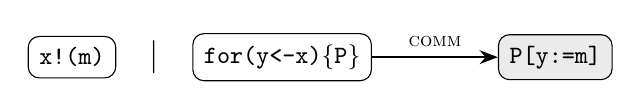
\begin{tikzpicture}[>=Stealth,
  box/.style={draw, rounded corners, align=center, inner sep=4pt,
    font=\small\ttfamily}]
  \node[box] (s) {x!(m)};
  \node (par) [right=3mm of s, font=\large] {$\mid$};
  \node[box] (r) [right=3mm of par] {for(y<-x)\{P\}};
  \node[box, fill=black!8] (out) [right=16mm of r] {P[y:=m]};
  \draw[->, thick] (r) -- node[above, font=\scriptsize\sffamily] {\textsc{comm}} (out);
\end{tikzpicture}
\caption{A reaction: a send and a matching receive on channel \code{x} rendezvous; the
  receiver continues with the message substituted in.}
\label{fig:rho-comm}
\end{figure}

The rest of the vocabulary is small. \code{0} is the inert process; \code{P | Q} runs
\code{P} and \code{Q} concurrently. Two reflection operators connect processes and names:
\code{@P} \emph{quotes} a process into a name, and \code{*x} \emph{drops} (runs) the process
a name quotes, with \code{*@P = P}. Channels are themselves quoted processes --- this is
what makes the calculus higher-order. \CeTTa{} implements exactly these six strict-core
constructors --- \code{rho:nil}, \code{rho:par}, \code{rho:send}, \code{rho:recv},
\code{rho:quote}, \code{rho:drop} --- with \textsc{comm} as the only reduction. A program is
reduced to quiescence by \code{cetta --lang rhocalc \textit{file}}, written either in a
MeTTa-style S-expression syntax (\code{.mrho}) or a Rholang-like syntax (\code{.rho}); the
runtime keeps a live index of sends and receive-sites, rebuilt after each reaction.  The
deterministic (canonical) scheduler selects the key-least successor by streaming candidate
keys against the best bound found so far instead of materializing and sorting the whole
frontier, which keeps single-step selection cheap on wide parallel terms.

\subsection{Reflection is enough}
\label{sec:rho-reflection}

A surprising amount follows from \textsc{comm} and quote/drop alone, with no further
primitives. Each item below is a standalone \code{--lang rhocalc} program.
\begin{itemize}
\item \emph{Name mobility.} A receive that drops its argument, placed beside a send carrying
  a quoted send, reduces to that inner send made live: a name has travelled across a channel
  and been activated.
\item \emph{Fresh names.} Quoting a distinct process yields a distinct name, so a receiver
  can mint and use a name it never mentioned syntactically.
\item \emph{Replicated input.} An input-guarded server can re-create its own listener:
  after serving a message it leaves a copy of the receiver in the residual, so the channel
  keeps serving. Persistent receive is \emph{derived}, not built in.
\item \emph{Recursion and divergence.} The same self-recreation, left ungated, runs without
  bound (the engine reports its reduction limit); recursion needs no dedicated operator.
\end{itemize}
Private channels and information hiding come along for free: a payload exchanged on a name
no other process holds is unobservable apart from whatever completion signal the protocol
chooses to publish.

The capstone is \emph{eval-at-\textsc{comm}}. Let the receiver do nothing but drop what it
receives:
\[
  \texttt{eval\_drop}(x,p)\;\equiv\;
  \underbrace{x!(@p)}_{\text{send the quoted program } p}\;\big|\;
  \underbrace{\mathsf{for}(y \leftarrow x)\{\,*y\,\}}_{\text{run whatever arrives}}.
\]
The \textsc{comm} delivers the name \code{@p}; the drop \code{*@p} runs \code{p}; the
process settles at the result of running \code{p}. A handshake has become an evaluation
step, and since \code{p} may itself evaluate to more process, a reaction can plant the next
reactions.

\subsection{Profiles}

A \emph{profile} names a variant of the reduction relation together with the grammar it
accepts. \code{strict-core} is the pure asynchronous spine above: it admits only the six core
constructors, and a non-core form is \emph{rejected} rather than left inert. The \code{cost}
profile accepts a richer resource-annotated dialect in which every reaction must be
\emph{funded} from purses located on its channel, and every run emits a causal receipt of
its spending (Section~\ref{sec:rho-cost}).

\subsection{Certified reduction}
\label{sec:rho-lean}

Does eval-at-\textsc{comm} report the result of running the payload, or could the machinery
quietly change the answer? We settle this in Lean. Run \code{eval\_drop(x,p)} to quiescence
and collect every outcome observable \emph{up to structural rearrangement} of the process;
that set is exactly the results a correct evaluation of \code{p} would produce, and the
statement refers only to what is observable, never to an internal ``this is the answer''
tag. The theorem \code{rhometta\_bridge\_scObserved} (in \code{RhometaReduction.lean})
equates the concrete quiescent run of \code{eval\_drop(x,p)} with
\code{RhometaSCObservedOutcomes} of the same process --- the outcomes visible up to
structural congruence --- with no result-certificate carried in the answer. Two ingredients
are load-bearing. First, a complete canonical-form normalizer \code{nfAtom}: two processes
are structurally congruent exactly when their normal forms coincide, which unblocks
inductions that otherwise stall on the symmetry and transitivity of congruence. Second, one
hygiene side condition \code{noBoundUnderQuote}: the communicated variable must not occur
under a quote, since a payload that hides a bound occurrence inside a quoted name defeats the
characterization (a concrete counterexample exhibits exactly that failure). The development
carries no \code{sorry}. A separate caveat on the trusted base: its conformance and DSL
fixtures use \code{native\_decide}; the bridge theorem's own module does not.

\subsection{rhometta: MeTTa at the reaction}

eval-at-\textsc{comm} becomes a way to program once the payload is a MeTTa term. The library
\code{lib/rhometta.metta} provides \code{rhometta:eval}, which defers a MeTTa term as the
payload to be run at \textsc{comm}; \code{rhometta:run}, which reduces a process to its
quiescent outcome set; and \code{rhometta:transitions}, which returns one-step successors. It
sits on \code{lib/rho.metta}, the strict-core constructor syntax, and delegates all
reduction to the engine. One consequence is central: when a deferred payload evaluates to
\emph{several} results, the \textsc{comm} forks --- one successor per result. Nondeterministic
computation becomes a branching reaction, and \code{rhometta:run} returns one residual per
branch (the \emph{may-set}).

\subsection{What reactions compute}

\paragraph{The minimal cell.} The smallest rhometta program is a single cell: a send carrying
a deferred term beside a receiver that drops (runs) it. \code{rhometta-eval-cell} sends
\code{(+ 2 3)} this way and the reaction leaves \code{5}; with a multi-result payload
\code{(superpose (a b c))} the \textsc{comm} forks into one branch per result, and
\code{rhometta:transitions} confirms the fork is a single reduction step with three
successors. Communication does computation, and result-multiplicity becomes branching.

\paragraph{A self-unfolding prover.} Seed a \emph{single} cell for a goal. Each \textsc{comm}
evaluates one backward-chaining step whose result is the cells for that goal's subgoals, so
\code{rhometta:run} keeps reducing and the reaction network unfolds itself into a proof tree.
Where a goal has several rules the payload has several results, so the \textsc{comm} forks:
\code{rhometta:run} returns one quiescent residual per complete proof tree
(Figure~\ref{fig:rho-tree}) --- two for the sample ``can I bake a cake?'' goal, while a
single-rule goal stays confluent at one.

\begin{figure}[h]\centering
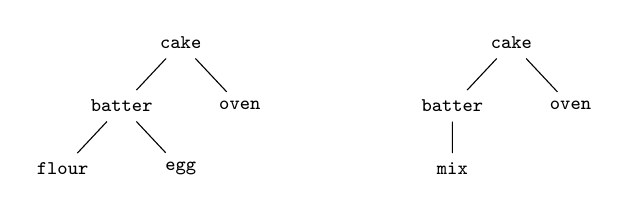
\begin{tikzpicture}[>=Stealth, level distance=8mm, sibling distance=15mm,
  every node/.style={font=\scriptsize\ttfamily}, edge from parent/.style={draw,-}]
  \begin{scope}
  \node {cake} child { node {batter} child { node {flour} } child { node {egg} } }
               child { node {oven} };
  \end{scope}
  \begin{scope}[xshift=42mm]
  \node {cake} child { node {batter} child { node {mix} } }
               child { node {oven} };
  \end{scope}
\end{tikzpicture}
\caption{The self-unfolding prover's may-set for ``cake'': two complete proof trees, one per
  rule for \code{batter}. The trees are not enumerated up front --- they are \emph{grown} by
  reactions whose payloads plant their children.}
\label{fig:rho-tree}
\end{figure}

\paragraph{Type inference as proof search.} A typing judgment \code{(: proof (HasType e t))}
is proved by reactions over typing rules, and the proof term is the derivation. In
\code{rhometta-type-inference}, an overloaded \code{plus} yields a genuine may-set --- an
\code{Int} and a \code{Float} typing of \code{(plus one one)} --- while \code{(plus x one)}
with \code{x : Int} prunes the \code{Float} branch at the unification join. Proof terms stay
pure, \code{(: (app pf pa pb) (HasType e t))} --- a typing is crisp, so no truth value is
attached. Each result is cross-checked differentially against a sequential
chainer over the same knowledge base, which derives the same proof-term skeletons.

\paragraph{A truth value that is earned.} Crisp proof terms are the right output for a typing,
but some judgments are genuinely probabilistic, and there a reaction can carry evidence rather
than certainty. In \code{rhometta-evidence-revision}, two agents each count their own
observations of ``ravens are black'' into an opinion --- a strength and a confidence ---
computed at \textsc{comm} by a deferred payload. The two agents share two observations, so
merging their opinions \emph{naively} double-counts the shared evidence and overstates the
confidence ($0.889$); an overlap-corrected revision discounts the shared stamps for the honest
value ($0.857$), at the same strength. The revision can run after the parallel fan-in, or
\emph{at} the final rendezvous itself. This is the one place a truth value belongs --- it is
counted from data, not attached by hand.

\paragraph{Composition.} These pieces compose: a further program runs an independent proof
search, an overlap-corrected evidence revision, and an attention-spreading step concurrently,
then rendezvouses their channel-gathered results into a single synthesis.

\subsection{Cost-accounted reactions}
\label{sec:rho-cost}

A reaction is the natural unit of metering: each \textsc{comm} is one indivisible piece of
work. The \code{cost} profile makes that intuition operational --- and it does so with money
rather than a stopwatch. Processes are \emph{signed}, channels carry \emph{purses} of
tokens, a reaction fires \emph{only if it is paid for}, and what a run returns is not a
number but a \emph{receipt}: a causal, auditable record of every spend. The profile is the
executable part of the programme to equip the $\rho$-calculus with compositional resource
accounting~\cite{costendofunctor,rhocost-companion}. Its design commitments are locality of
funding, causality from consumption, and an explicit separation between exact authority
receipts and lossy numerical valuations.

\paragraph{Purses and funded reactions.} In the \code{.rho} syntax, \code{\{P\}alice} is
the process \code{P} signed by \code{alice}, and \code{purse pay \{alice : ()\}} is a store
on channel \code{pay} holding one token signed by \code{alice}. The funding rule is
\emph{located}: a \textsc{comm} on \code{pay} consumes one token per participating endpoint
signature, and those tokens must be found in purses \emph{on \code{pay} itself}. There is no
ambient bank account, and raw process data never funds anything. The smallest funded program
has two signed endpoints and two purses
(\href{https://github.com/zariuq/CeTTa/blob/e23de3043462d80e27f9c9009bd0f1b955ed140c/tests/rhocalc_cost_run/split_tokens_basic.rho}{\code{tests/rhocalc\_cost\_run/split\_tokens\_basic.rho}}):

\begin{lstlisting}
{for ($m <- pay) {{0}cont}}alice | {pay!({0}payload)}bob
  | purse pay {alice : ()} | purse pay {bob : ()}
\end{lstlisting}

\noindent
which reduces to \code{purse pay \{()\} | purse pay \{()\} | \{0\}cont}: each signature paid
for its own endpoint, and the two purses are left empty beside the continuation. Now delete
\code{bob}'s purse
(\href{https://github.com/zariuq/CeTTa/blob/e23de3043462d80e27f9c9009bd0f1b955ed140c/tests/rhocalc_cost_run/missing_token_quiescent.rho}{\code{missing\_token\_quiescent.rho}}) and
the program is \emph{quiescent with the send and receive still facing each other}: the
reaction is not slowed, it is \emph{disabled}. This is the first thing to internalize about
the profile --- cost is not an observer bolted onto the side; an unfunded reaction cannot
fire. Because channels are quoted processes, a purse's location follows the calculus's own
name equivalence rather than spelling: a purse on \code{@\{*pay\}} funds a reaction on
\code{pay}, since the two names denote the same channel
(\href{https://github.com/zariuq/CeTTa/blob/e23de3043462d80e27f9c9009bd0f1b955ed140c/tests/rhocalc_cost_run/name_equivalence_quote_drop.rho}{\code{name\_equivalence\_quote\_drop.rho}}) ---
aliases of a channel are the same account.

\paragraph{Receipts are causal records, not counters.} A single number would forget who
paid, what was consumed, and what depended on what --- and its intermediate readings would
depend on which interleaving the scheduler happened to choose. Instead, every reaction emits
an event record with four fields: a fresh event identifier; a \emph{cause list} --- the
identifiers of the events that produced the exact occurrences this event consumed, with
repetitions kept (consuming two outputs of event $0$ yields the cause list \code{(0 0)}); a
nonempty list of \emph{funding} records naming the purse location and head signature of each
token spent; and the consumed signature itself. The two-reaction chain below (the first case
of
\href{https://github.com/zariuq/CeTTa/blob/e23de3043462d80e27f9c9009bd0f1b955ed140c/tests/test_lts_rho_cost_causal_trace.metta}{\code{tests/test\_lts\_rho\_cost\_causal\_trace.metta}})
shows the shape --- event $1$ consumes both a continuation and a purse tail produced by
event $0$, so its cause list holds two arcs to $0$:

\begin{lstlisting}
(lts:rho:cost:receipt
  ((lts:rho:cost:event 0 ()
     ((lts:rho:cost:funding chain spend)) spend)
   (lts:rho:cost:event 1 (0 0)
     ((lts:rho:cost:funding chain spend)) spend))
  (rho:cost:par
    (rho:cost:purse chain rho:cost:stack-empty)
    (rho:cost:signed rho:nil done)))
\end{lstlisting}

The algebraic reading is the load-bearing one. A receipt is a \emph{located, measured
pomset} of spend events: a partially ordered multiset whose order is generated purely by
consumption --- event $e'$ follows $e$ exactly when $e'$ consumed something $e$ produced.
The engine's emission order is one linearization of that partial order.  Any
permutation of one fixed compatible matching yields the same target and receipt
bag; the emitted sequence linearizes that matching's causal order.  Alternative
endpoint or funding matchings remain distinct branches.  The Lean theorem
\code{boundedBudgetedCausalPrefix\_emission\_linearizes} confirms that a budgeted
prefix's emitted sequence linearizes its causal order. Locations make purses \emph{fibers} over channels: funding
never crosses a channel, and each per-location account is conserved
(\code{CostPath.per\_location\_restriction\_account\_conservation}). Finally, the receipt
itself carries no notion of ``the cost'': costs are \emph{valuations} --- monoid-valued maps
out of the receipt (total spend, per-signature spend, critical-path depth) --- so the
receipt is the free object and each accounting policy is a homomorphism out of it, with the
lawful combination rules derived rather than posited, in the sense of Knuth and Skilling's
measure-assignment axioms~\cite{knuthskilling}. Event identifiers are deliberately
polymorphic in the same spirit: a local counter suffices in one process, and a hash-chained
identifier can replace it at trust boundaries with the receipt algebra unchanged.

\paragraph{Honest budgets.} Everything above is unbounded by default:
\code{lts:rho:cost:steps} and \code{lts:rho:cost:causal-trace} enumerate exactly and never
truncate silently. Bounded execution is strictly opt-in through
\code{lts:rho:cost:causal-prefix}, which takes two separate allowances --- reaction fuel and
exact-cover search work --- and returns a receipt together with a status that never lies:
\code{quiescent} only after exhaustive search \emph{proves} the residual has no funded
successor; \code{fuel-exhausted} when the firing allowance ends first;
\code{search-exhausted} when cover search stops before finding a successor \emph{or proving
absence}. Search exhaustion is never reported as quiescence: an out-of-fuel machine says ``I
ran out,'' never ``there was nothing there.'' The distinction has teeth because funding
search is a genuine exact-cover problem. A send whose signature product multiplies ten
\code{coin}s, beside twenty unit purses on the same channel, admits
$\binom{20}{10}=184{,}756$ distinct covers
(\href{https://github.com/zariuq/CeTTa/blob/e23de3043462d80e27f9c9009bd0f1b955ed140c/tests/test_lts_rho_cost_search_budget.metta}{\code{tests/test\_lts\_rho\_cost\_search\_budget.metta}}):

\begin{lstlisting}
; Zero reduction fuel performs no exact-cover search, even when
; the latent cover family has C(20,10) members.
!(assertEqualToResult
  (test:prefix-status
    (lts:rho:cost:causal-prefix 0 0 (test:large-cover-state)))
  (lts:rho:cost:fuel-exhausted))

; The first exact occurrence cover is yielded without
; materializing the other 184,755 covers.
\end{lstlisting}

\noindent
At fuel $0$ the machine performs no search at all; with a small search allowance it yields
the first cover lazily; and the unlimited frontier remains available and exact --- all
$184{,}756$ successors, measured at about $11$\,s --- combinatorial by design and by
request, never by accident. A budget-monotonicity gate (59 paired runs at increasing
allowances) checks that raising an allowance never flips a determinate verdict and never
removes a receipt event: more fuel can only extend what is known.

\paragraph{Certified correspondence.} The formal side lives in the \code{Cost/}
theory in the Mettapedia repository: cost steps, paths, receipts, valuations,
conservation laws, and a budgeted executor, proven equal to one another where they meet.
The capstone \code{BudgetedPrefixPathRefinement} states that every budgeted machine run
produces a prefix of the occurrence-bearing Lean executable \code{CostPath}, with
the same receipt and the correct status,
and its corollaries pin each verdict separately: sufficient allowances yield an actual
path; exhaustive candidate failure --- unlike bounded exhaustion --- certifies quiescence;
zero fuel and zero search-work report their own exhaustion and make no negative claim. The
machine frontier is proven sound and complete up to structural equivalence
(\code{costStep\_sound\_runtime},
\code{costStep\_complete\_runtime\_up\_to\_struct}); these are the separate
one-step correspondences with the declarative \code{CostStep} relation.
The compositional theorem
\code{budgetedCausalPrefix\_exists\_rhoLanguageDefRewritePath} closes the
corresponding path square for the Lean executor: every publicly admitted
budgeted run yields an occurrence-bearing runtime path, a declarative funded
trace, and a rewrite path in the pure GSLT mechanically derived from
\code{rhoCalc}, with exactly one pure step per runtime firing.

The pure-rho boundary is theorem-backed as well.  The authored rho
\code{LanguageDef} supplies the strict syntax and primitive COMM presentation;
its compiled matcher, normalization, substitution, and supported COMM contracta
are proved to agree with the independently established semantic development.
The pure GSLT used for erasure is itself derived from that authored declaration;
full equivalence of its complete contextual relation with the independently
established relation remains a named theorem obligation.  On the derived
binder-safe fragment, initialization and funded reduction preserve scope; each
declarative \code{CostStep} erases to one derived pure \textsc{comm}, and each
declarative funded or executable path erases to a derived rho rewrite path whose
length is exactly its ordered demand-receipt length.  The equivalence used here
is pure structural congruence: no executable free-Drop step is admitted.  The
canonical configuration erasure is defined by quotient lifting rather than by
a noncomputable representative choice.  The pure-erasure binder-safety judgment
covers exactly syntax observable by pure erasure.  The separate public
runtime-scope check validates every raw field, including purse locations, and is
proved to imply the erasure-domain judgment.
A rerunnable Lean audit prints the axioms of the exported results; they use only Lean's
standard quotient and classical infrastructure, with no project axiom and no unfinished
proof.

On the compiled side, 146 sequential/threaded prefix cases agree, and 308 compiled-C
receipts replay as Lean derivations while two altered receipts are rejected.  The complete
runtime suite passes in the ordinary, thread-sanitized, and address/undefined-behavior
sanitized builds.  The differential harness
(\href{https://github.com/zariuq/CeTTa/blob/e23de3043462d80e27f9c9009bd0f1b955ed140c/scripts/rhocalc_cost_differential.py}{\code{scripts/rhocalc\_cost\_differential.py}})
drives the same terms through the C engine and the Lean executor, including fuel-$0$ and
fuel-$1$ boundary cases, with an out-of-fragment case correctly rejected. This remains
bounded differential evidence about the compiled engine, not a universal theorem about C.

\paragraph{Parallel funded execution.} Compatible reactions execute in OS threads in
waves.  Before a worker can fire, it atomically claims the exact endpoint occurrences and
the exact funding-cover occurrences in a fixed resource order; a wave admits only pairwise
disjoint claims.  The sequential semantics therefore remains the reference, while the
threaded implementation is tested as a legal parallel refinement: both threaded CLI modes,
six contention and disjointness stress families, and the sequential/threaded prefix gate
exercise same-channel disjoint reactions, competing funding covers, duplicate-looking
occurrences, and causal receipt linearization.  Receipt emission is an \emph{optional
observer} on this path: operational components are plain terms, causal provenance rides in a
parallel producer vector, and a scripted transparency gate checks that a state-only run and a
receipt-observed run consume identical resources and reach the same residual.  These gates,
together with thread and memory sanitizers, are implementation evidence; the Lean step/path
theorem above supplies the declarative semantic boundary.

At the modeled parallel boundary, a list of enabled runtime candidates whose
complete endpoint-and-funding source-index family is globally duplicate-free
lifts to a \code{SelectedRuntimeWave}.  Its witnessed source partition
constructs an exact \code{CostMatching}, and every permutation of that fixed
matching serializes as an ordinary declarative cost trace.  This discharges the
runtime-model wave-to-matching square under the occurrence-claim postcondition;
the compiled-C correspondence remains the bounded differential, receipt-replay,
and sanitizer evidence stated above rather than a universal theorem about C.

\paragraph{A strict source presentation and the corrected algebra.} The profile implements
funded rho and no Datalog architecture.  Its strict syntax and primitive \textsc{comm}
presentation come from the authored \code{LanguageDef}; the compiled artifacts are
proved to agree with the established pure semantics on supported COMM contracta,
while the GSLT used for the cost-erasure theorem is mechanically derived from
that authored declaration.  Other implementations are bounded encoding
references, and their executable free-Drop rule is not part of this profile.

The formalization also identifies why the original ordinary-monad faithfulness claim cannot
be repaired by choosing a more cancellative signature monoid.  Joint injectivity of a monoid
multiplication together with a two-sided unit forces the carrier to be a subsingleton; words,
multisets, and numerical costs all forget some factorization.  The landed repair is an
Atkey-style pre/post-indexed semantics~\cite{atkey}: a funded execution has complete source
and target resource states, so incompatible funding transitions are untypeable.  Exact
authority receipts compose without erasure; price and budget totals are explicit,
generally non-injective observations of those receipts.  This is the resource-transition
specialization of the wider graded and parameterized-effect account
~\cite{katsumata,orchard-wadler-eades}.  The companion theory paper states the obstruction,
the indexed laws, and the authority/observation factorization precisely
~\cite{rhocost-companion}.

\paragraph{The continued category and repeated Cost.}  Since the July
development, the Lean side
(\href{https://github.com/zariuq/MeTTapedia/blob/main/lean/mettapedia/Mettapedia/GSLT/LanguageDef/ContinuedCategory.lean}{\code{GSLT/LanguageDef/ContinuedCategory.lean}},
\href{https://github.com/zariuq/MeTTapedia/blob/main/lean/mettapedia/Mettapedia/GSLT/LanguageDef/CostEndofunctor.lean}{\code{CostEndofunctor.lean}})
treats Cost not as a one-off wrapping of rho but
as a construction on \emph{continued interactive GSLTs}: a language
mechanically derived from one authored \code{LanguageDef}, equipped with
one ordered interaction cut (a contact constructor plus program and
environment operands with selected continuation positions), a computable
canonical section of every typed open fiber, and a
\emph{position-sensitive continuation-retyping plan} under which every
non-principal constructor receives a hereditarily wrapped copy while the
two principals receive cut-aware base copies whose continuation parameter
alone moves to the wrapped fiber.  The generated funded language --- the
base/wrapped signature plus a small contact/signing/funding apparatus and
exactly one whole-redex rewrite that consumes a funding-stack head and
carries the tail through --- is itself such an object, and the
object-closure laws of the resulting endofunctor programme are largely
discharged generically: bare-collection constructors of the generated
language are provably non-principal at the next layer, the generated
interaction envelope is stable under the next retyping, a single
declaration-derived typing morphism validates the next layer's signature,
and the typed transport along a retyping plan is proved over the minimal
non-circular signature (theory, cut, plan).  The remaining generated-object
laws are active work with identified routes.  Two corrections landed on the
way and are recorded as compiled counterexamples rather than folklore: the
global raw fiber-stability hypothesis of the earlier normalization
architecture is \emph{false} for rho (a mixed-colour reflective generator
has a typed left endpoint whose canonical right endpoint is ill-typed), and
its repair carries the entire equational theory on \emph{typed} open
carriers with proof-relevant region-tree elaboration --- raw-to-typed
lifting exists only edge-wise, with both endpoints certified in the same
typed fiber.  Exact typed canonical laws then cut out the full subcategory
of \emph{Cost-canonical} objects, which, ordered by collision-free
structural canonical keys, is the honest domain of strict
$\mathrm{Cost}_1$.  The theory paper develops all of this precisely
~\cite{rhocost-companion}; the engine consequence is concrete: the same
authored declaration that generates this profile's grammar and its single
funded rewrite is the object the endofunctor consumes, so iterated
cost-accounting is a construction on the specification, never a second
hand-written engine.  The public API is
\href{https://github.com/zariuq/CeTTa/blob/e23de3043462d80e27f9c9009bd0f1b955ed140c/lib/lts/rho/cost.metta}{\code{lib/lts/rho/cost.metta}};
the engine is
\href{https://github.com/zariuq/CeTTa/blob/e23de3043462d80e27f9c9009bd0f1b955ed140c/src/rhocalc_core.c}{\code{src/rhocalc\_core.c}}.
Runnable showcases ship with the engine in \code{examples/rho/} --- a funded vending machine
(an unfunded order left facing a live endpoint), a causal notary chain whose receipt is the
provenance audit trail, an honest-budget meter exhibiting all three prefix verdicts and a
two-cover spend, and a threaded settlement wave whose residual is byte-identical at every
thread count --- each with expected outputs checked by the test suite, alongside a documented
walkthrough of the calculus, both syntaxes, and the profile.

%% ────────────────────────────────────────────────────────────────────
\section{Cross-Runtime Benchmarks}
\label{sec:benchmark-programs}

Benchmark artifacts are labeled by dialect route.  A row may be
\emph{shared} (one dialect-agnostic source), \emph{\PeTTa{}-native},
\emph{\HE{}/\CeTTa{}-native}, mechanically translated, or hand-normalized
after translation to expose the same algorithmic contract in both
dialects.  \HE{} and \PeTTa{} are different MeTTa dialects, so a real
comparison is not ``whatever file happens to run''; it is a named pair of
artifacts plus a stated output contract.  Timing rows in this section
were measured on 2026-06-27 (the pre-GC tree), except the grounded
genomic-inference rows (PLN evidence core, full WM-PLN raw-loader,
mine$\to$chain focus, and deep genomic backward chaining), which were
re-receipted on 2026-07-02 on commit 9237afd; rows explicitly described
as excluded, methodological, or unresolved carry their own status.  The
two heavy genomic rows (full WM-PLN raw-loader and deep genomic backward
chaining) were re-measured on a quiescent host with the same binary at
commit 9237afd; because the two engines are always compared within one
session, the cross-engine ratios are the load-bearing claims.  For rows
whose single-run wall time is below 0.1\,s, we report averaged
full-process wall time over repeated invocations to avoid timer
quantization.  Output is verified identical across runtimes whenever a
row is presented as a clean cross-runtime benchmark.  So a reader can see
precisely what is measured, each subsection below opens with the core of
the program it runs; the full sources are linked inline and collected at
\href{https://github.com/zariuq/CeTTa/tree/07928677c0237a19b2f3c32dffca28d7d2626723/benchmarks/chaining_crossengine}{\code{benchmarks/chaining\_crossengine}}.

Most of the inference benchmarks are driven by one small dependent-typed
\emph{backward chainer}.  To prove a goal \code{(: \$proof \$theorem)} it
either matches a fact in the knowledge base, or---for a rule application
\code{(\$rule \$prem)}---looks up the rule's type and recurses on its
premise (the binary and $n$-ary cases follow the same shape):
\begin{lstlisting}[language={},basicstyle=\ttfamily\scriptsize]
(: bc (-> $a Nat $b $b))                                  ; KB, depth, goal -> goal
(= (bc $kb $_ (: $proof $theorem))                        ; base case: it's a fact
   (match $kb (: $proof $theorem) (: $proof $theorem)))
(= (bc $kb (S $d) (: ($rule $prem) $theorem))             ; step: apply a rule
   (let* (((: $rule (-> (: $prem $t) $theorem))
            (bc $kb $d (: $rule (-> (: $prem $t) $theorem))))
          ((: $prem $t) (bc $kb $d (: $prem $t))))
     (: ($rule $prem) $theorem)))
\end{lstlisting}
Each benchmark below supplies its own typed rules and facts to this
chainer (or, where noted, a forward chainer or a truth-value kernel).

\subsection{Shallow Evaluation}

Nil Geisweiller's typed backward chainer (the \code{bc} above) over
60 ground entities at depth~1 (20 researchers, 20 engineers, 20
artists).  The rules are typed binary implications; for example,
\code{r-mortal} combines a researcher fact with a curious fact to
derive a mortal witness:
\begin{lstlisting}[language={},basicstyle=\ttfamily\scriptsize]
(: r-mortal (-> (: $r (researcher $x))
                (: $c (curious $x))
                (mortal $x)))
!(bc &kb (fromNumber 1) (: $proof (mortal $x)))      ; -> 60 witnesses
\end{lstlisting}
All three runtimes produce identical 60 proof-carrying witnesses, e.g.\
\code{(: (r-mortal r01 r01c) (mortal r01))}.

\begin{center}
\begin{tabular}{lrrl}
\toprule
Runtime & Time & vs.\ \CeTTa{} & Output \\
\midrule
\CeTTa{} & 4.0\,ms avg  & 1$\times$           & 60 witnesses \\
\PeTTa{} & 45.4\,ms avg & 11.3$\times$ slower & 60 witnesses \\
\HE{}    & 402\,ms avg  & 100$\times$ slower  & 60 witnesses \\
\bottomrule
\end{tabular}
\end{center}

This is a startup-dominated sanity row, not a scaling claim.  It is
useful because it exercises the typed proof-carrying API while
remaining small enough that translator and runtime drift are easy to
spot.

\subsection{Deep Proof Search: \PeTTa{} Wins}

Metamath proof search at depth~5 (2 axioms, proving $t = t$,
85{,}013 proof trees) reverses the performance ordering.  The knowledge
base is Geisweiller's \code{demo0} (axiom \code{a1}: equality is
right-Euclidean; \code{a2}: $0$ is a right identity; \code{mp}: modus
ponens), and the goal is \code{t = t}
(\href{https://github.com/zariuq/CeTTa/blob/07928677c0237a19b2f3c32dffca28d7d2626723/benchmarks/chaining_crossengine/01_nilbc/nilbc_th1.metta}{\code{01\_nilbc/nilbc\_th1.metta}};
glyphs shown ASCII here):
\begin{lstlisting}[language={},basicstyle=\ttfamily\scriptsize]
(: a1 (-> (: $t term) (: $r term) (: $s term)
          (-> (= $t $r) (-> (= $t $s) (= $r $s)))))   ; right-Euclidean
(: a2 (-> (: $t term) (= (+ $t 0) $t)))               ; 0 right-identity
(: mp (-> (: $maj (-> $P $Q)) (: $P wff) (: $Q wff)
          (: $min $P) $Q))                            ; modus ponens
!(bc &kbh (fromNumber 5) (: $prf (= t t)))            ; prove t = t
\end{lstlisting}

\begin{center}
\begin{tabular}{lrrl}
\toprule
Runtime & Time & vs.\ \PeTTa{} & Status \\
\midrule
\PeTTa{} & 7.60\,s  & 1$\times$          & 85{,}013 proofs \\
\CeTTa{} & 36.42\,s & 4.8$\times$ slower & 85{,}013 proofs \\
\HE{}    & $>$120\,s & timeout            & killed \\
\bottomrule
\end{tabular}
\end{center}

\PeTTa{}'s Prolog search remains decisively better on deep branching
proof search; the current rerun widens the gap to roughly
4.8$\times$.  \HE{} still cannot finish within 120\,s.

\subsection{Forward Chaining at Scale}

Nil Geisweiller's propositional-calculus forward chainer at depth~4
uses a solution space that is extended in place by forward application
of modus ponens:
\begin{lstlisting}[language={},basicstyle=\ttfamily\scriptsize]
(= (fs-add-to-ss $rb $ss)
   (with-space-snapshot $ss0 $ss
     (match $ss0 (: $x1 $a1)
       (match $ss0 (: $x2 $a2)
         (match $rb (: $f (-> $a1 $a2 $b))
           (add-atom $ss (: ($f $x1 $x2) $b)))))))
!(count-atoms &ss)
\end{lstlisting}
The current \CeTTa{} rerun of
\href{https://github.com/zariuq/CeTTa/blob/07928677c0237a19b2f3c32dffca28d7d2626723/tests/nil_pc_fc_d4.metta}{\code{tests/nil\_pc\_fc\_d4.metta}}
completes in 100.86\,s and reports 8.19M accumulated results after the
four forward passes.  We do \emph{not} reuse the older
``11.7M generated pairs'' sentence as benchmark evidence, because the
current HE lane does not time out on this driver; it errors immediately
(\code{match expects a space as the first argument}).  So the forward
row remains a useful workload, but it is not yet paper-ready as a clean
cross-runtime benchmark.

\subsection{Translator Validation}

A PeTTa-native benchmark using \code{prog1} (PeTTa-specific construct)
was translated PeTTa$\to$HE and run on \CeTTa{}.  The translator
converts \code{prog1} to nested \code{let} with fresh variables:
\begin{lstlisting}[language={},basicstyle=\ttfamily\scriptsize]
; PeTTa original:
(= (run-query) (prog1 (bc &kb ...) (println! "done")))
; Translated to HE:
(= (run-query) (let $__tr_result_1 (bc &kb ...)
                 (let $__tr_discard_2 (println! "done")
                   $__tr_result_1)))
\end{lstlisting}
The current source file
\href{https://github.com/zariuq/CeTTa/blob/07928677c0237a19b2f3c32dffca28d7d2626723/benchmarks/bench_backchain_petta_native.metta}{\code{benchmarks/bench\_backchain\_petta\_native.metta}}
produces 30 proof-carrying witnesses on native \PeTTa{}, and the
current translated artifact produces the same 30 witnesses on both
\CeTTa{} and \HE{}:
\begin{center}
\begin{tabular}{lrrl}
\toprule
Runtime & Time & vs.\ \CeTTa{} & Output \\
\midrule
\CeTTa{} & 3.7\,ms avg  & 1$\times$          & 30 proofs \\
\PeTTa{} & 44.8\,ms avg & 12.1$\times$ slower & 30 proofs \\
\HE{}    & 319\,ms avg  & 86$\times$ slower  & 30 proofs \\
\bottomrule
\end{tabular}
\end{center}
This row is a translator benchmark, not just a syntax example: the
observable runtime behavior survives translation.

\subsection{PLN Evidence Aggregation over Genomic KB}

To benchmark inference over real data, we run PLN evidence aggregation
over the Rejuve genomic knowledge base (chr16 pilot: 41~GWAS SNPs,
183~SNP--gene pairs, 3~evidence channels).  Each pair carries
eQTL tissue counts (GTEx, 49~tissues), ABC enhancer--gene contact
counts, and a regulatory presence flag.  The PLN evidence quantale
combines channels via revision (\code{evidence-hplus}), producing a
calibrated SimpleTruthValue per pair.  The evidence operations are
Lean-verified: \code{power}, \code{toLogOdds\_power\_mul}, and
\code{power\_power\_inv} are proved in
\code{Mettapedia/Logic/BinaryEvidence.lean}.

The core arithmetic is ordinary MeTTa over numbers:
\begin{lstlisting}[language={},basicstyle=\ttfamily\scriptsize]
(= (Truth_ModusPonens (stv $f1 $c1) (stv $f2 $c2))
   (stv (+ (* $f1 $f2) (* 0.02 (- 1 $f1))) (* $c1 $c2)))
(= (Truth_Revision (stv $f1 $c1) (stv $f2 $c2))
   (let* (($w1 (Truth_c2w $c1)) ($w2 (Truth_c2w $c2)) ($w (+ $w1 $w2))
          ($f (/ (+ (* $w1 $f1) (* $w2 $f2)) $w)) ($c (Truth_w2c $w)))
     (stv (min 1.0 $f) (min 1.0 $c))))
\end{lstlisting}
The benchmark is dialect-agnostic (shared MeTTa, no translation
needed).  The portable
\href{https://github.com/zariuq/CeTTa/tree/07928677c0237a19b2f3c32dffca28d7d2626723/benchmarks/bio_pln}{\code{benchmarks/bio\_pln}}
evidence-score drivers produce numerically identical
183 scored pairs on \CeTTa{}, \PeTTa{}, and \HE{}:

\begin{center}
\begin{tabular}{lrrrl}
\toprule
Runtime & Time & vs.\ \CeTTa{} & Output & Status \\
\midrule
\CeTTa{} & 10.9\,ms avg & 1$\times$ & 183 bio-scores & identical \\
\PeTTa{} & 58.1\,ms avg  & 5.4$\times$ slower & 183 bio-scores & identical \\
\HE{}    & 7.56\,s     & 696$\times$ slower & 183 bio-scores & identical \\
\bottomrule
\end{tabular}
\end{center}

Scores carry genuine biological signal:
\code{rs9923732}$\to$\code{ENSG00000166455} scores strength
0.7348066298342542 ($133/181$) and confidence 0.9945054945054945
($181/182$), while most pairs score 0.04 (minimal evidence).  All three
engines reproduce every one of the 183 scores to full numeric
precision on the portable drivers; the earlier non-portable driver
diverged only because upstream \HE{} integer-divided the evidence ratio
to zero and \PeTTa{} left imported evidence-library calls unreduced.
Exact three-engine numeric agreement is this row's validation story.

\paragraph{What we no longer claim here.}
Earlier drafts included a synthetic scaling table from 143 to
1.4M atoms.  We still do not treat that older synthetic table itself as
benchmark evidence in the paper.  What \emph{is} now grounded again is
the true full raw-loader checkpoint lane: the fresh \CeTTa{} and
\PeTTa{} reruns both execute the same TFBS-inclusive
1{,}399{,}997-line data tier and agree on the labeled observable
contract
(\code{9} seed targets, \code{9} contextual targets, \code{85}
disease proofs, \code{34} supported-drug proof witnesses, and
\code{8} unique supported-drug hypotheses).  The explicit proof-count
vs.\ hypothesis-count split matters here: the \code{34} traces are
genuinely multiple proof routes collapsing to \code{8} unique
\code{(gene,disease,drug,tissue)} hypotheses, not a stale counting
mistake.  Fresh timings on this grounded full row are 16.4\,s on
\CeTTa{} and 44.5\,s on \PeTTa{} (about 2.7$\times$ faster).  Upstream \HE{} does not currently
run this loader shape directly: its \code{metta} runner rejects the
relative-file \code{import! ./support/...} syntax as an illegal module
name, so the \HE{} column for this row remains a loader blocker rather
than a performance number.  The 183-pair core therefore remains the
grounded small PLN row, while the full TFBS-inclusive checkpoint is now
the grounded large WM-PLN row.

\subsection{Genomic Pattern Mining}

To exercise real algorithmic depth, we run the Hyperon pattern
miner~\cite{metta} on real GTEx eQTL data, discovering surprising
co-regulation patterns---pairs of SNPs or genes that share eQTL
evidence more often than expected by independence.  The miner is run
unmodified from
\href{https://github.com/iCog-Labs-Dev/hyperon-miner}{github.com/iCog-Labs-Dev/hyperon-miner};
its core loop alternates \code{build-specialization} (extend a candidate
pattern by one link) with a \code{surprisingness} score that keeps only
patterns whose support exceeds the independence expectation.  The data
is extracted from the Rejuve genomic KB (338M Prolog lines, 57\,GB) and
discretized into categorical attributes (tissue breadth, effect size)
for pattern mining.

The current audit does \emph{not} reuse the older cross-engine mining
speed table as benchmark evidence, and no current in-tree driver
re-emits the earlier specialization-core atom count, so we do not carry
that number forward.  We keep the pattern miner as a methodological
workload.  Its portability boundary in this revision is HE's stateful
use of \code{superpose}: a remove/add pattern that mutates a shared
space in the middle of a \code{superpose} branch:
\begin{lstlisting}[language={},basicstyle=\ttfamily\scriptsize]
(superpose ((remove-atom $specspace $spec1)
            (add-atom    $specspace $spec1)
            (remove-atom $specspace $spec2)
            (add-atom    $specspace $spec2)
            (remove-atom $specspace $spec3)
            (add-atom    $specspace $spec3)))
\end{lstlisting}
Current \CeTTa{} preserves all three atoms produced by this pattern,
while current \HE{}'s interleaved side-effect evaluation drops the
third---the same atom-loss hazard analyzed in
Section~\ref{sec:nondet-state} (the pattern miner).  So we keep the
miner as a portability/debugging result, not as a fresh cross-engine
speed table.

\subsection{Backward Chaining over Mined Patterns}

The mined co-regulation patterns serve as typed inference rules for
Geisweiller's \code{nilbc} backward chainer (the same dependent-typed
\code{bc} listed at the start of Section~\ref{sec:benchmark-programs}), closing the
\emph{mine$\to$chain} pipeline.  The knowledge base combines:
\begin{itemize}
\item 100{,}000 real GTEx eQTL links (40{,}484~SNPs $\times$ 14{,}043~genes),
\item 13 co-regulation patterns and 7 co-expression patterns (mined,
  surprisingness $>$\,0.98),
\item 3 typed PLN rules: \emph{direct-target} (eQTL $\to$ target),
  \emph{coreg-transfer} (co-regulation $+$ target $\to$ target), and
  \emph{coexpr-transfer} (target $+$ co-expression $\to$ target).
\end{itemize}
The three rules are typed implications fed to the \code{bc} chainer of
Section~\ref{sec:benchmark-programs}; \emph{direct-target} reads an eQTL
fact, \emph{coreg-transfer} chains a co-regulation edge onto an existing
target:
\begin{lstlisting}[language={},basicstyle=\ttfamily\scriptsize]
(rule-sig dt (-> (: $e (eqtl $snp $gene))            ; direct-target
                 (target $snp $gene)))
(rule-sig ct (-> (: $e1 (coreg $snp1 $snp2))         ; coreg-transfer
                 (: $e2 (target $snp2 $gene))
                 (target $snp1 $gene)))
!(bc &kb (fromNumber 2) (: $proof (target rs10000544 $gene)))
\end{lstlisting}
Bridge base cases let \code{nilbc} consume untyped data atoms
(\code{eqtl-link}, \code{co-regulate}) directly, avoiding a format
conversion pass over the 100K-atom KB\@.

On the portable
\href{https://github.com/zariuq/CeTTa/tree/07928677c0237a19b2f3c32dffca28d7d2626723/benchmarks/mine_chain_focus}{\code{benchmarks/mine\_chain\_focus}}
focus-summary drivers,
\CeTTa{} and \PeTTa{} agree exactly on the distinct direct and depth-2
target genes for three representative query SNPs (the raw proof rows
dedupe by target gene to these counts):

\begin{center}
\begin{tabular}{lrrr}
\toprule
Query SNP & direct targets & depth-2 targets & novel \\
\midrule
rs10000544 & 9 & 12 & 3 \\
rs10000620 & 5 & 5  & 0 \\
rs10000960 & 6 & 8  & 2 \\
\bottomrule
\end{tabular}
\end{center}

The five novel depth-2 targets are:

\begin{center}
\begin{tabular}{llll}
\toprule
Gene & Symbol & Via SNP & Evidence path \\
\midrule
ENSG00000150961 & SEC24D  & rs10000795 & \code{(ct cr3 (dt eq37))} \\
ENSG00000172399 & MYOZ2   & rs10000795 & \code{(ct cr3 (dt eq39))} \\
ENSG00000178636 & MRPL42P1 & rs10000726 & \code{(ct cr1 (dt eq30))} \\
ENSG00000248394 & FOSL1P1  & rs10001048 & \code{(ct cr25 (dt eq87))} \\
ENSG00000273077 & (lncRNA)  & rs10001048 & \code{(ct cr25 (dt eq89))} \\
\bottomrule
\end{tabular}
\end{center}

The proof terms are machine-checkable evidence chains: \code{(ct cr3
(dt eq37))} reads ``co-regulation transfer via \code{cr3}
(rs10000544$\leftrightarrow$rs10000795), applied to direct eQTL
\code{eq37} (rs10000795$\to$SEC24D).''  On these focused three-query
drivers the total wall-clock time is 0.13\,s on \CeTTa{} versus
4.27\,s on \PeTTa{}.  We therefore keep the novel-gene discovery story,
but we do \emph{not} reuse the older proof-count/time row as benchmark
evidence in this revision.

Biologically, the novel discoveries include MYOZ2 (hypertrophic
cardiomyopathy gene, OMIM CMH16) and SEC24D (Cole-Carpenter bone
syndrome), both on chr4q26---suggesting a trans-regulatory link from a
metabolic locus (PDE5A/FABP2) to cardiac and skeletal gene targets via
shared cis-regulatory architecture.

The older ``all 7~query SNPs plus reverse queries'' timing line is not
used as a fresh paper benchmark here; the audited evidence in this
revision is the focused cross-runtime driver above.

\paragraph{Complete benchmark ladder.}
The following table summarizes all benchmarks, including both genomic
inference (where \CeTTa{} wins) and pure search (where \PeTTa{} wins):

\begin{center}
\begin{tabular}{lrrrl}
\toprule
Benchmark & Scale / note & \CeTTa{} & \PeTTa{} & \HE{} \\
\midrule
Shallow typed BC & 60 proof witnesses & 4.0\,ms avg & 45.4\,ms avg & 402\,ms avg \\
Translator (\code{prog1}) & 30 proof witnesses & 3.7\,ms avg & 44.8\,ms avg & 319\,ms avg \\
PLN evidence core & 183 scored pairs & 10.9\,ms avg & 58.1\,ms avg & 7.56\,s \\
Full WM-PLN raw-loader & 1{,}399{,}997 lines, 34 proofs / 8 hyps & 16.4\,s & 44.5\,s & import block \\
Mine$\to$chain focus & 3 query SNPs, 5 novel genes & 0.13\,s & 4.27\,s & --- \\
Deep 17-phase genomic BC & 1{,}411{,}430 hypotheses & 46.33\,s & 64.05\,s & --- \\
8-Queens (direct shared lane) & 92 solutions & 8.22\,s & 0.05\,s & 2:08.77 \\
Deep proof search & 85{,}013 proofs & 36.42\,s & 7.60\,s & $>$120\,s \\
\bottomrule
\end{tabular}
\end{center}

\noindent\emph{Peak resident memory on the two heavy rows.}  On the full
WM-PLN raw-loader, \CeTTa{} uses 2.10\,GiB against \PeTTa{}'s 4.75\,GiB
(\CeTTa{} lower).  On the deep 17-phase genomic BC the direction
reverses: \CeTTa{} uses 14.5\,GiB against \PeTTa{}'s 4.85\,GiB---about
3.0$\times$ \PeTTa{}'s footprint, the memory-multiplicity cost of
\CeTTa{}'s answer materialization on the high-fan-out row.

\CeTTa{} still wins on several real inference rows, but the revised
ladder is intentionally smaller than earlier drafts.  In the 2026-06-27
audit we excluded the
historical cross-engine miner speed table, the old full-1.4M WM-PLN
scaling table, and BTree from this cross-engine ladder because at that
point the tree either lacked a stable current cross-runtime driver for
them or exposed a correctness/comparability issue.  The tilepuzzle row
has since been rerun and is reported separately as a search benchmark
and GC capacity result in Section~\ref{sec:tilepuzzle-gc}.  The
benchmark rows shown here are only those rerun directly in that audit.

\subsection{Cross-Engine Chaining Suite}
\label{sec:chaining-suite}

To ground the inference-side comparison on community-authored code
rather than bespoke benchmarks, we assembled a cross-engine chaining
suite that builds matched cross-engine rows from the same chainer
families on \CeTTa{} (\code{--lang he}) and \PeTTa{}, with a per-row
cross-engine contract (every result is
validated against the other engine's output, never against \CeTTa{}'s
own output).  The sources are
Geisweiller's dependent-typed DTL chainers and Metamath \code{demo0}
proofs (\href{https://github.com/ngeiswei/chaining}{github.com/ngeiswei/chaining}),
Treutlein's \code{PeTTaChainer}
(\href{https://github.com/rTreutlein/PeTTaChainer}{github.com/rTreutlein/PeTTaChainer}),
and the \PeTTa{} engine and its PLN library
(\href{https://github.com/patham9/PeTTa}{github.com/patham9/PeTTa}).
The suite, generators, and driver are in the \CeTTa{} repository under
\href{https://github.com/zariuq/CeTTa/tree/07928677c0237a19b2f3c32dffca28d7d2626723/benchmarks/chaining_crossengine}{\code{benchmarks/chaining\_crossengine}}.
In this paper revision we use the suite as audited reproducibility
material rather than as an extra source of unevaluated claims: the
benchmark rows retained in the paper are only the subset rerun directly
in this audit.

\paragraph{Multi-relational deep chaining.}
The strongest current multi-relational row is the 17-phase snapshot
\href{https://github.com/zariuq/CeTTa/blob/07928677c0237a19b2f3c32dffca28d7d2626723/tests/bench_bio_bc_deep_snapshot_20260327.metta}{\code{tests/bench\_bio\_bc\_deep\_snapshot\_20260327.metta}}.
It extends the mined-pattern chainer with pathway membership,
same-pathway transfer, disease associations, compound--disease
treatment links, and compound--gene binding links.  The full
variant-to-drug row is still a typed backward-chaining program:
\begin{lstlisting}[language={},basicstyle=\ttfamily\scriptsize]
(rule-sig dg (-> (: $e1 (target $snp $gene))
                 (: $e2 (has-disease $gene $disease))
                 (disease-reach $snp $disease $gene)))
(rule-sig td (-> (: $e1 (disease-reach $snp $disease $gene))
                 (: $e2 (treats $compound $disease))
                 (drug-hypothesis $snp $compound $disease $gene)))
\end{lstlisting}
The current rerun produces exactly \textbf{1{,}411{,}430 hypotheses}
across 17 query phases, identical on both runtimes, with the bucket
breakdown:

\begin{center}
\begin{tabular}{lr}
\toprule
Hypothesis bucket & Count \\
\midrule
\code{pw-target} & 613{,}978 \\
\code{deep-pw} & 796{,}964 \\
binding & 11 \\
disease & 11 \\
drug & 210 \\
deep-drug & 240 \\
pathway-reach & 16 \\
\midrule
Total (17 phases) & 1{,}411{,}430 \\
\bottomrule
\end{tabular}
\end{center}

\begin{center}
\begin{tabular}{lrrrl}
\toprule
Runtime & Wall time & Peak RSS & vs.\ \PeTTa{} & Output contract \\
\midrule
\CeTTa{} & 46.33\,s & 14.5\,GiB & 1.38$\times$ faster & 1{,}411{,}430 hypotheses \\
\PeTTa{} & 64.05\,s & 4.85\,GiB & 1$\times$ & 1{,}411{,}430 hypotheses \\
\bottomrule
\end{tabular}
\end{center}

\noindent The current timings still favor \CeTTa{}, but the table makes
the memory tradeoff explicit: this high-fan-out row is one where
\CeTTa{} materializes many answers and pays roughly 3$\times$ \PeTTa{}'s
peak footprint.
The textbook chain
rs10000544 $\to$ PDE5A $\to$ hypertension $\leftarrow$ Sildenafil
composes three independent data sources (GTEx, Hetionet, DrugBank) by
typed backward chaining with proof terms at every step.

\paragraph{Dependent binder encoding.}
PLN rule declarations use \code{(rule-sig name type)} instead of
\code{(: name type)} to avoid a current HE spec limitation: the
\code{(: \$e T)} syntax in arrow-domain positions is treated as a
literal expected type, not a dependent binder, causing \code{BadArgType}
on both HE and \CeTTa{} (see Section~\ref{sec:heprime}).
The \code{rule-sig} encoding is semantically equivalent on all runtimes.

%% ────────────────────────────────────────────────────────────────────
\subsection{Four-Engine Study: JeTTa and MeTTaScript Join the Ladder}
\label{sec:fourengine}

A 2026-07 study extended the ladder with JeTTa (a Kotlin/JVM
ahead-of-time compiler for MeTTa) and, via its upstream slide deck,
MeTTaScript (TypeScript)~\cite{jetta-slides,jetta-review}.  Every timed
run was gated on answer correctness; a fast wrong answer counts as a
failure.  Three findings matter for \CeTTa{}'s roadmap:

\begin{itemize}
\item \textbf{Competence zones, not a single ranking.}  JeTTa dominates
  deterministic arithmetic recursion (its compiler auto-memoizes pure
  recursion: naive Fibonacci runs in $O(N)$); \PeTTa{} dominates
  unindexed nondeterministic search (8-Queens roughly $150\times$ over
  \CeTTa{}) and is the only engine with production tabling and bignums;
  \CeTTa{} keeps near-zero startup and wins indexed knowledge-base
  queries (the mined-chain workload roughly $26\times$ over \PeTTa{});
  on the heaviest typed proof search in the study (the 85{,}013-proof
  Metamath depth-5 run) \PeTTa{} completes in 13.0\,s under its shipped
  8\,GiB stack configuration versus 62.7\,s for \CeTTa{} --- the
  $4.8\times$ margin matching the earlier audited row.  An initial
  rerun under SWI-Prolog's 1\,GiB \emph{default} stack overflowed and
  was briefly misrecorded as an engine failure; the harness, not the
  engine, was at fault.
\item \textbf{The per-call and sharing taxes, measured.}  On naive
  Fibonacci the per-call interpretation costs were approximately
  $0.23\,\mu$s (\PeTTa{}, WAM) versus $9.6\,\mu$s (\CeTTa{} tree walk)
  --- a $\approx 42\times$ machine tax --- while the tabling three-way
  showed declared tabling and auto-memoization both answering
  \code{fib 46} in $0.10$\,s where the untabled tree walk extrapolates
  to tens of hours.  These are the evidence rows behind the abstract
  machine hypothesis (Appendix on MAM) and the call-keyed sharing
  direction in Prime.
\item \textbf{Methodological hazards.}  Auto-memoization silently turns
  repetition-scaled benchmarks into cache-lookup measurements; one
  engine returned fast \emph{wrong} sums through silent 32-bit
  wraparound; and a harness that launches an engine without its shipped
  resource configuration (here, SWI-Prolog's 1\,GiB default stack in
  place of \PeTTa{}'s configured 8\,GiB) manufactures failures that
  read as engine limits.  All three hazards argue for correctness-gated,
  semantics-aware benchmarking rather than wall-clock tables.
\end{itemize}

\subsection{Pinned Candidate Revalidation}
\label{sec:pinned-candidate-revalidation}

The four-engine conclusions above were rechecked on ordinary optimized
binaries against a fixed \CeTTa{} candidate
(\code{7707cef}), JeTTa \code{c95d87d} (version 0.7.0), and the
corresponding pinned \PeTTa{}, HE, and MeTTa-on-MORK revisions.  Timed
cells were admitted only after exact answers agreed; reported values are
medians of five interleaved runs where the harness supports repetition.
Sanitizer runs, failed cells, and semantically unequal cells are not
timing evidence.

\paragraph{Shared-program conformance.}
Twenty of twenty-one selected HE programs produced identical output
bags on HE with GroundingSpace, HE with MORK, \CeTTa{} native space, and
\CeTTa{} explicit \PathMap{} space.  The remaining documentation example
failed on both HE stores and was excluded rather than attributed to a
\CeTTa{} backend.  A separate duplicate-atom discriminator exposed the
important carrier boundary: HE's MORK store collapsed three insertions
to set support, whereas both \CeTTa{} spaces preserved the two requested
occurrences in the query result.  Thus \PathMap{} agreement is not merely
cardinality agreement: \CeTTa{}'s counted encoding preserves the language's
bag contract.

At the pinned \code{7707cef} candidate, the command-line
\code{--space-engine pathmap} route stored only the bootstrap portion in
\PathMap{} and then fell back to the ordinary evaluator space.  The tables
in this historical subsection therefore used explicit
\code{(new-space pathmap)} objects.  This limitation no longer describes
the current 1.4 development line: \code{--space-engine pathmap} now makes a
counted \PathMap{} inside the Rust bridge's MORK \code{Space} container the
primary occurrence store for generic MeTTa queries.  It uses MORK expression
bytes as trie keys but does \emph{not} run those queries through MM2's
\code{space\_step}; raw MM2 stepping and generic counted queries are distinct
modes over related substrate.

\paragraph{One-million-fact space lifecycle.}
The Roman/friend matrix performs one million insertions, one exact hit,
one exact miss, a full scan, one removal, a post-removal miss, and a
post-removal count.  Every lane returned the same rows and multiplicities.
Table~\ref{tab:roman-friend-refresh} reports whole-process wall time and
peak RSS; the embedded operation timer is shown separately for the exact
hit because it isolates lookup and reconstruction from process startup.

\begin{table}[htbp]
\centering
\begin{tabular}{lrrr}
\toprule
Lane & Wall time & Peak RSS & Exact hit \\
\midrule
\PeTTa{} ordinary space & 0.85\,s & 295\,MiB & 129\,ms \\
\CeTTa{} native space & 4.56\,s & 643\,MiB & 25.2\,$\mu$s \\
\CeTTa{} native $\rightarrow$ resident MORK & 6.53\,s & 1{,}317\,MiB & 113\,$\mu$s \\
\CeTTa{} explicit \PathMap{} & 6.43\,s & 1{,}015\,MiB & 56.3\,ms \\
\CeTTa{} \PathMap{} $\rightarrow$ resident MORK & 4.45\,s & 422\,MiB & 116\,$\mu$s \\
\CeTTa{} resident MORK & 4.46\,s & 349\,MiB & 167\,$\mu$s \\
\PeTTa{} MORK bridge & 13.31\,s & 668\,MiB & 111\,$\mu$s \\
\bottomrule
\end{tabular}
\caption{Pinned Roman/friend lifecycle at one million facts.
Conversion lanes include transfer cost; resident lanes do not transfer the
store for each query.}
\label{tab:roman-friend-refresh}
\end{table}

The table does not support ``always outsource to MORK.''  \PeTTa{}'s
ordinary indexed space wins the complete lifecycle, while resident MORK
offers \CeTTa{} the smallest footprint among its million-fact lanes.
At that candidate, \CeTTa{}'s explicit \PathMap{} exact-hit cost was
dominated by its single-pattern adapter and result reconstruction, not by
trie lookup.
Conversely, transferring a native store before a query loses both time and
memory.  The engineering implication is local: retain resident indexed
stores, push conjunction and folds into their query algebra, and stream or
factorize results instead of repeatedly materializing space tuples.

\paragraph{Conjunctive matching.}
On a generated two-hop join with 400{,}000 edges and 399{,}999 answers,
\CeTTa{}'s stock evaluator took 953\,ms per query and its streamed
conjunctive fast path 797\,ms.  MeTTa-on-MORK's product-zipper query took
819\,ms at the same scale.  These close values have different internal
profiles: MeTTa-on-MORK prunes a multi-pattern product during trie descent,
while \CeTTa{} still reconstructs candidate bindings around a shared
evaluator.  At smaller explicit-store sizes on that candidate, native
\CeTTa{} was faster than its then-current \PathMap{} adapter (31.3\,ms
versus 73.6\,ms at 20{,}000 edges).  The appropriate adoption path is to expose
multi-pattern cursor traversal and bounded row batches through \CeTTa{}'s
backend interface, not to copy data across an FFI boundary for every join.

\paragraph{MAM workload revalidation.}
Table~\ref{tab:mam-refresh} uses the same five semantic workloads across
the engines.  JeTTa's core time excludes JVM startup; its wall/RSS cell
includes it.  \PeTTa{} uses native tail-recursive drivers for the
million-step interpreter and differentiation loops.  A dash means the
exact workload did not complete successfully and is not a performance
number.

\begin{table}[htbp]
\centering
\resizebox{\textwidth}{!}{%
\begin{tabular}{lrrrr}
\toprule
Workload & JeTTa wall/RSS & \PeTTa{} wall/RSS
         & \CeTTa{} HE wall/RSS & \CeTTa{} Prime wall/RSS \\
\midrule
Fibonacci(30)
  & 0.26\,s / 76\,MiB & 0.40\,s / 19\,MiB
  & 15.85\,s / 294\,MiB & 97.09\,s / 11.4\,GiB \\
Interpreter ($10^6$)
  & 1.70\,s / 875\,MiB & 0.80\,s / 19\,MiB
  & --- (allocation failure) & --- (timeout) \\
Differentiation ($10^6$)
  & 2.74\,s / 741\,MiB & 1.40\,s / 19\,MiB
  & --- (allocation failure) & --- (timeout) \\
Synthesis(40)
  & 0.45\,s / 104\,MiB & 0.10\,s / 19\,MiB
  & 0.14\,s / 68\,MiB & 0.66\,s / 139\,MiB \\
Backward chaining(1000)
  & 0.41\,s / 102\,MiB & 0.10\,s / 23\,MiB
  & 0.05\,s / 29\,MiB & --- (stack failure) \\
\bottomrule
\end{tabular}
}
\caption{Pinned MAM-workload revalidation.  Every numeric cell
returned the stated exact checksum before timing.}
\label{tab:mam-refresh}
\end{table}

The refreshed evidence sharpens rather than overturns the competence-zone
picture.  JeTTa's compiled and memoized path is strongest on Fibonacci;
\PeTTa{}'s WAM is strongest end-to-end on the million-step deterministic
loops; and \CeTTa{} HE remains strongest on the low-output deduction row.
Prime's failures and high Fibonacci cost are not presented as a competitive
result: they are the measured obligations for the experimental Need-machine
work---linear administrative cost within a demand path, followed by sound
ground-call sharing across repeated pure calls.

\subsection{August 9 Answer-First Backend and Dialect Audit}
\label{sec:august-backend-audit}

The current 1.4 development line was audited again after the revision-pinned
machine and \PathMap{} work.  Every timed row below was admitted only after
the exact answer bag, multiplicity, and boundary answers were checked.
Values are single whole-process observations on the audit workstation, not
publication-quality medians; they are retained as structural regression
evidence and are intentionally kept separate from the five-run tables above.

\paragraph{Counted \PathMap{} conjunction.}
The HexLife witness joins two \code{alive} relations around one
\code{neighbors} relation over triangular boards.
All four configurations return the same normalized pair bag at each scale.

\begin{table}[htbp]
\centering
\begin{tabular}{rrlrr}
\toprule
Cells & Result pairs & Lane & Native & \PathMap{} \\
\midrule
1{,}891 & 10{,}980 & Prime & 0.36\,s / 138{,}512\,kB & 0.34\,s / 135{,}316\,kB \\
1{,}891 & 10{,}980 & \PeTTa{} & 1.84\,s / 328{,}688\,kB & 1.84\,s / 331{,}264\,kB \\
7{,}381 & 43{,}560 & Prime & 2.89\,s / 876{,}992\,kB & 2.53\,s / 851{,}424\,kB \\
7{,}381 & 43{,}560 & \PeTTa{} & 22.21\,s / 2{,}447{,}440\,kB & 22.71\,s / 2{,}452{,}192\,kB \\
\bottomrule
\end{tabular}
\caption{Answer-checked HexLife conjunction on current native and counted
\PathMap{} spaces.  Each cell is wall time / peak RSS for one process.}
\label{tab:hexlife-pathmap-current}
\end{table}

Earlier in the audit the \PathMap{} route exposed an effectively complete
candidate scan.  The repair gives the counted trie one synchronized native
discrimination view for candidate coordinates, while the counted \PathMap{}
remains the occurrence authority.  This is why the current table measures a
real index rather than storage followed by a full native unifier scan.
\PathMap{} crosses over slightly on Prime and reaches \PeTTa{} parity on this
trie-suitable join; the large remaining \PeTTa{} time at the higher scale is
therefore a control-machine obligation rather than evidence that \PathMap{}
queries are intrinsically slow.

\paragraph{Logical update under mutation.}
A second witness consumes a two-hop match frontier over 5{,}000 edges and
adds one derived path per answer.  Both execution orders derive exactly
4{,}999 paths, including the first and last expected paths.

\begin{table}[htbp]
\centering
\begin{tabular}{lrr}
\toprule
Execution order & Native & \PathMap{} \\
\midrule
Stream each \code{add-atom} over the frozen frontier
  & 0.05\,s / 27{,}216\,kB & 0.06\,s / 31{,}196\,kB \\
Collapse the frontier, then fold the writes
  & 0.06\,s / 31{,}660\,kB & 0.08\,s / 35{,}332\,kB \\
\bottomrule
\end{tabular}
\caption{PeTTa logical-update mutation witness at 5{,}000 edges.}
\label{tab:petta-pathmap-logical-update}
\end{table}

Before repair the streaming \PathMap{} form took approximately 5.2\,s and
grew approximately quadratically.  The matcher had already captured the
correct logical-update candidate snapshot; the defect was physical.  Every
append invalidated the derived index, and the next choice point rebuilt it
over the growing space.  Append-only updates now extend the live
discrimination and substitution indexes incrementally.  Retraction remains
the conservative invalidation boundary.  Thus the repair changes index
maintenance, not which occurrences a running match may observe, and avoids
forcing Prime to materialize an entire answer bag merely to protect a reader
from its own writes.

\paragraph{Dialect-honest \PeTTa{} comparison.}
Table~\ref{tab:petta-swi-current} runs the same authored source in \CeTTa{}'s
\PeTTa{} lane and SWI-\PeTTa{}.  HE, Prime, and MM2 cells are deliberately
absent: on these programs they are different language routes, not alternative
implementations of the same dialect contract.

\begin{table}[htbp]
\centering
\resizebox{\textwidth}{!}{%
\begin{tabular}{lrrr}
\toprule
Workload and checked answer & \CeTTa{} native & \CeTTa{} \PathMap{} & SWI-\PeTTa{} \\
\midrule
Ackermann$(3,9)=4{,}093$ & 1.35\,s / 78{,}292\,kB & 1.34\,s / 78{,}480\,kB & 1.29\,s / 20{,}448\,kB \\
Na\"ive reverse$(3{,}000)$, length $3{,}000$ & 0.45\,s / 209{,}508\,kB & 0.45\,s / 209{,}612\,kB & 0.32\,s / 21{,}332\,kB \\
Symbolic derivative, depth 12: $2{,}142{,}147$ & 0.49\,s / 281{,}324\,kB & 0.49\,s / 281{,}908\,kB & 0.62\,s / 313{,}508\,kB \\
Roman PLN assertion & 0.50\,s / 108{,}216\,kB & 0.48\,s / 108{,}740\,kB & 0.21\,s / 24{,}452\,kB \\
\bottomrule
\end{tabular}%
}
\caption{Same-source, answer-checked \PeTTa{} audit rows.  Cells are wall
time / peak RSS for one process.}
\label{tab:petta-swi-current}
\end{table}

There is no catastrophic broad slowdown in this compact portfolio:
\CeTTa{} is near SWI on Ackermann and faster on the symbolic derivative.
Roman remains about $2.3\times$ slower, while reverse and Roman retain much
larger memory footprints.  Those are honest remaining control/allocation
targets; the table is not evidence that every \PeTTa{} program should be
optimized through the Prime machine or through \PathMap{}.

\section{Performance Analysis}

\subsection{Asymptotic properties}

The engine's asymptotic behaviour on the covered workload families is a
maintained property, enforced by paired growth ladders (candidate
against a pinned baseline, per-size time and memory cells plus log-log
slope checks) rather than by review.  The load-bearing facts, with the
algorithms in Appendix~\ref{app:algorithms}:

\begin{itemize}
\item \textbf{Intern probing is full-cycle and tail-gated.}  Stored record
  hashes and slot indices are distinct roles.  An avalanche finalizer fixes
  the low-bit structural families that originally made bulk insertion
  quadratic, but the August adversarial family showed that ordinary linear
  probing could still form a 71-slot primary cluster.  Lookup and insertion
  now share an odd hash-derived stride over the power-of-two table, so every
  probe sequence visits the full capacity before exhaustion.  The gate uses
  a workload-scaled tail bound rather than imposing an arbitrary 64-slot
  runtime limit.
\item \textbf{Judgment recording is constant per step.}  Prime's
  evidence machinery appends at $O(1)$ per evaluation step, so budgeted
  judgments scale linearly with the runs they observe.
\item \textbf{Branch-local arena discipline.}  Evaluation branches whose
  results cannot escape release their scratch per branch; peak
  evaluation memory on insertion workloads sits below a Prime-free
  build's (paired-ladder ratios $0.60$--$0.78\times$).
\item \textbf{Counting is engine-uniform and streamed.}  Match-set
  counting flows through the backend visitor seam at the evaluation
  site, never through per-engine fast paths in grounded dispatch;
  cross-engine golden tests pin the uniformity.
\item \textbf{PathMap logical update is not rebuild-per-write.}  A running
  \PeTTa{} match consumes the candidate snapshot captured at entry, while
  append-only writes incrementally update the derived discrimination view
  for later matches.  Removal takes the conservative dirty/rebuild path.
  This separates snapshot visibility from index invalidation and removes
  the measured quadratic mutation loop without materializing the frontier.
\item \textbf{Deterministic-tail loops are flat.}  Unbounded
  tail-recursive effect loops (the classic bulk \code{add-atom}
  pattern) run with constant frames and per-iteration arena reset.  The
  transformation's semantic license --- iterative execution equals
  recursive evaluation, answers and effect multisets alike, with
  per-unfolding invariants transferring to whole runs --- is a
  kernel-checked Lean theorem set
  (\code{Languages/MeTTa/TailLoopKernel}).
\end{itemize}

On the bulk-ingest family the native engine matches the reference
Prolog engine's complexity class ($O(N)$); the residual difference is a
constant factor addressed by revision-keyed compiled views
(Appendix~\ref{app:algorithms}).  Benchmark tables elsewhere in the
paper are being re-measured against the current engine and should be
read as indicative.

\subsection{Earlier heap profiles}

Valgrind reruns on the grounded targets, measured on the pre-GC tree
(2026-06-27), split into one success
mode and one blocker.  Massif reruns succeeded on both the restored
8-Queens row and the full TFBS-inclusive WM-PLN row.  On direct
8-Queens, the fresh peak useful heap is 173.5\,MB, dominated by arena
allocation (\code{arena\_claim\_block}), \code{atom\_symbol\_id},
\code{atom\_deep\_copy\_impl}, and the typed dispatch / match / eval
path.  On the full WM-PLN row, the fresh peak useful heap is
2.09\,GB, dominated first by import-time term-universe growth and
symbol interning
(\code{cetta\_realloc}, \code{term\_universe\_insert\_new\_record},
\code{tu\_intern\_symbol}, \code{parse\_metta\_file\_ids}), then by
query-time delayed result storage
(\code{stree\_insert}, \code{native\_query}).  By contrast, fresh
Callgrind reruns on both grounded targets do \emph{not} yet yield a
usable callgraph file: Valgrind hits a \code{brk segment overflow}
before emitting a nonempty callgrind output.  We therefore report fresh
Massif measurements here, but continue to withhold exact Callgrind
percentages on the current build.

\subsection{Tilepuzzle: PeTTa comparison and GC capacity repair}
\label{sec:tilepuzzle-gc}

The 8-puzzle breadth-first search (BFS) remains a useful WAM-class
stress test.  The normalized mathematical contract is the size of the
solvable parity class reachable from the solved board, including the
start state: $9!/2 = 181{,}440$ board configurations.  The \CeTTa{} port
(\href{https://github.com/zariuq/CeTTa/blob/9237afd/benchmarks/test_tilepuzzle.metta}{\code{benchmarks/test\_tilepuzzle.metta}})
is a hand-normalized \HE{}/\CeTTa{} counterpart of the \PeTTa{} example.
The algorithmic contract is the same BFS over the solvable parity class,
but the supporting builtins differ: \PeTTa{} uses its
\code{lib\_datastructures} queue and \code{add-unique-or-fail}
visited-set idiom, while \CeTTa{} uses queue-space, hash-space, and the
\HE{}-portable zero-results idiom \code{case(collapse(match))}.  It now
returns the labeled board-count result
\code{(tilepuzzle-reachable-state-count including-start 181440)}.  The
\PeTTa{} native example
(\href{https://github.com/patham9/PeTTa/blob/main/examples/tilepuzzle.metta}{\code{examples/tilepuzzle.metta}})
retains its historical self-check of 181{,}441 as its native observable.
The comparison below separates that observable from the normalized
board-count contract; it does not claim an extra reachable board.

\begin{center}
\small
\begin{tabular}{@{}lllrr@{}}
\toprule
Artifact & Native observable & Contract & Time & RSS \\
\midrule
\CeTTa{} pre-GC port & \code{[181440]} & 181{,}440 boards & 26.41\,s & 5.86\,GiB \\
\CeTTa{} post-GC port & \code{including-start 181440} & 181{,}440 boards & 8.80\,s & 233\,MiB \\
\PeTTa{} native & \code{test ... 181441} & 181{,}440 parity class & 1.40\,s & 121\,MiB \\
\bottomrule
\end{tabular}
\end{center}

This row should therefore be read in two ways.  As a cross-runtime
search benchmark, \PeTTa{} still wins decisively: the Prolog/WAM lane is
about 6.3$\times$ faster than post-GC \CeTTa{} on the native example and
uses about half the peak memory.  As a \CeTTa{} capacity regression,
however, the row is repaired: the full board-count contract now
completes in single-digit seconds instead of exhausting the old
evaluation-arena envelope.

The \CeTTa{} search runs as a single top-level form, and each BFS step
builds a fresh evaluation environment.  Before the fix, those per-step
environments were never reclaimed inside the evaluation arena, so memory
grew linearly in the number of visited states.  The fix is a tail-safe
garbage collector for the evaluation arena, on by default.  It
(i)~skips environment merging for \emph{closed} queries---queries with
no free variables escaping to the caller---and (ii)~at tail-call-safe
points evacuates the live root set (the current term, its environment,
and its evaluation type) into a small survivor arena, then resets the
evaluation arena to a per-call anchor; the survivor arena is itself
reset at each top-level form boundary.  Because only the roots that
outlive a step are copied forward, the transient per-step environments
are freed in bulk instead of accumulating.

With the collector on (commit 9237afd), the full 8-puzzle BFS completes
well within its envelope, and the reclaimed memory is stable under the
collection-budget spot checks:

\begin{center}
\begin{tabular}{lr}
\toprule
Full run, collector on (commit 9237afd) & Value \\
\midrule
States visited & 181{,}440 \\
Wall time & 8.80\,s \\
Peak resident memory, default budget & 233\,MiB \\
Peak resident memory, 1\,MB budget & 178\,MiB \\
Eval-arena memory reclaimed & 5{,}704{,}882{,}536\,B ($\approx$5.3\,GiB) \\
Survivor-arena peak & 135{,}432\,B ($\approx$132\,KiB) \\
Survivor resets & 1 \\
\bottomrule
\end{tabular}
\end{center}

At the 1\,MB budget the run returns the identical 181{,}440-state
payload as at the default budget (with even lower peak memory), so the
collector preserves the computed result rather than changing it.  It is
differentially validated, not verified---a collector-on versus
collector-off comparison that requires identical outputs on every case:

\begin{center}
\begin{tabular}{lrr}
\toprule
Collector-on vs.\ collector-off & Cases & Agree \\
\midrule
Fast regression corpus & 406 & 406 \\
ASan/UBSan $+$ provenance asserts & 404 & 404 \\
\bottomrule
\end{tabular}
\end{center}

\noindent Two further ASan/UBSan cases are skipped only because the
collector-off reference exceeded its bounded time limit.

\subsection{Structured Space Kinds}

\CeTTa{} now supports three ordered space kinds beyond plain atomspaces:

\begin{center}
\begin{tabular}{lll}
\toprule
Kind & Discipline & Use case \\
\midrule
\code{queue} & FIFO push/pop & BFS frontiers, work queues \\
\code{stack} & LIFO push/pop & DFS, continuation stacks \\
\code{hash} & O(1) membership & Visited sets, deduplication \\
\bottomrule
\end{tabular}
\end{center}

These are created via \code{(new-space queue)}, \code{(new-space hash)},
etc., and support universal pattern matching through the standard
\code{match} API\@.  The tilepuzzle uses queue-space for its BFS
frontier and hash-space for visited-set deduplication.  The current
paper claim for that workload is the post-GC capacity baseline:
181{,}440 reachable boards in 8.80\,s at 233\,MiB peak RSS
(Section~\ref{sec:tilepuzzle-gc}).  Older plain-atomspace versus
queue/hash memory comparisons are kept as historical diagnostics rather
than current benchmark evidence.

\subsection{Architecture: Three Machines}

Profiling and design analysis (informed by GPT-5.4 Pro architectural
review) identifies three semantically distinct machines that should
not share mutable state:

\begin{enumerate}
\item \textbf{Local search machine.}
  Branch-local bindings, trail/rollback, choice frames, scratch arenas.
  WAM-inspired: cheap undo via watermarks, not clone/free churn.  This is
  no longer merely the next priority: \code{PettaSearchMachine} owns an
  explicit heap of clauses, environments, continuations, choice points,
  rollback marks, and answer projection, while \code{SearchContext}
  supplies the shared binding/scratch save protocol.  Remaining work is
  structural dispatch and retention reduction, not inventing the seam.

\item \textbf{Indexed shared-space machine.}
  Counted PathMap/MORK-backed spaces, snapshot/epoch discipline,
  conjunction query planning, and eventually product-cursor triejoin.
  The current engine has backend-primary counted storage plus a derived
  native candidate view; direct trie descent remains the route that can
  retire that dual representation.  The index is deterministic and
  committed---no backtracking through its physical state.

\item \textbf{Type/elaboration machine} (partially realized).
  Scoped binders, metavariables, constraint solving, delayed
  assignments, separate from runtime bindings.  \PeTTa{}'s
  \code{typecheck-v2} already crosses a provider-neutral
  \code{PettaAnalysisService} boundary carrying provider/ABI/policy
  identity and mutable authority; the fully generic constraint machine is
  still future work.
\end{enumerate}

Language profiles (\code{he\_compat}, \code{he\_extended},
\code{he\_prime}, future \code{petta}) are compositional assemblies
over these machines, not ad-hoc forks in the evaluator.

\subsection{Faithful Backend Obligations}

The indexed shared-space machine needs a sharper correctness contract than
``the backend is fast and seems to return the same answers.''  Recent Lean
work factors the backend story into three explicit runtime seams:
\begin{enumerate}
\item \textbf{Candidate selection.}
  The index narrows candidate atoms, while \CeTTa{}'s native matcher performs
  exact variable-sensitive matching.  This is the two-phase architecture now
  validated by concrete selector theorems over \PathMap{} tries and by a
  concrete matcher instantiation on the \HE{} side.
\item \textbf{Canonical storage.}
  Storage may quotient results to canonical support, but it must preserve
  co-reference.  Repeated source variables must remain repeated after storage
  and materialization; distinct variables must remain distinct.
\item \textbf{Revision-based caching.}
  Cached query answers are valid only across mutations that preserve the
  relevant support boundary.  Duplicate adds or high-count decrements may
  preserve cache validity; first adds and last removes must invalidate.
  Variant-normalized cache keys must also preserve right-hand-side answers and
  result shape under materialization.
\end{enumerate}

This yields a practical division of labor for the PathMap/MORK backend:
\begin{enumerate}
\item \PathMap{} stores canonical support and performs prefix-based candidate
  narrowing;
\item the native matcher remains the source of truth for exact bindings and
  binder hygiene;
\item count metadata, not trie-key distortion, carries bag semantics.
\end{enumerate}

\paragraph{Current realization and logical-update boundary.}
The current generic \code{pathmap} engine is a counted \PathMap{} inside
the Rust bridge's MORK \code{Space} container.  That counted store is the
occurrence authority.  A synchronized native AtomId array and discrimination
trie are a \emph{derived candidate accelerator}, not an independently
writable space: private candidate order may differ, but public iteration,
authored order where the dialect observes it, multiplicity, removal, and
destructive replacement are answered at the authority boundary.  \PeTTa{}
captures candidate coordinates at match entry, giving a logical-update view;
new assertions extend the derived indexes incrementally for subsequent
queries, while removals conservatively dirty them.  This split both preserves
the running snapshot and avoids the former invalidate/rebuild cycle.

The synchronized view is intentionally a transitional realization.  It
avoids row-granular bridge translation and supplies ordered candidates today,
but costs a second resident representation and an invalidation proof.  The
durable \PathMap{} route is trie-native candidate and product-cursor descent,
with decoding only for surviving bindings and native fallback whenever the
declared observer cannot be preserved.

\paragraph{Verified runtime contracts.}
Recent Lean work extends the backend correctness story with three new contract files:
\begin{itemize}
\item \code{CeTTaRuntimeContracts.lean} (20 theorems): canonicalization injectivity and BEq preservation (\code{term\_canon.c}), search-context save/rollback correctness (\code{search\_machine.c}), effect classification safety (\code{runtime\_effect\_classes.json}), and profile hierarchy (\code{session.c}).  Each theorem maps to a concrete refactoring risk it reduces.
\item \code{IncrementalTableSemantics.lean} (15 theorems): specifies partial-table soundness, answer monotonicity, and completion for future tabling in \code{table\_store.c}.  Any correct implementation must satisfy \code{TableEntry.Sound} (partial reads are genuine) and \code{TableEntry.Exact} (completed tables equal \code{queryEquations}).
\item \code{ProducerChoicePoint.lean} (10 theorems): formalizes the search-machine save/rollback/nested-choice-point protocol with combined bindings+scratch state.
\end{itemize}

Crucially, \CeTTa{}'s imported backend is binding-correct not through trusted direct bridge bindings, but because candidate narrowing is followed by seeded native rematch (\code{space\_subst\_match\_with\_seed}).  The theorem \code{imported\_seedRematch\_binding\_parity} in \code{SeedRematchContract.lean} formalizes this: when imported candidates are sound, the two-phase query produces the same result set as direct matching.

\paragraph{Positive example.}
Adding an existing atom to a counted space may increment multiplicity without
changing trie support or invalidating unrelated cached queries.

\paragraph{Negative example.}
Letting the backend bridge perform full unification over serialized query
terms invites exactly the binder-hygiene failures that arise when
canonicalization preserves shape but breaks co-reference.

These obligations are now mapped one-for-one to runtime seams:
\code{space\_match\_backend.c} for candidate selection, \code{term\_universe.c}
for canonical storage, and \code{table\_store.c} for cache invalidation.  The
companion note \emph{Faithful Backends for HE MeTTa} develops the full proof
story, including the variant-query and binding-cache lemmas; the present
paper uses those results to justify the architecture of \CeTTa{}'s indexed
shared-space machine.

\subsection{Open Realization Laws for Heterogeneous Backends}
\label{sec:operator-realization}

The corresponding Lean development deliberately specifies an open law
interface rather than freezing a final Prime or \CeTTa{} ABI.  Its semantic
waist is
\[
  \mathsf{snapshot}\times\mathsf{operator\ plan}
    \longrightarrow \mathsf{delta}\times\mathsf{receipt}.
\]
Plans, occurrence identities, deltas, and receipts are revision-scoped; a
receipt binds the named observer, plan identity, delta identity, source and
target endpoints, execution mode, and exact ordered occurrence lists.  Stale
plans and receipts are rejected.  If semantic commutation permits parallel
execution but a backend's resource algebra declines it, the admitted
realization serializes the same operator rather than changing its answer.
Lossless native-to-\PathMap{}-to-native transfer composes only at matching
backend/revision boundaries and retains every intermediate delta and receipt.

This distinguishes two questions that a universal ``parallelizable'' flag
would conflate: whether two events commute under the language's named
observer, and whether a particular backend can coexecute them with its
physical resources.  Native space may admit fine-grained mutable occurrence
plans; \PathMap{} may admit persistent-root, bulk-monotone, and structural
merge plans.  Both realize one MeTTa semantics, and both must serialize or
fall back when their physical algebra cannot preserve it.  Richer cost,
provenance, capability, observer, and backend evidence may refine the current
records provided accepted evidence erases to these laws.  This is sufficient
guidance for current realizations, not a claim of minimality, completeness,
initiality, or generated-C adequacy.

The proof layers are separated accordingly.  \code{QueryRevision} supplies
proof-relevant histories, snapshots, and literal versus observer-relative
commuting squares; \code{EventValuation} separates behavioral commutation from
resource compatibility and permits sound backends with different admitted
plan inventories; \code{QueryRevisionBridge} instantiates evidence revision
and located MeTTa access modes; and \code{OperatorRealization} checks the
revisioned plan/delta/receipt boundary and its open refinements.  These are
mathematical principles and separating examples.  Native and \PathMap{}
refinement instances, OS-thread lowering, reclamation safety, and generated-C
execution adequacy remain explicit obligations.

\subsection{MM2 Integration}
\label{sec:mm2-integration}

MM2 is a deterministic, priority-scheduled, forward-chaining term rewriting
language implemented by MORK\@.  On the native bridge route its programs are
atoms in MORK-backed spaces and \code{step!} invokes MORK's scheduler over
them; ordinary MeTTa evaluation does not silently interpret an \code{exec}
atom.  The hybrid interaction requires no special protocol: MeTTa creates
spaces, adds data, explicitly steps MM2 rules, and reads results through
ordinary \code{match}.

\begin{verbatim}
!(bind! &ws (new-space mork))
!(add-atom &ws (exec (0 step)
  (, (edge $x $y) (edge $y $z))
  (O (+ (path $x $z)))))
!(add-atom &ws (edge a b))
!(add-atom &ws (edge b c))
!(step! &ws)
!(match &ws (path $x $y) ($x $y)) ; -> (a c)
\end{verbatim}

Three import paths exist: \code{.mm2} file import (\code{import!} or
\code{include} into a target space, which auto-enables the MORK backend),
inline \code{add-atom} of exec rules from MeTTa, and compiled \code{.act}
artifact loading via \code{mork:open-act}.

Because MM2 rules are ordinary atoms, MeTTa can pattern-match over them as
data---inspecting priorities, rewriting source/sink templates, or extracting
rules for analysis:
\begin{verbatim}
!(match &ws (exec $p $src $snk) (rule $p))
\end{verbatim}

\CeTTa{}'s \code{mm2\_lower.c} handles bidirectional
source syntax$\leftrightarrow$IR lowering
(\code{exec}$\leftrightarrow$\code{mm2\_exec},
\code{,}$\leftrightarrow$\code{mm2\_pattern\_and}, etc.), preserving
round-trip fidelity between MM2 concrete syntax and \CeTTa{}'s internal
representation.

\paragraph{An indexed MM2 GSLT rather than one overloaded boundary.}
The Lean model now packages deterministic MM2 work queues through one
\code{ExecutionProfile $\to$ GSLT} construction over a shared carrier of
finite support-valued spaces.  The historical comma-pattern core is one
member.  A strict source-aware member admits comma or \code{I} inputs and
comma or \code{O} outputs only when every source factor and sink belongs to
the modeled vocabulary; it rejects an entire directive instead of filtering
unknown children.  Its boundary is then selected explicitly:
\code{leaveInert} excludes unsupported directives from scheduling, whereas
\code{consume} selects the raw four-field \code{exec} shell and erases it if
the selected interpreter declines it.  A closed canary proves that a concrete
malformed input is a normal form in the former profile and an erasing step in
the latter.  This captures remove-before-interpret without declaring that
factory cases absent from Lean are absent from upstream MORK.

All members are deterministic, and their canonical drivers have only unit
private state: pending work and scheduling locations remain atoms in the
space.  Bounded runs carry the residual space and distinguish quiescent
completion from live expiration.  On an explicitly shared compatible
candidate, source-aware and historical firing are proved equal; full
candidate-set equality remains conditional on completing the parser and
byte-order refinements for arbitrary locations.  Finally, the generic OSLF
construction maps each profile to predicate-valued native types, and exact
target inhabitation is proved equivalent to one step of that same profile.
The corresponding native claim is already in the generic ProofGSLT authority
form.  A concrete MM2 wire presentation and native checker lowering remain
realization obligations, not a second semantics.

\paragraph{Fail-closed hosted translation (work in progress).}
Alongside that native route, \code{tools/mm2\_to\_metta.py} structurally
translates a deliberately bounded MM2 fragment for execution by a
tool-isolated MeTTa engine.  It renames MM2's \code{+}/\code{-} sinks so they
cannot collide with MeTTa arithmetic, normalizes variadic output templates,
and orders static rules by MORK's encoded expression key.  The admitted
fragment covers ground static \code{exec} locations, comma queries,
add/remove/comma outputs, and one guarded distinct-count form.  Dynamic or
reflective \code{exec}, \code{I} sources, non-ground program data, unbound
outputs, mixed unsupported sinks, and unimplemented reductions fail
translation rather than receiving an approximation.

The native corpus gate records 43 programs: 40 reproduce their recorded
run/panic status, three examples pinned to a different MORK fork are explicit
skips, and none differ or disappear.  Of those, 21 are admitted by the hosted
translator.  Each admitted program is compared with native MM2 as a multiset
of canonical MORK-encoded atoms across HE, Prime, and \PeTTa{}, on both native
and \PathMap{} spaces.  This is strong basic differential evidence, not a
general MM2 compiler claim.  The queue is compiled statically and does not
yet model runtime \code{exec} creation or consumption; the distinct-count
path still groups quadratically; and upstream source/sink coverage remains
incomplete.  The prototype therefore remains under \code{tools/}, with no
new unnamespaced standard-library builtins.

%% ────────────────────────────────────────────────────────────────────
\section{The MeTTa Dialect Landscape}

\subsection{Shared Fragment}

85\% of MeTTa programs use only shared constructs (\code{let},
\code{let*}, \code{match}, \code{if}, \code{case}, \code{bind!},
\code{add-atom}, \code{new-space}).  These run identically on all three
runtimes without translation.  The Metamath proof search benchmark is
dialect-agnostic.  This shared fragment is essentially the core of the
upstream MeTTa
\href{https://trueagi-io.github.io/hyperon-experimental/metta/}{specification},
of which \HE{}, \PeTTa{}, and \CeTTa{} are three implementations.

\subsection{Translated Constructs}

\begin{center}
\begin{tabular}{lll}
\toprule
Direction & Construct & Translation \\
\midrule
\HE{}$\to$\PeTTa{} & \code{chain} & \code{let} \\
& \code{collapse-bind} & \code{collapse} \\
& \code{superpose-bind} & \code{superpose} \\
& \code{nop X} & \code{let \$fresh X ()} \\
& \code{function (return X)} & \code{X} (unwrap) \\
\PeTTa{}$\to$\HE{} & \code{progn A B} & \code{let \$fresh A B} \\
& \code{prog1 A B} & \code{let \$r A (let \$d B \$r)} \\
& \code{@<} & \code{<s} \\
\bottomrule
\end{tabular}
\end{center}

\subsection{Semantic Divergence: Constraint Store vs.\ Independent Scope}

The translation preserves semantics on the \emph{pure fragment}
(ground terms, or variables scoped by \code{let*}).  A genuine
divergence exists for free variables in non-deterministic branches:
\begin{lstlisting}[language={},basicstyle=\ttfamily\scriptsize]
(= (deduce (And $a $b)) (And (deduce $a) (deduce $b)))
\end{lstlisting}
When \code{deduce} returns via \code{match \&self} with a free
variable~\code{\$x}, \HE{}/\CeTTa{} bind \code{\$x} consistently
across both branches of \code{And}, while \PeTTa{} gives each branch
its own copy.

This divergence has a precise theoretical characterization.
Saraswat et al.~\cite{saraswat1988} showed that concurrent constraint
languages based on Tell-and-Ask over a shared store satisfy a
\emph{monotonicity property}: constraints accumulate monotonically,
and any reduction possible in a later configuration was already
possible in an earlier one (their Proposition~2.1).  \HE{}/\CeTTa{}'s
\code{match~\&self} operates on a shared constraint store---bindings
produced by one branch propagate to all others via the shared space.
\PeTTa{}'s Prolog backend evaluates branches with independent variable
scopes, closer to what Saraswat et al.\ identify as the
``read-only variable'' model of Flat Concurrent Prolog, which they
explicitly note does \emph{not} possess the monotonicity property.

\paragraph{The depth-1 standard form.}
Saraswat et al.\ define a clause to be in \emph{standard form} when
each atom in the body is depth-1 (no shared variables between
conjunction branches).  Nil Geisweiller's typed backward chainer
uses exactly this form: \code{let*} threads variable bindings
explicitly between premises, eliminating implicit sharing.  This is
why the typed chainer works identically on all three runtimes---it
stays within the standard-form fragment where the constraint-store
and independent-scope semantics coincide.

\paragraph{Lean formalization.}
The \code{Translatable} and \code{PureTranslatable} predicates in
\code{HEPeTTaSound.lean} characterize precisely this fragment: atoms
where \code{atomToPattern} succeeds and produces
\code{isMatchCorrect} patterns (no lambda, subst, or collection
nodes).  The sorry-free proof establishes that equation-matching
semantics are preserved under translation on this fragment.  Extending
the proof to the shared-variable conjunction fragment would require
formalizing the monotonic constraint-store semantics of \HE{}'s
\code{match~\&self}---a natural target for Phase~3 of the Lean proof.

%% ────────────────────────────────────────────────────────────────────
\section{Non-determinism and Mutable State}
\label{sec:nondet-state}

A fundamental specification gap in MeTTa concerns the interaction of
non-deterministic evaluation with mutable space operations.  When
\code{let~\$x~(match~\&db~...)~(add-atom~\&result~(stored~\$x))}
executes with multiple match results, what happens to the shared
\code{\&result} space?

\subsection{The Problem}

Consider:
\begin{lstlisting}[language={},basicstyle=\ttfamily\scriptsize]
!(bind! &db (new-space))
!(add-atom &db (item A))
!(add-atom &db (item B))
!(bind! &result (new-space))
!(let $x (match &db (item $y) $y)
   (superpose ((remove-atom &result (stored $x))
               (add-atom &result (stored $x)))))
!(get-atoms &result)
\end{lstlisting}

\HE{} returns \code{[]}---all atoms lost.  \CeTTa{} returns
\code{[(stored~A)~(stored~B)]}---correct.  The root cause:
\HE{} interleaves side effects from different non-deterministic
branches, so \code{remove-atom} from one iteration cancels
\code{add-atom} from another.  \CeTTa{} evaluates each iteration's
body to completion before starting the next.  This is the exact
pattern used by the Hyperon pattern miner's
\code{build-specialization}, explaining why the miner produces
empty results on \HE{}.

\subsection{Four Possible Semantics}

We analyzed four options across eight representative examples
(accumulation, logging, constraint checking, search with
backtracking, speculative execution, order-dependent processing,
accidental non-determinism, and the real miner code):

\begin{center}
\begin{tabular}{lcccc}
\toprule
Option & Wins & Loses & Character \\
\midrule
Sequential (CeTTa)  & 6/8 & 1/8 & accumulation-friendly \\
Interleaved (HE)    & 0/8 & 4/8 & always worse than sequential \\
Forked (copy-on-write) & 1/8 & 4/8 & search-friendly \\
Illegal (UB)        & 1/8 & 5/8 & safest, least ergonomic \\
\bottomrule
\end{tabular}
\end{center}

Sequential evaluation loses only on \emph{search with backtracking},
where each branch needs isolated state.  Interleaved evaluation
is strictly dominated---it provides no advantage over sequential
while introducing race conditions on shared mutable state.

\subsection{\code{with-space-snapshot}: The Escape Hatch}

For the one case where sequential semantics is wrong (search with
mutable state), \CeTTa{} provides \code{with-space-snapshot}:
\begin{lstlisting}[language={},basicstyle=\ttfamily\scriptsize]
(= (fs-add-to-ss $rb $ss)
   (with-space-snapshot $ss0 $ss
     (match $ss0 (: $x1 $a1)
       (match $ss0 (: $x2 $a2)
         (match $rb (: $f (-> $a1 $a2 $b))
           (add-atom $ss (: ($f $x1 $x2) $b)))))))
\end{lstlisting}

This pattern, from Geisweiller's propositional forward chainer,
reads from a frozen snapshot \code{\$ss0} while writing to the
live space \code{\$ss}---the standard \emph{semi-naive} discipline
for stratified forward inference.  This is a \CeTTa{} extension;
\HE{} does not currently implement it.

\subsection{Proposed Spec Clarification}

The MeTTa spec~\cite{metta} uses sequential Python pseudocode
(line~368: a list comprehension over results) that implies
sequential side-effect ordering, but does not explicitly require
it.  We propose:

\begin{quote}
\emph{When a non-deterministic expression produces multiple results
and those results are bound via \code{let}/\code{chain}/equation
dispatch, the body for each result is evaluated to completion---including
all side effects---before the body for the next result begins.
To evaluate branches with isolated state, use \code{collapse}
first, then iterate explicitly.}
\end{quote}

A future \code{snapshot-space} primitive would provide clean
copy-on-write semantics for search/backtracking without baking
merge semantics into the language core.

%% ────────────────────────────────────────────────────────────────────
\section{HE$'$: Dependent Telescope Extension}
\label{sec:heprime}

Both HE and \CeTTa{} treat \code{(: \$e T)} in arrow-domain positions as a
literal expected type, not a dependent binder.  This means Curry-Howard
backward chainers cannot store rule types as \code{(: dt (-> (: \$e
(eqtl \$snp \$gene)) (target \$snp \$gene)))} in \code{\&self} without
triggering \code{BadArgType}.  This is a current HE spec limitation, not
a \CeTTa{} bug.

We formalize an explicit extension, HE$'$ (he\_prime), as a
\emph{telescope interpretation} of arrow domains.  The extension is
exactly one function: \code{splitDomain}, which recognizes \code{(: \$x
T)} as a dependent binder instead of a literal.  Everything else
(matching, bindings, space operations, equation dispatch) is inherited
from HE unchanged.

The telescope walk checks arguments left-to-right: each successful
type match extends the binding environment, and later domains and the
codomain are instantiated under accumulated bindings.  This is
formalized in Lean (230~lines, 0~sorries) at
\code{HEPrime/Telescope.lean}, with kernel-checked positive and
negative examples:

\begin{itemize}
\item \textbf{Positive:} applying \code{dt} to \code{eqtl\_rs1\_gene1}
  infers return type \code{(target rs1 gene1)} via dependent
  substitution.  Binary rule \code{ct} with cross-domain dependency
  ($\code{\$snp2}$ bound by first argument, constraining second domain)
  also kernel-checked.
\item \textbf{Negative:} mismatched SNP ($\code{rs2} \neq \code{rs1}$)
  correctly produces \code{none}.  Standard HE telescope parsing treats
  the same domain as a plain atom, proving the semantics are distinct.
\end{itemize}

\CeTTa{} implements HE$'$ as an opt-in profile (\code{he-prime}),
gated by a single flag (\code{enable\_dependent\_telescope}).  The
implementation mirrors the Lean formalization: \code{split\_dependent\_domain},
\code{function\_domain\_type}, \code{bind\_domain\_binder}, and
\code{infer\_dependent\_application\_types} in \code{eval.c}.

\subsection{Experimental: Typed Search over Dependent Codomains}
\label{sec:heprime-typed-search}

The telescope elaboration above is the kernel-backed part of HE$'$:
one interpretation function, mirrored in Lean.  The \code{he-prime}
profile additionally carries a larger \emph{experimental} typing module
(\code{src/he\_typing.c}): consistency analysis, checked type-level
computation, and proof search by type inhabitation.  Its evidence is
executable --- a blessed adversarial regression suite
(\code{tests/profile\_he\_prime\_dtt\_adversarial.metta}) and a
reproduced end-to-end demonstration --- and deliberately \emph{not} a
soundness theorem: no Lean correspondence exists for this module yet,
and its final proof check reuses the same C implementation it
validates.  The two authority levels are distinct and should not be
conflated.

\paragraph{The judgment.}  The module implements three-valued
\emph{success typing} over declared types.  \code{check-typing}
accepts a term against an expected type when \emph{some} declared type
is consistent with it, rejects when \emph{every} declared type is a
proven mismatch, and otherwise answers \code{unknown} with a reason
(fuel exhaustion, ambiguous computation, inadmissible computation).  A
rejection is proven; an acceptance is not a promise.  Consistency is
licensed per edge by exactly one named reason --- \code{exact},
\code{structural}, \code{dynamic} (\code{\%Undefined\%} on either
side), \code{top} (\code{Atom} as the expected type), or
\code{meta-staging} --- and composite types combine children by
\emph{weakest license}: a single dynamic child keeps the whole edge
dynamic at any nesting depth, so a value cannot be laundered from one
base type to another through \code{\%Undefined\%} by wrapping it in a
constructor.

\paragraph{Type-level computation.}  Dependent codomains may contain
computation, so conversion is capability-gated at two levels with
different strengths.  A \emph{direct} grounded operation reduces inside
a type only if it lies on an explicit allowlist of deterministic,
effect-free operations; any other direct grounded call --- space
mutation, I/O, a foreign call --- is refused with
\code{(he-reject (type-computation-inadmissible))} before dispatch and
never executes.  The typing operations' declared types stage their term
and type arguments (\code{Atom} parameters), so argument evaluation
cannot run an effect before the checker rules on it.  A \emph{user}
function marked \code{type-level-function} is a weaker boundary: it
evaluates against a fuel-bounded snapshot clone, so its \emph{space}
mutations are isolated and discarded, but external effects (for
example I/O routed through the evaluator) are \emph{not}
capability-contained.  That path is trusted and experimental; full
effect exclusion would require evaluator-level effect capabilities or a
separate pure type-reduction evaluator, not a marker plus a space
clone.

\paragraph{Search as inhabitation.}  \code{type-inhabit-first}
performs Curry--Howard backward chaining: rules are arrow-typed
declarations marked \code{chaining-rule}, goals are types, and answers
are terms returned together with a re-check of their type.  Only
proof-grade edges (exact or structural all the way down) admit a
candidate: a witness whose type merely gradually matches the goal ---
through a dynamic or top license --- can pass \code{check-typing} but
never stands as an inhabitant.  Forward chaining
(\code{type-forward-closure}) reports \code{complete} only on a
reached fixpoint, and otherwise \code{resource-incomplete} or
\code{rounds-exhausted}, under one aggregate fuel budget.

\paragraph{Multi-answer enumeration.}  \code{type-inhabit} generalizes
the existential search to a lossless multi-answer interface built on an
explicit choice-point machine rather than eager recursive vectors.
Premise proofs are pulled on demand from immutable resumable
continuations, so distinct witnesses of one premise stay distinct
top-level proofs --- for a rule $A\to B\to C$ with two inhabitants of
$A$, both proofs of $C$ are returned --- and the requested top-level
answer count is never propagated into a child search.  A ranked work
queue schedules the finite depth-bounded candidates fairly, so a
recursive rule listed before a direct one cannot starve the shallower
finite proof.  Answers are identified \emph{losslessly}: two derivations
are the same answer only when their canonicalized proof term, the
substitution of the original query variables, and the re-checked
normalized type all coincide, so proofs that differ only in a computed
truth value or evidence term remain distinct.  The interface is
\emph{prefix-preserving} --- increasing the answer count or the fuel
budget never removes or reorders an earlier answer; reaching the
requested count with work still pending reports \code{more-possible},
and exhausting fuel returns the answers already found under
\code{resource-incomplete}.  This is an operational fairness guarantee
over the bounded search space, not a general enumeration-completeness
theorem: outside a certified-deterministic or completed-finite fragment
the honest verdict remains \code{more-possible}.

\paragraph{Dependent-typed PLN, running.}  The payoff is the standard
PLN idiom with truth-value formulas in rule codomains --- the
capability Geisweiller's DTL chainers had to leave disabled pending a
type checker that runs functions inside types.  Under \code{he-prime}
the rules run as written (a derived encoding of the DTL constructor
types, not an unchanged execution of the original source tree):

\begin{lstlisting}[language={},basicstyle=\ttfamily\scriptsize,escapechar=|]
(: Deduction
   (-> (|$\doteq$| $p $ptv) (|$\doteq$| $q $qtv) (|$\doteq$| $r $rtv)
       (|$\doteq$| (|$\to$| $p $q) $pqtv)
       (|$\doteq$| (|$\to$| $q $r) $qrtv)
       (|$\doteq$| (|$\to$| $p $r)                      ; codomain COMPUTES the
          (deduction-formula $ptv $qtv $rtv $pqtv $qrtv))))  ; conclusion TV
(chaining-rule Deduction)

(: pP  (|$\doteq$| P (STV 0.8 0.9)))            ; evidence facts (pQ, pR,
(: pPQ (|$\doteq$| (|$\to$| P Q) (STV 0.75 0.8)))     ;  pQR analogous)

!(type-of &self (quote (Deduction pP pQ pR pPQ pQR)))
; => (type-set (|$\doteq$| (|$\to$| P R) (STV 0.6333333333333334 0.7)))

!(type-inhabit-first &self (|$\doteq$| (|$\to$| P R) (deduction-formula ...)) 2 500000)
; => (he-accept (: (Deduction pP pQ pR pPQ pQR)
;                  (|$\doteq$| (|$\to$| P R) (STV 0.6333333333333334 0.7))))
\end{lstlisting}

\noindent
The deduction truth value is computed \emph{inside the type} during
inference, and backward search returns the proof term with that
computed type.  Modus ponens and recursive evidence-counting rules run
the same way.  (The artifact writes the annotation constructor with the
glyph U+225E, rendered $\doteq$ here.)

\paragraph{Checked refinements.}  \code{validate-type-properties} runs
declared per-index refinements: with a natural-index property declared
for \code{VecN}, \code{(VecN String 2)} is accepted and
\code{(VecN String -1)} is rejected with
\code{(type-property-failed -1)} --- an underflow that unrefined HE
typing happily derives.  The operation validates declared properties
only; it is \emph{not} a well-formedness judgment (no universes, no
binder-domain formation, no positivity).

\paragraph{Open.}  A C$\leftrightarrow$Lean correspondence for this
module; $\Sigma$/Id/$\iota$ formers and universe discipline (the module
does dependent \emph{elimination} plus checked refinements, not full
dependent type theory); certificate generation; backward search over
computed codomains whose truth values still contain free variables.

%% ────────────────────────────────────────────────────────────────────
\section{Generated Readers: the LanguageDef as Syntax Authority}
\label{sec:gslt2parse}

A 2026-07 tranche (branch-local at the time of writing) replaces
hand-maintained readers with parsers \emph{generated from the authored
grammars themselves}.  Each language's concrete syntax is written as a
LanguageDef presentation (grammar productions, lexical scalar classes, and
an atom-projection profile); a validating compiler normalizes the
presentation into a parser intermediate form, classifies it into an
admissible deterministic fragment, and emits native C readers linked into
\CeTTa{}.  General GLL/GLR engines are retained as differential validators
and as fallbacks for grammars outside the deterministic fragment.

\begin{itemize}
\item \textbf{Per-language ownership.}  The \HE{} family, a two-stage
  \PeTTa{} reader (document splitting, then per-form parsing --- explicitly
  a syntax-only work-in-progress, not \PeTTa{} evaluation semantics), and
  the Prime syntax each compile from their \emph{own} LanguageDefs into a
  shared projection-neutral runtime; no language is routed through another
  language's grammar.
\item \textbf{The specification catches its own bugs.}  The
  source-faithfulness classifier rejected two genuine defects \emph{in the
  authored grammars} before execution: a token-start class that wrongly
  admitted \code{@} (making \code{@doc} both a quotation and an ordinary
  word), and a derivation ambiguity in which \code{*(e)} parsed both as a
  bare \code{*} followed by an expression and as one unquote atom.  Both
  were repaired at the specification level --- the relation was fixed, not
  the validator weakened --- and re-verified in an independent Horn-clause
  model of the grammar.
\item \textbf{Evidence.}  Compiled-versus-legacy differentials (76/76 on
  the Prime syntax, including Unicode, numeric projection, open-name
  rejection, and alpha-equivalent variable identity), compiler mutations
  killed, purity gates showing zero guest-language leakage across the
  generic engine and compiler files, and byte-identical regeneration of
  generated artifacts from their sources.
\end{itemize}

The architectural claim is deliberately bounded: this is certified
\emph{specialization} of admitted grammar schemata, with every generated
component remaining an untrusted producer subject to differential and
(ultimately) checker replay --- not yet a general compiler from arbitrary
grammars.  Measured on the earlier prototype lane, a generated \HE{} reader
ran at $0.75\times$--$0.87\times$ the hand-written reader's time on
standard-library parsing with exact canonical-tree agreement, indicating
that grammar-as-authority and native performance are not in tension.

\subsection{GSLT2Parse: syntax is a GSLT}

The engine tranche above is the executable half of a formal programme we
call \emph{GSLT2Parse}, whose thesis is compositional: a language's
\emph{syntax} is itself a generated syntactic labelled transition system,
and a parser is that syntax-GSLT's evaluator.  One authored
\code{LanguageDef} is therefore the single root from which the evaluator,
the parser, and (through the Cost construction of
Section~\ref{sec:rho-cost}) the resource semantics are all mechanically
derived --- three semantic artifacts, one authority, no hand-maintained
agreement obligations between them:

\begin{center}
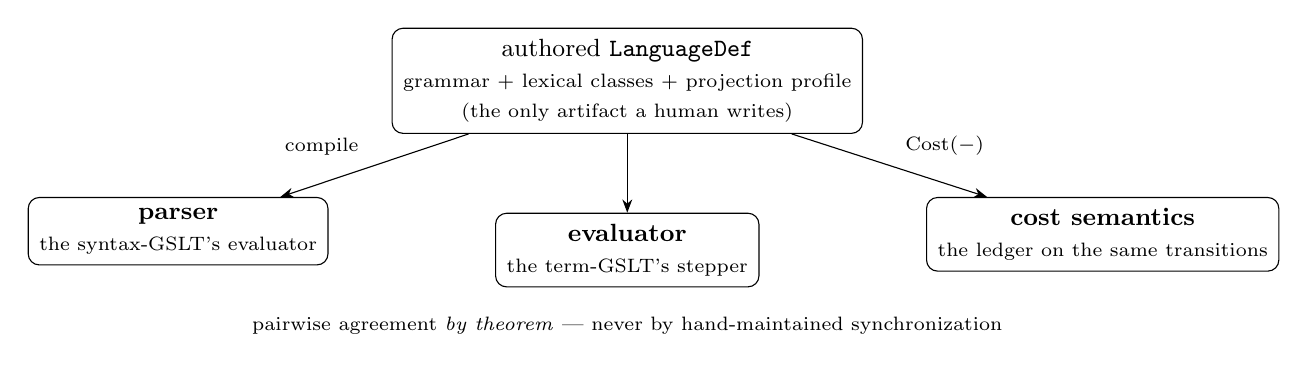
\begin{tikzpicture}[
  box/.style={draw, rounded corners, align=center, inner sep=4pt,
    font=\small}]
\node[box] (root) {authored \code{LanguageDef}\\
  {\scriptsize grammar $+$ lexical classes $+$ projection profile}\\
  {\scriptsize (the only artifact a human writes)}};
\node[box, below left=8mm and 8mm of root] (parser)
  {\textbf{parser}\\{\scriptsize the syntax-GSLT's evaluator}};
\node[box, below=10mm of root] (eval)
  {\textbf{evaluator}\\{\scriptsize the term-GSLT's stepper}};
\node[box, below right=8mm and 8mm of root] (cost)
  {\textbf{cost semantics}\\{\scriptsize the ledger on the same
    transitions}};
\draw[-{Stealth}] (root) -- (parser)
  node[midway, above left, font=\scriptsize]{compile\;};
\draw[-{Stealth}] (root) -- (eval);
\draw[-{Stealth}] (root) -- (cost)
  node[midway, above right, font=\scriptsize]{\;$\mathrm{Cost}(-)$};
\node[below=2.5mm of eval, font=\scriptsize, align=center]
  {pairwise agreement \emph{by theorem} --- never by hand-maintained
   synchronization};
\end{tikzpicture}
\end{center}

\noindent
The compositional discipline is enforced starvation: no derived component
has any information channel back to the language except the proved
interfaces, so there is nothing left \emph{to} drift.  The formal side lives in the
Mettapedia Lean development and is sorry- and axiom-clean across the
roughly fifteen-thousand-line module family; the axiom reports below were
re-checked against the kernel at the time of writing.  The pipeline, for
the Metamath instance:

\begin{center}
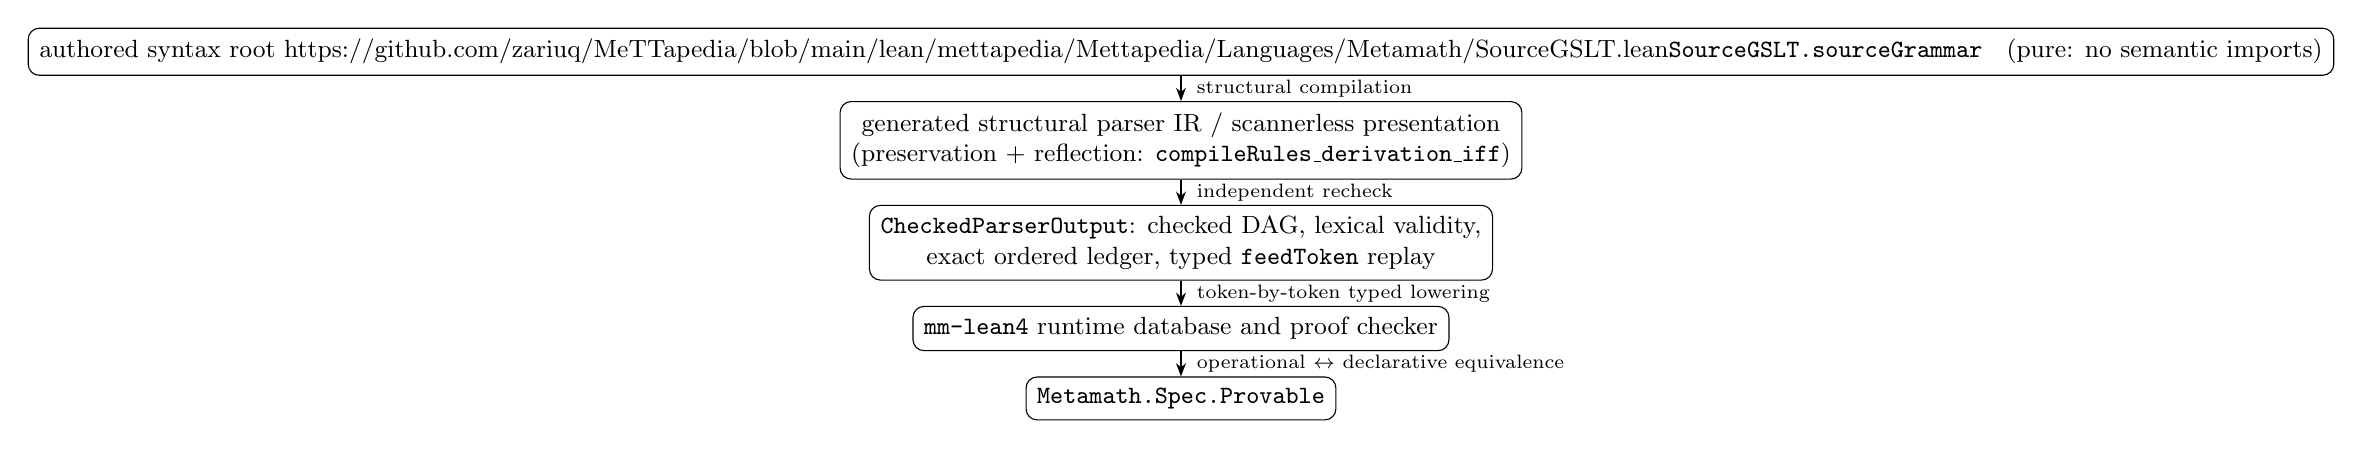
\begin{tikzpicture}[node distance=3.2mm,
  box/.style={draw, rounded corners, align=center, inner sep=4pt,
    font=\small}]
\node[box] (root) {authored syntax root
  \href{https://github.com/zariuq/MeTTapedia/blob/main/lean/mettapedia/Mettapedia/Languages/Metamath/SourceGSLT.lean}{\code{SourceGSLT.sourceGrammar}}
  \; (pure: no semantic imports)};
\node[box, below=of root] (ir) {generated structural parser IR / scannerless
  presentation\\ (preservation $+$ reflection:
  \code{compileRules\_derivation\_iff})};
\node[box, below=of ir] (cert) {\code{CheckedParserOutput}: checked DAG,
  lexical validity,\\ exact ordered ledger, typed \code{feedToken} replay};
\node[box, below=of cert] (mm) {\code{mm-lean4} runtime database and proof
  checker};
\node[box, below=of mm] (spec) {\code{Metamath.Spec.Provable}};
\draw[-{Stealth}] (root) -- (ir)
  node[midway,right,font=\scriptsize]{\;structural compilation};
\draw[-{Stealth}] (ir) -- (cert)
  node[midway,right,font=\scriptsize]{\;independent recheck};
\draw[-{Stealth}] (cert) -- (mm)
  node[midway,right,font=\scriptsize]{\;token-by-token typed lowering};
\draw[-{Stealth}] (mm) -- (spec)
  node[midway,right,font=\scriptsize]{\;operational $\leftrightarrow$
    declarative equivalence};
\end{tikzpicture}
\end{center}

\noindent
Parsing and checking remain separate judgments at every stage; the
composition modules join them by theorem.  Generically, the same chain
reads as a sequence of seams, each crossed only inside a certificate:

\begin{center}
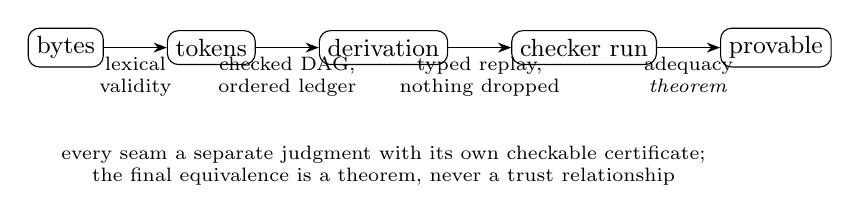
\begin{tikzpicture}[node distance=8mm,
  st/.style={draw, rounded corners, inner sep=3pt, font=\small}]
\node[st] (b) {bytes};
\node[st, right=of b] (t) {tokens};
\node[st, right=of t] (d) {derivation};
\node[st, right=of d] (c) {checker run};
\node[st, right=of c] (p) {provable};
\draw[-{Stealth}] (b) -- (t)
  node[midway, below, font=\scriptsize, align=center]{lexical\\ validity};
\draw[-{Stealth}] (t) -- (d)
  node[midway, below, font=\scriptsize, align=center]{checked DAG,\\
    ordered ledger};
\draw[-{Stealth}] (d) -- (c)
  node[midway, below, font=\scriptsize, align=center]{typed replay,\\
    nothing dropped};
\draw[-{Stealth}] (c) -- (p)
  node[midway, below, font=\scriptsize, align=center]{adequacy\\
    \emph{theorem}};
\node[below=9mm of d, font=\scriptsize, align=center]
  {every seam a separate judgment with its own checkable certificate;\\
   the final equivalence is a theorem, never a trust relationship};
\end{tikzpicture}
\end{center}

\paragraph{The generic compiler and its two-sided correspondence.}  A
generic, language-agnostic compiler turns the grammar fragment of any
\code{LanguageDef} into structural parser rules.  Three theorems bound its
authority.  Changing any non-syntax field of the declaration cannot change
the generated rules (\code{compileRules\_eq\_of\_terms\_eq}); generated-rule
actions retain the independently decoded terminal/child skeleton, so a rule
cannot silently drop, duplicate, or reorder children
(\code{compileRules\_action\_shape}); and --- the load-bearing result ---
derivability in the generated structural intermediate form is
\emph{equivalent} to derivability in the authored grammar at the
ordered-token boundary (\code{compileRules\_derivation\_iff}: preservation
\emph{and} reflection, a genuine second relation rather than equality by
definition; kernel axioms exactly \code{propext},
\code{Classical.choice}, \code{Quot.sound};
\href{https://github.com/zariuq/MeTTapedia/blob/main/lean/mettapedia/Mettapedia/GSLT/Parsing/LanguageDefSyntaxCorrespondence.lean}{\code{GSLT/Parsing/LanguageDefSyntaxCorrespondence.lean}}).

\paragraph{Checked languages: two laws, crowns for free.}  The reusable
\code{CheckedLanguage} interface packages what any language must supply to
close the loop from bytes to meaning: a syntax-only root, a lexical
relation, a lowering into a checker, and a declarative judgment, subject to
exactly two laws --- exact lowering and checker adequacy.  From those two
laws the certificate-indexed and whole-pipeline crown theorems
(\code{pipelineAccepts\_iff\_parserAccepts\_and\_declarative} and kin) are
derived \emph{once, generically}; the generic composition layer
(\href{https://github.com/zariuq/MeTTapedia/blob/main/lean/mettapedia/Mettapedia/GSLT/CheckedLanguage.lean}{\code{GSLT/CheckedLanguage.lean}})
proves them with \emph{no axioms at all}.  Parsing and checking remain
separate judgments throughout: the composition joins them by theorem, and
neither the parser nor its certificate is ever allowed to authorize a
theorem.

\begin{center}
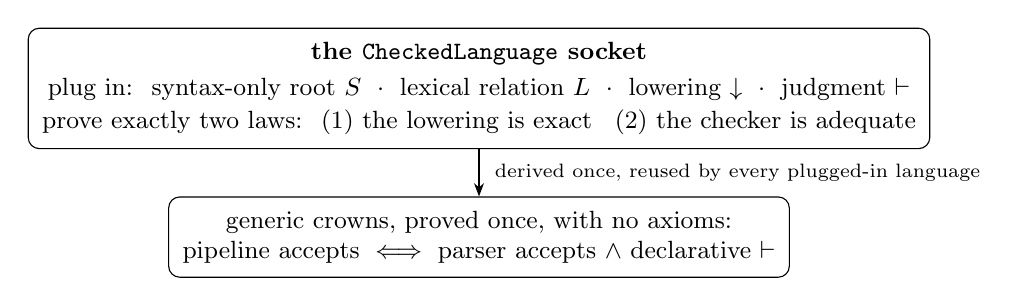
\begin{tikzpicture}[
  box/.style={draw, rounded corners, align=center, inner sep=5pt,
    font=\small}]
\node[box] (socket) {\textbf{the \code{CheckedLanguage} socket}\\[2pt]
  plug in:\; syntax-only root $S$ \;$\cdot$\; lexical relation $L$
  \;$\cdot$\; lowering $\downarrow$ \;$\cdot$\; judgment $\vdash$\\[1pt]
  prove exactly two laws:\; (1) the lowering is exact
  \;\;(2) the checker is adequate};
\node[box, below=6mm of socket] (crown)
  {generic crowns, proved once, with no axioms:\\
   pipeline accepts $\iff$ parser accepts $\wedge$ declarative $\vdash$};
\draw[-{Stealth}] (socket) -- (crown)
  node[midway, right, font=\scriptsize]
  {\;derived once, reused by every plugged-in language};
\end{tikzpicture}
\end{center}

\noindent
The expensive theorem is proved once, about the socket; each further
language pays only its own two laws.  That, rather than any property of
Metamath itself, is why the Metamath instance below is a template.

\paragraph{The Metamath vertical slice: a parser-to-provability crown.}
The first full instance runs from raw Metamath bytes to formal
provability.  The authored Metamath syntax root is a \emph{pure} grammar
--- a semantic firewall: it imports only the generic grammar-inference
layer, and the generic compiler contains no Metamath-specific names.  On
top of it, \code{CheckedParserOutput} demands an independently checked
grammar DAG, lexical validity, exact ordered-token agreement, and a
successfully constructed verified reader; \code{TypedLoweringCertificate}
pairs every classified source token, in order and without insertion or
omission, with an actual \code{ParserState.feedToken} transition of the
verified \code{mm-lean4} checker, and proves that the instrumented
execution erases to the production checker database.  The crown
(\code{generatedParserAndCheckerAcceptance\_iff\_specProvability}) then
states that generated-parser-plus-checker acceptance is equivalent to
declarative acceptance by \code{Metamath.Spec.Provable} --- kernel axioms
again exactly \code{propext}, \code{Classical.choice}, \code{Quot.sound}.
The reverse direction cannot manufacture syntax evidence: it is indexed by
an existing checked parser output whose certificates have already passed
their independent checkers.  The crown, verbatim from
\href{https://github.com/zariuq/MeTTapedia/blob/main/lean/mettapedia/Mettapedia/Languages/Metamath/SourceGSLTCheckerAlignment.lean}{\code{SourceGSLTCheckerAlignment.lean}}:

\begin{lstlisting}
def GeneratedParserAndCheckerAccepts
    {bytes : ByteArray} (output : CheckedParserOutput bytes)
    (label : String) (formula : Metamath.Verify.Formula) : Prop :=
  TypedLoweringCertificate bytes output.source /\
    ImplementationAccepts bytes label formula

theorem generatedParserAndCheckerAcceptance_iff_specProvability
    {bytes : ByteArray} (output : CheckedParserOutput bytes)
    (label : String) (formula : Metamath.Verify.Formula) :
    GeneratedParserAndCheckerAccepts output label formula <->
      DeclarativeAccepts bytes formula
\end{lstlisting}

\noindent
Executable closure evidence: seven checked
ordered ledgers (demo0, MIU, Peano, disjoint-variable and proof-format
cases, and an authentic propositional \code{set.mm} slice) in exact
object-level agreement with independent \code{mm-lean4} output;
normal/compressed proof agreement; five malformed-source rejections;
killed mutations across labels, disjoint-variable conditions, compressed
proofs, declaration order, AST, lexer, and semantic references; and
byte-identical regeneration of both generated Metamath artifacts from the
Lean root.

\paragraph{From parser-GSLT to checker-GSLT: source-owned inference.}
Since the vertical slice above was sealed, the same authored root has
grown a second semantic derivation: Metamath \emph{checking} itself as a
source-owned GSLT.
\href{https://github.com/zariuq/MeTTapedia/blob/main/lean/mettapedia/Mettapedia/Languages/Metamath/SourceGSLTOperations.lean}{\code{SourceGSLTOperations.lean}}
is the single authored bridge from the source grammar to the streaming
fold and indexed-checker operations: node contracts are \emph{computed}
from the parameter sorts of the source productions, and lexical references
resolve through the same literal tables that generate the parser.
\href{https://github.com/zariuq/MeTTapedia/blob/main/lean/mettapedia/Mettapedia/Languages/Metamath/SourceGSLTState.lean}{\code{SourceGSLTState.lean}}
gives those operations their scoped-state semantics (frames, scope
closing, global object identities) with no reference to the
\code{mm-lean4} runtime database, and
\href{https://github.com/zariuq/MeTTapedia/blob/main/lean/mettapedia/Mettapedia/Languages/Metamath/SourceGSLTNormalTheorem.lean}{\code{SourceGSLTNormalTheorem.lean}}
admits a normal-theorem transition only through an exact source-owned
proof-occurrence tree over the pre-insertion database prefix ---
independent of the \code{mm-lean4} execution function.  Operational and
declarative adequacy
(\code{SourceInferenceOperationalAdequacy},
\href{https://github.com/zariuq/MeTTapedia/blob/main/lean/mettapedia/Mettapedia/Languages/Metamath/SourceInferenceDeclarativeAdequacy.lean}{\code{SourceInferenceDeclarativeAdequacy.lean}})
connect this source-derived checker semantics to Metamath's declarative
semantics with every database, frame, declaration, and disjointness
premise derived from the same validated source prefix; the crown
(\code{NormalTheoremStep.toSemanticProvable}) was re-verified for this
section at kernel axioms exactly \code{propext}, \code{Classical.choice},
\code{Quot.sound}, with the module family sorry-free.  Export modules
(\code{SourceGSLTParserExport}, \code{SourceGSLTOperationsMeTTaExport})
regenerate both engine-facing artifacts from the root, and a native
inference-staging consumer (\code{lib\_parse\_inference\_native}, with its
benchmark harness) carries the operations export into the engine.  The
Metamath instance is thereby the template the programme intends to
replicate: \emph{one} authored root from which the parser, the checker
operations, and their adequacy theorems are all derived, ready to be
instantiated across a curriculum of further language definitions.

\paragraph{Declaration-level co-evolution with the shipped checker
(August 2026).}  The source-owned semantics above has since been joined to
the verified implementation at the level of individual transitions.  Every
accepted source declaration step --- \code{\$c}, \code{\$v}, \code{\$d},
\code{\$f}, \code{\$e}, assertion insertion for \code{\$a}/\code{\$p}, and
scope push/pop/completion --- is now matched by the \emph{shipped}
\code{mm-lean4} database operation it corresponds to (the per-token
declaration inserts, the checked hypothesis insertion, the axiom insertion
including its mandatory-frame trim), and the whole statement fold co-evolves
with the implementation database from the initial states with no supplied
premises (\code{default\_initial\_applyPayloads} in
\code{SourceGSLTRuntimeCoEvolution.lean}).  Two identifications carry the
weight: the implementation's mutable mandatory-frame computation is proved
equal to the specification's mandatory frame
(\code{trimFrame'\_eq\_mandatory}), and the accepted pipeline's own
classified stream supplies its lexical evidence
(\code{runSource\_selfLexicalized\_derives}), so neither the frame nor the
token boundary is ever assumed.  A deliberate honesty distinction
structures the remaining work: results proved from one accepted source run
and one checked byte presentation are kept as \emph{parallel} certificates
until the classified stream is bound to the exact bytes the verified reader
consumed, each \code{\$p} obligation's normal or compressed proof is
discharged from the reader's own chronology (with verified and
incomplete-\code{?} outcomes as disjoint results), and the source fold is
related to the production reader by a prefix-wise simulation in which
reader microsteps are administrative and completed statements are the
observable steps.  The normal-proof discharge has been constructed against
the production reader trace; the compressed analogue and the whole-prefix
simulation are in active development.

\paragraph{Second consumers and the engine loop.}  Megalodon has an honest
second-consumer skeleton that reuses the generic signatures and crown ---
deliberately \emph{not} yet claimed as an instance, since its verified
checker and adequacy laws remain to be built.  On the engine side, the
generated Metamath grammar artifact is consumed directly by \CeTTa{}
(\code{lib\_parse\_metamath\_grammar\_generated\_v0.metta}) alongside the
\code{lib\_parse} family and the signature-driven ABT binder layer in the
Prime integration lane; the full engine-side parse gate (Metamath, ABT,
and native-reader tests) was re-run green for this section.  Honest
boundaries: the tested \code{set.mm} artifact is a nontrivial authentic
slice, not the full corpus; raw byte-to-token completeness is secured per
accepted certificate by exact typed reader replay, with a universal
raw-byte characterization theorem remaining future work; and the
declaration-level co-evolution above becomes a single bidirectional
statement only once the same-presentation binding, per-\code{\$p}
discharge, and prefix simulation land, as itemized in the preceding
paragraph.

\subsection{MeTTa Zero: a two-operation kernel with native proof evidence}
\label{sec:zero-oslf-nik}

MeTTa Zero is the compact executable specimen for extending the preceding
programme from parsing to language semantics and compilation.  Assuming
s-expressions with variables, an occurrence bag $S$, matching with
substitution, and a declared grounding capability, its kernel has only two
public semantic operations.  Write $v$ for a fresh wildcard and abbreviate
the interpreted result bag by $R_S(x)$:

\begin{align}
\mathsf{query}_S(p,t)
  &= \biguplus_{a\in S}
       \{\,t\theta \mid \theta\in\mathsf{match}(p,a)\,\},
       \label{eq:zero-query}\\
R_S(x)
  &= \left(\biguplus_{(=\,l\,r)\in\mathsf{query}_S(v,v)}
       \{\,r\theta \mid \theta\in\mathsf{match}(l,x)\,\}\right)
       \uplus \mathsf{ground}(x),
       \label{eq:zero-results}\\
\mathsf{eval}_S(x)
  &= \begin{cases}
       R_S(x), & R_S(x)\neq\varnothing,\\
       \{x\},  & R_S(x)=\varnothing.
     \end{cases}
     \label{eq:zero-eval}
\end{align}

Equations are therefore ordinary queryable atoms, not entries in a private
rule store; evaluation obtains them through the same public query as user
programs.  Grounding is a declared library capability, and a capability's
decline leaves an uninterpreted subject inert rather than turning ignorance
into an empty result.  The coproducts are occurrence coproducts: duplicate
facts, rules, matches, and answers remain distinct.  A recursive semantic
runner, continuations, pending work, and \code{reify} compose over this
kernel; they are not silently folded into Equations~\ref{eq:zero-query}--
\ref{eq:zero-eval}.  The current runner is consequently retained as a
versioned experimental profile while its abstract laws and cross-dialect
interpretations are established.

\paragraph{One semantic root, three derived uses of native types.}
The Lean development sends Zero's actual composed
\code{ExtendedLanguageDef} and relation environment through OSLF, rather
than constructing a parallel transition relation:

\begin{center}
$\text{Zero language definition}
  \longrightarrow \text{relation-backed OSLF span}
  \longrightarrow \text{native types and certificates}$
\end{center}

\noindent
The resulting information has three distinct, proved uses.

\begin{enumerate}
\item \textbf{Spatial classification.}  Generated headed types recognize
  equation atoms and the exact query/evaluation request and answer
  constructors.  The constructor list is computed from the language term
  grammar (\code{zero\_constructorTypes}), rather than maintained as a
  second inventory.
\item \textbf{Behavioral evidence.}  Exact query and evaluation diamond
  theorems identify the OSLF diamond with existence of an answer in the
  corresponding Zero occurrence bag.
  Proof-relevant finite certificates are sound and complete for this
  admitted fragment.  Generic predecessor-universal \code{box} evidence
  deliberately fails closed until finite predecessor enumeration, an
  invariant, or coinductive evidence is supplied.
\item \textbf{Compilation analysis.}  Constructor/arity head signatures
  select the query or evaluation production without inspecting every rule.
  Unsupported forms take the complete rule-table fallback.  The selected
  plan is proved equal both to the generic executor and to the authored
  Zero interpreter under the exact occurrence-bag observer
  (\code{executeAuthoredNativePlanned\_eq},
  \code{nativePlanned\_eq\_authored}).  Thus the analysis establishes a
  safe shape for generated native dispatch; exporting that index into the
  C plan ABI is an implementation step, not a new semantic decision.
\end{enumerate}

The distinction between the second and third uses is load-bearing.  A
diamond records that at least one suitable transition exists; it does not
record how many occurrences produced it.  The negative theorem
\code{diamond\_equal\_but\_edge\_counts\_differ} exhibits two spans with
the same diamond observation and different edge multiplicities.  Native
types may therefore guide dispatch and justify existence claims, but they
cannot replace Zero's bag observer.

The generic native-type construction is in
\href{https://github.com/zariuq/MeTTapedia/blob/main/lean/mettapedia/Mettapedia/OSLF/Framework/NativeTypeTheory.lean}{\code{OSLF/Framework/NativeTypeTheory.lean}};
the concrete Zero theorems are in
\href{https://github.com/zariuq/MeTTapedia/blob/main/lean/mettapedia/Mettapedia/Languages/MeTTa/MeTTaZeroLanguageAdequacy.lean}{\code{MeTTaZeroLanguageAdequacy.lean}}.

\paragraph{From a trace to an independently replayed proof.}
ProofGSLT's open derivations now carry an ordered context of explicit
premises, with a generic semantic-induction theorem: if every local rule
application preserves meaning and every open premise has its declared
meaning, the derived conclusion has its meaning.  Zero instantiates this
interface with one admitted eight-rule presentation: six spatial rules and
two behavioral liveness rules.  A liveness rule cannot mint an answer edge
by itself; it requires a query-row or evaluation-row premise tied to an
actual occurrence in the interpreted Zero relation.

The bridge in
\href{https://github.com/zariuq/MeTTapedia/blob/main/lean/mettapedia/Mettapedia/OSLF/Framework/NativeTypeProofGSLT.lean}{\code{OSLF/Framework/NativeTypeProofGSLT.lean}}
turns an accepted open \code{WireArticle} into MIK semantic authority and
exposes the corresponding checked-lowering obligation for a native NIK.
All eight Zero rule schemas have local semantic-preservation proofs.  A
positive article plus its true row premise entails the OSLF behavioral
claim; the negative canary changes the article to an out-of-range premise
reference and is rejected.  This is proof-producing compilation structure,
not merely a diagnostic trace.

\paragraph{The current C boundary.}
The executable Zero compiler separately emits a deterministic, hash-linked
build certificate for

\begin{center}
$\text{authored sources}\longrightarrow
  \text{admitted rules}\longrightarrow
  \text{CGP1 plan}\longrightarrow
  \text{generated C/H bytes}$.
\end{center}

\noindent
An independent build-time C checker rereads the sources, replays admission,
compares every compiled rule structurally, and checks the exact generated
artifacts; tampering and nondeterministic regeneration are gated.  This
checker is not linked into the ordinary \CeTTa{} executable, so normal
execution pays no certificate-parsing or trace-retention cost.  The claim is
nevertheless bounded: the certificate proves structural chain of custody,
not yet that executing CGP1 or the generated C realizes all authored Zero
observations.  The open row premises above are not yet closed by
authenticated C execution receipts, and the C checker is not yet generated
from the single ProofGSLT acceptance predicate.  These are the remaining
seams between the working build attestation and end-to-end NIK replay.  The
C checker is independent of the Python producer, but deliberately reuses the
generic C parser, admission path, and plan decoder; the resulting common-mode
boundary is another reason the ProofGSLT replay correspondence remains
necessary.

\section{MeTTa Prime: A Lazy Sibling Language}
\label{sec:prime}

\code{--lang prime} is a \emph{distinct} MeTTa language sharing \CeTTa{}'s
implementation substrate: branch-local call-by-need with call-time choice
as the ordinary application semantics.  It is not an extension of \HE{}
and does not reduce to \HE{} under erasure; the ``\HE{} unchanged'' gates
that accompany every Prime tranche establish noninterference on shared
code, not a semantic relationship.  Appendix~\ref{app:prime-spec} distills
the living specification; the highlights are:

\begin{itemize}
\item \textbf{Need cells.}  Suspensions are opaque runtime capabilities
  with an immutable origin and a checked cache state machine; completed
  values and stable faults memoize, blackholes and interruptions remain
  retryable.  Call-time choice makes sharing observable: one delayed
  choice used twice yields only correlated outcomes.
\item \textbf{Equation dispatch.}  Rewrite candidates for one call share
  one source suspension per argument; the candidate \emph{frontier} is a
  scheduling notion, never a kind of equality.  The static frontier
  policies were all refuted as complete semantics by a common law audit;
  the selected direction keys producer identity to the Need cell itself
  (application and source positions are subscription edges), with a
  policy-neutral certified control layer under which breadth-first,
  depth-first, ranked, and permuted exploration provably preserve the
  answer bag.
\item \textbf{Faults as data.}  Ordinary evaluation propagates faults;
  explicit structural observers inspect a fault atom as data, so
  error-conditional programming is a deliberate boundary rather than an
  accident of evaluation order.
\item \textbf{Exact outcome carrier.}  Prime's computational zero is the
  absence of occurrences; the symbol \code{Empty} is ordinary inert data,
  and the empty expression \code{()} remains a unit datum rather than choice
  zero.  The internal \code{EvalOutcome} carries the ordered occurrence bag
  (ordinary values and fault occurrences together), completion reason, and
  budget state before any compatibility projection.  Its derived zero
  observation distinguishes complete zero, nonzero, and pending zero, so an
  incomplete frontier cannot be laundered into a proof of absence.
\item \textbf{Anonymous variables.}  Bare \code{\$} is a fresh anonymous
  variable per occurrence (it matches any term and binds nothing
  referenceable); named variables retain co-reference.  This is
  Prime-only: \HE{} bare \code{\$} remains governed by the \HE{} written
  contract.
\item \textbf{Dependence-aware evidence export.}  A shared-cause
  discriminator is reproduced natively: two syntactically distinct
  explanations sharing one producer outcome yield exact possible-world
  probability $1/2$ where naive independent-explanation disjunction gives
  $3/4$.  Prime exports dependence structure to evidence consumers;
  probability and proof authority never move inside the evaluator.
\end{itemize}

Early experiments host proof search as type inhabitation over the lazy
frontier (Metamath-style problems with premise selection and
reduction-ordering guidance), which is the intended cognitive-language
role: demand-driven search over an inspectable frontier, with
claim-bearing results lowered to an external checker rather than asserted
by execution.

\paragraph{Practicality.}
Ground-call memoization --- an off-by-default table admitting only
ground, canonical, completed, effect-pure calls at an exact space
revision, replayed as whole bags --- makes na\"ive recursive workloads
practical (na\"ive \code{fib} runs in fractions of a second).  Judgment
evaluation records its evidence at constant cost per step, so budgeted
judgments scale linearly with the run they observe.  Prime's
per-occurrence bookkeeping lives behind a single lazy extension pointer
that is \code{NULL} on the \HE{} lane, so the shared evaluator carries
no Prime overhead: paired storage ladders place the Prime-bearing
engine below a Prime-free build on peak memory.
Appendix~\ref{app:algorithms} records the algorithms and the
asymptotic analysis.

\section{Related Work}

\paragraph{Concurrent constraint programming.}
Saraswat et al.~\cite{saraswat1988} established the theoretical
framework for detecting stable properties of networks in concurrent
logic programming languages.  Their cc($\downarrow$,$|$) language,
with Tell/Ask on shared variables over a monotonic constraint store,
provides the semantic model that most closely matches \HE{}/\CeTTa{}'s
\code{match~\&self} evaluation.  The distinction between monotonic
constraint stores and independent-scope evaluation (Flat Concurrent
Prolog) precisely characterizes the semantic boundary between \HE{} and
\PeTTa{}.

\paragraph{MeTTa ecosystem.}
The MeTTaIL boot compilation pipeline~\cite{mettail} provides a
contract-first, Lean-backed compilation path for MeTTa stdlib modules,
complementing \CeTTa{}'s direct evaluation approach.  The Mettapedia
formalization project provides the Lean specifications (\code{EvalSpec},
\code{MeTTaEval}, \code{MatchSpec}) that ground both the translation
proof and the \CeTTa{} evaluator design.  The PLN (Probabilistic Logic
Networks) framework uses MeTTa's backward chaining extensively; the
typed chainer pattern from Nil Geisweiller's \code{nilbc.metta} is
the standard PLN idiom that works across all three runtimes.

%% ────────────────────────────────────────────────────────────────────
\section{Conclusion}

\CeTTa{} demonstrates that a direct C implementation of the MeTTa
evaluator is competitive with \PeTTa{} on inference workloads, but not
uniformly faster.  In the fresh reruns reported here, \CeTTa{} wins on
startup-dominated shallow inference and on several genomic-inference
rows (the 183-pair PLN evidence core and the 1{,}411{,}430-hypothesis
deep genomic backward-chaining row), while \PeTTa{} wins decisively on
pure branching search (the 85{,}013-proof Metamath row).  A
cross-engine chaining suite (Section~\ref{sec:chaining-suite})
confirms that \CeTTa{}'s shallow advantage is a startup-and-dispatch
effect rather than a scaling property.  Historical rows whose current
drivers are unresolved or no longer the same computation as their old
headline---the old miner speed table and BTree---are
excluded from the revised
benchmark ladder rather than carried forward on trust.  Throughout,
\CeTTa{} maintains
oracle-verified correctness across a 535-test MeTTa regression suite and a
23-case \HE{} I/O semantic conformance gate against upstream
\HE{}~v0.2.10.
The sorry-free Lean proof of \HE{}$\leftrightarrow$\PeTTa{} semantic
correspondence (5{,}400+ lines, 0~sorries), including import
commutativity and operational bridges for state and space allocation,
establishes that MeTTa's three runtimes are semantically compatible
on the shared fragment.  The compiled \code{.act} space format via
MORK enables zero-copy indexed loading, demonstrated at the 100k-atom
scale, with the large-scale attach path still under repair.
On the process-calculus side, the \RhoCalc{} reaction machine's
eval-at-\textsc{comm} semantics now has a witness-free, axiom-clean Lean
characterization (Section~\ref{sec:rho-lean}): the quiescent run of the
canonical payload-evaluation process is exactly its structurally observable
outcome set, with no certification witness in the carrier.

Beyond raw performance, \CeTTa{} now treats its own semantics as a
first-class object.  The profile family makes \code{he-compat} (literal
Rust \HE{}) and the principled \code{he} line distinct, recorded
semantic products; the reflective modal layer exposes the one-step
reduction relation---$\Diamond$, $\Box$, normal-form---to MeTTa
programs themselves, aligned with the Lean OSLF derivation; and the
small-step rule table makes the first reduction-rule classes named,
reflectable, and removable, with rule-removal tests proving the engine
depends on the declared rules rather than on duplicate hidden branches.
The congruence bug that motivated this weld---an argument-congruence
rule silently missing from the one-step relation on three branches at
once---is exactly the drift class this architecture eliminates.
MeTTa Zero makes the staged version of the same discipline concrete
(Section~\ref{sec:zero-oslf-nik}): its public query and query-derived
evaluator generate one relation-backed OSLF span; native types provide
checked behavioral evidence and safe constructor-indexed planning; and
open ProofGSLT articles cross into MIK authority and NIK replay without
discarding their semantic row obligations.  The negative multiplicity
theorem prevents that modal analysis from being mistaken for the exact-bag
semantics it accelerates.

The 1.4 development line also turns much of the earlier machine roadmap into
runtime structure: revision-pinned \code{MatchDecision} and bounded
\code{RuleMachine} artifacts, an explicit \PeTTa{} heap machine, exact Prime
outcomes, and observer-safe substitution fusion.  Its counted \PathMap{}
backend is now a real generic query route rather than a bootstrap-only store.
The answer-first August audit found and removed both an effectively complete
candidate scan and a quadratic mutation/index-rebuild loop; at 7{,}381
HexLife cells Prime improves from 2.89\,s native to 2.53\,s on \PathMap{},
while \PeTTa{} remains near backend parity (22.21 versus 22.71\,s).  The
dialect-honest SWI table shows no broad performance collapse, but preserves
two important open targets: \PeTTa{} control/allocation overhead on reverse
and Roman, and high-cardinality \PeTTa{} control even after storage lookup is
no longer the bottleneck.

Tilepuzzle is settled capacity evidence again, but not a \CeTTa{} speed
win.  The normalized contract counts 181{,}440 reachable boards
including the start state; the \PeTTa{} native example's 181{,}441
self-check is a counter-convention difference, not an extra board.  The
\PeTTa{} native rerun remains much faster (1.40\,s, 121\,MiB), while the
\CeTTa{} result is the repaired capacity row: the full board-count search
now completes in 8.80\,s at 233\,MiB after the tail-safe
evaluation-arena garbage collector (Section~\ref{sec:tilepuzzle-gc}).
Trail-style rollback, bindings builders, and arena mark/reset remain
candidates for further improving search-heavy workloads without
converting \CeTTa{} into a Prolog engine.
The guiding principle: \emph{backtracking should be rare, local, and
hidden---not global, ambient, or user-visible.}

\paragraph{Future work.}
\begin{itemize}
\item \textbf{Complete HE one-step coverage:} equation matching is
  table-routed; migrate the special forms (\code{chain}, \code{let},
  \code{let*}, \code{case}, \code{switch}) one rule class at a time,
  each with bag-equality and rule-removal gates.
\item \textbf{\code{--compile-langdef} codegen:} a generator emitting
  both the reflectable pack and specialized C for the hot evaluator
  under one shared source digest, extending the
  \code{--compile-stdlib} blob precedent; export Zero's proved native
  head/dependency index into that plan ABI, retain the complete-table
  fallback, and keep an evaluate-by-iterating-one-step mode as reference
  oracle.
\item \textbf{Zero NIK closure:} generate the native checker from the one
  ProofGSLT acceptance predicate; define authenticated query-row and
  capability-receipt codecs that discharge open articles; prove native
  codec/replay correspondence; then compose the compilation certificate
  with a separate execution receipt.  Proof machinery remains a build-time
  or on-demand path, absent from the ordinary runtime hot path.
\item \textbf{Small-step / official-HE correspondence:} the
  \code{HESmallStep} relation and its OSLF span exist in Lean
  (proven; zero sorries); the remaining climb is the delimited
  collapse/simulation theorems connecting it to the fine
  \code{mettaHE} instruction machine.
\item \textbf{Bounded modal operators:} fuel-bounded
  \code{reachable-within} ($\Diamond^{\le k}$) and
  \code{invariant-within} ($\Box^{\le k}$) over the now-faithful
  one-step relation.
\item \textbf{Complete the local search-machine transition:} the explicit
  \PeTTa{} heap, choice, continuation, and rollback core is working.  Next
  move mode/relation clause discrimination into the outer loop, compact
  activation environments and shared continuations, and remove Prime's
  retained per-result Need/receipt state on large materialized bags.  Keep
  tilepuzzle and the same-source SWI portfolio as answer-first gates.
\item \textbf{Versioned heterogeneous realization:} implement the open
  $\mathsf{snapshot}\times\mathsf{operator\ plan}\to
  \mathsf{delta}\times\mathsf{receipt}$ boundary with exact occurrence
  evidence, stale-receipt rejection, backend-specific parallel admission,
  and mandatory serialization fallback.  OS-thread lowering follows
  semantic commutation \emph{and} backend resource compatibility; neither
  native nor \PathMap{} physics becomes language semantics.
\item \textbf{Indexed shared-space engine:} replace the synchronized native
  candidate view, where admitted, with direct \PathMap{} descent and product
  cursors; add leapfrog triejoin, grouped aggregation, and persistent
  snapshot/fork experiments.  Preserve the SpaceEngine boundary (formalized in
  \code{SpaceEngineBoundary.lean}: native $\subset$ pathmap $\subset$ mork,
  with ACT as artifact-only boundary; \code{ACTArtifactBoundary.lean}
  classifies \code{open-act}/\code{load-act!}/\code{dump!} as storage seams).
  Retain authoritative native fallback wherever a direct route cannot preserve
  the named observer.
\item \textbf{MM2 as MeTTa data (working):} MM2 exec rules are atoms in
  MORK-backed spaces.  MeTTa creates, inspects, rewrites, and steps them
  through the ordinary space API\@.  \code{step!} is the execution interface;
  \code{.mm2} files import via \code{include}/\code{import!}.  MeTTa can
  pattern-match over MM2 code to analyze or transform programs---the
  meta-language relationship is native.  The separate fail-closed hosted
  translator is useful but incomplete: add runtime priority-queue semantics
  with explicit \code{exec} consumption, replace quadratic distinct-count
  grouping with one grouped pass/backend operator, and extend source/sink
  coverage only under exact differential witnesses.
\item \textbf{\PathMap{} algebra (working):}  \CeTTa{} already exposes MORK's
  \PathMap{} substrate through the \code{mork:} builtins: the lattice
  operations \code{mork:join}, \code{mork:meet}, \code{mork:subtract}, and
  \code{mork:prefix-restrict}; read-only zipper navigation; product-zipper
  Cartesian joins over two to four spaces; and overlay-zipper cursors.
  Underneath, the Rust substrate is substantial---zipper navigation
  (5{,}800 lines), product-zipper joins (2{,}000 lines), and the lattice
  operations (1{,}600 lines)---and a Lean formalization (46 files, 19K+ lines)
  proves the three-phase execution protocol, fold-level aggregation, and
  \PathMap{} lattice correspondence.  What remains future is surfacing MORK's
  aggregating sink types (count, sum, head, hash, and, Z3, WASM) and source
  types (BTM, ACT, equality/inequality constraints) at the MeTTa level: the
  kernel implements them, but the \code{mork:} API does not yet expose them.
\item \textbf{HO search engine:} Lash-inspired SAT-driven proof
  search for PLN and type-directed synthesis.  PicoSAT as
  embedded SAT solver.  Separate from the evaluator.
\item \textbf{Translator CLI:} \code{translate.sh} with
  \code{he2petta}/\code{petta2he}, recursive and bundle modes.
  Lean proof covers pure fragment + state + spaces (0~sorries).
\item \textbf{Reaction-semantics formalization:} extend the witness-free
  eval-at-\textsc{comm} characterization (Section~\ref{sec:rho-lean}) from the
  single-reaction bag fragment to concurrent and persistent reactions, and
  relax the hash-set-free channel side condition.
\item Full pattern miner on \CeTTa{} end-to-end
  ($\sim$12$\times$ speedup over \PeTTa{}).
\end{itemize}

\appendix

\section{\LeaTTa{} Cross-Check Appendix}
\label{app:leatta}

\LeaTTa{} is a Lean~4 MeTTa runtime and proof development that is useful
as an independent semantic cross-check for the \HE{}-facing core of
\CeTTa{}.  The local checkout used for the measurements in this
appendix was a clean \LeaTTa{}~1.0.6 tree at
\href{https://github.com/MesTTo/LeaTTa}{\code{github.com/MesTTo/LeaTTa}},
commit
\href{https://github.com/MesTTo/LeaTTa/tree/51b4b52bd02745992448835f5173989baf1436b5}{\code{51b4b52}}
(\code{2026-06-22}, ``prepare~1.0.6 release'').  Upstream release
notes and the checked-claims book are published at
\href{https://mestto.github.io/LeaTTa/}{\code{mestto.github.io/LeaTTa/}}.

This appendix records a local scope-and-spot-check run on 2026-06-24; it
is a coverage map, not a new benchmark ladder replacing the main paper.
The \CeTTa{} side used \code{--profile he-extended --lang he}.  The
\LeaTTa{} side used \code{--oracle} for assertion-bearing files and
\code{--file} for pure loaders.  A bulk pass ran every \code{.metta}
file under the \CeTTa{} tree (1255 files) through \LeaTTa{}.

\paragraph{Coverage, in three tiers.}
The raw aggregate---168 of 951 assertion-bearing files passing in
full---is misleading on its own, because most of the \CeTTa{} test
corpus exercises extension builtins that \LeaTTa{}, a deliberately
minimal \HE{} interpreter, does not implement and is not meant to.  The
honest decomposition is:

\begin{center}
\small
\begin{tabular}{p{3.3cm}p{11.3cm}}
\toprule
Tier & What \LeaTTa{} does on it \\
\midrule
\HE{} core & \textbf{Strong.}  Of the 21 \code{he\_*} conformance files,
18 pass in full and 2 partially (one loader carries no assertions),
for 203/206 assertions.  Full passes span symbols, equal-chaining,
backchaining, GADTs, dependent types, higher-order functions, grounded
basics, type propagation, states, documentation, and PLN truth values.
This is the fragment that overlaps the \HE{} evaluation semantics. \\
\addlinespace
\CeTTa{} extensions & \textbf{Out of scope by design.}  The bulk of the
783 partial failures call builtins \LeaTTa{} does not provide:
MORK-backed spaces (84 files), \PathMap{} (44), \code{hyperpose} (27),
typed \code{new-space hash}/\code{queue} (12), \code{import!} (10),
\code{space-set-match-backend}, and the textual Metamath parser.
Failing these reflects \LeaTTa{}'s minimalism, not a fidelity gap. \\
\addlinespace
Genuine gaps & \textbf{In-scope divergences.}  A float-only numeric
model: \code{(min-atom (5 4 6))} returns \code{4.000000} rather than an
integer, and rationals such as \code{1/2} raise ``only numbers
allowed,'' so the exact integer/rational tower does not correspond.
Typed error contours (e.g.\ \code{(+ 5 "S")} $\to$ \code{BadArgType},
empty/wrong-arity \code{car-atom}/\code{decons-atom}/\code{min-atom})
are not reproduced; we treat these as accepted divergences.  Two
\code{he\_b4} assertions touching inert-symbol and empty-match
semantics, and the higher-order WM-PLN bridge (218/221 on this
checkout), remain to be diagnosed. \\
\bottomrule
\end{tabular}
\normalsize
\end{center}

\paragraph{Spec repair triggered by the cross-check.}
The \LeaTTa{} comparison was useful not only as an oracle but as a
debugger for our own \HE{} Lean formalization.  During this pass we found that
the public equation-query path had been routed through the simplified
\code{simpleMatch} helper even though the faithful two-sided
\code{matchAtoms}/\code{mergeBindings} semantics already existed.  The
repair is now written down in three Lean files:
\code{DeclMatchSpec.lean} gives a declarative specification of
\code{match\_atoms} and proves \code{matchAtoms\_sound}/\code{\_complete};
\code{DeclMergeSpec.lean} does the same for
\code{merge\_bindings}, proving \code{mergeBindings\_sound}/\code{\_complete};
and \code{QueryInterfaceAgreement.lean} proves the staged ground-fragment
adequacy theorems
\code{queryEquations\_ground\_two\_way\_adequate} and
\code{queryEquationsAgainstVisible\_ground\_two\_way\_adequate}.  So the
cross-check is now anchored on the faithful ground-query API rather
than on the older simplified one.  The remaining variable-bearing query
case is deliberately left explicit: it requires the next repair, namely
threading equalities through \code{Bindings.resolve}/\code{Bindings.apply},
and is the right next theorem rather than a hidden assumption.

\paragraph{Performance.}
On matched runs \LeaTTa{} is correct where it is in scope but slower and
markedly more memory-hungry than \CeTTa{}'s C runtime---operational
overhead expected of an executable Lean interpreter, not a semantic
limitation.

\begin{center}
\small
\begin{tabular}{p{4.2cm}p{2.1cm}p{2.1cm}p{5.9cm}}
\toprule
Benchmark & \CeTTa{} & \LeaTTa{} & Note \\
\midrule
tail\_recursion\_deep\_regression & 0.30\,s & 0.80\,s &
both pass 3/3 assertions \\
tail\_recursion\_deep & 0.30\,s & 0.80\,s &
both pass 3/3 assertions \\
he\_c3\_pln\_stv & 0.10\,s & 0.10\,s &
both pass 5/5 assertions \\
he\_d2\_higherfunc & 0.10\,s & 0.10\,s &
both pass 25/25 assertions \\
test\_wmpln\_ho\_similarity\_bridge & 0.10\,s & 0.10\,s &
\CeTTa{} passes; \LeaTTa{} passes 218/221 assertions \\
bio\_refseq\_723k & 0.40\,s & 3.30\,s &
both run; \LeaTTa{} $\approx$1.16\,GB RSS vs.\ \CeTTa{} $\approx$196\,MB \\
bio\_tfbs\_415k & 0.30\,s & 2.10\,s &
both run; \LeaTTa{} $\approx$917\,MB RSS vs.\ \CeTTa{} $\approx$136\,MB \\
\bottomrule
\end{tabular}
\normalsize
\end{center}

\paragraph{Tilepuzzle: semantics vs.\ performance.}
The raw \CeTTa{} tilepuzzle benchmark depends on \CeTTa{}'s typed
\code{queue} and \code{hash} spaces, so it does not run unchanged on
\LeaTTa{} (a Tier-2 builtin mismatch).  A bounded adaptation replacing
those spaces with a functional queue and plain named-space membership
does run: a 100-step witness reaches 171 visited states in 18.47\,s,
while the 500-step version did not finish under a 30\,s cap.  For
reference, the clarified native contract counts
181{,}440 reachable states including the start board, while the older
\PeTTa{} example's 181{,}441 self-check is a counter-convention
difference, not evidence for an extra reachable board.  A fresh full
native \CeTTa{} run now completes with the tail-safe evaluation-arena
garbage collector:
181{,}440 states in 8.80\,s at 233\,MiB (Section~\ref{sec:tilepuzzle-gc}).
So this bounded \LeaTTa{} adaptation is only evidence that the algorithmic
idea transfers, while the full native \CeTTa{} row is settled capacity
evidence.

\paragraph{Bottom line.}
\LeaTTa{} is a credible independent oracle and a candidate verified
engine-floor for the \HE{} evaluation core of \CeTTa{}: it agrees on the
conformance set that matters, diverges only on extension builtins it
deliberately omits and on a float-only numeric model, and pays an
expected interpreter-speed cost.  Linking \LeaTTa{} to the \HE{} Lean
specification is therefore well-founded on the core, provided the
numeric tower and error-contour divergences are encoded as known
boundaries.  The specification side is now in a better state than when
this appendix was first drafted: the ground-query fragment is connected
to the faithful \HE{} matcher/merge semantics by proved two-way adequacy,
and the remaining variable-bearing query case has been isolated cleanly
enough to be attacked next rather than smudged into the oracle story.

%% ════════════════════════════════════════════════════════════════════
\section{\textsc{Experimental} --- MAM: The MeTTa Abstract Machine}
\label{app:mam}

\emph{This appendix is explicitly experimental.  It captures design
exploration from ongoing discussions (April~2026) between the authors
and external reviewers (GPT-5.4 Pro), concerning the
post-phase-1f abstract-machine layer for \CeTTa{}.  The original proposal is
retained because it records the design pressure, but the blanket statement
that nothing is implemented is no longer true: several machine components
landed during August~2026.  They do not yet constitute a final universal MAM,
and proposed names or categorical readings below remain revisable.}

\subsection{Motivation}

The phase-1f-era extraction seam (\code{src/search\_machine.\{h,c\}})
pulls policy parsing, stream combinators, and a \code{TableStore}
plugin out of \code{eval.c}, and wraps them in a thin callback struct
\code{CettaSearchMachine = \{stream\_source, eval\_bound\_single,
  eval\_ctx, table\_plugin\}}, stack-allocated at each call site.
This is a useful refactor, but it is a \emph{plug interface} — not an
abstract machine in the WAM / ZAM / SLG-WAM sense.  Real abstract
machines (XSB's SLG-WAM, SWI's tabling runtime, Soufflé's compiled
Datalog, miniKanren's CPS-transformed search) have persistent machine
state, explicit visitor protocols, capability advertisement, and
episode lifetimes.

The proposal here is a \emph{principled} next layer that retains the
current code as \code{SearchAdapter} (transitional helper) while
naming the real abstraction from first principles.

\subsection{Current categorical reading}

The MAM's present semantic reading, under active revision, models it
as a \textbf{quantale-enriched traced profunctor}, fibrated for
reflection.  This reading is provisional --- it captures the current
best understanding of the structure, not a definitional claim that
binds future architecture.  Unpacked:

\begin{itemize}
\item \textbf{Profunctor} $P : \mathcal{Q}^{\mathrm{op}} \times
  \mathcal{A} \to \mathcal{V}$: \emph{search}.  Queries in
  $\mathcal{Q}$ relate to answer streams in $\mathcal{A}$, with
  intensity weighted by elements of $\mathcal{V}$.
\item \textbf{Quantale enrichment} $\mathcal{V} = (L, \otimes, \le,
  \bigvee)$: \emph{multiplicity}.  Answer weights live in a quantale:
  $\mathcal{V} = \mathbf{2}$ for classical boolean search;
  $\mathcal{V} = \mathbb{N}$ for counted answers;
  $\mathcal{V} = [0,1]^2$ (strength $\times$ confidence) for PLN.
  \PathMap{}'s trie-algebra is natively a quantale.
\item \textbf{Trace} $\mathrm{Tr}_X^{A,B} : \mathrm{Hom}(A \otimes X, B
  \otimes X) \to \mathrm{Hom}(A, B)$: \emph{fixpoint}.  Feedback /
  saturation / tabling / cyclic queries are all instances of
  categorical trace (Joyal--Street--Verity, Hasegawa).
\item \textbf{Kleisli structure over an effect monad} (or algebraic
  effect handlers \emph{\`a la} Plotkin--Pretnar): \emph{control}.
  Demand, cut, suspension, resumption, and schedule are composable
  effect operations.
\item \textbf{Fibration} $p : \mathcal{T} \to \mathcal{B}$ (optional,
  for reflective MeTTa): rules-over-machine-state.
\end{itemize}

A trace operator is provably equivalent to taking the least fixpoint
of a parameterised endofunction (Hasegawa 1997); this is why tabling,
PLN-convergence, and saturation all fit one uniform operator.

\subsection{The proposed machine family: MAM}

We name the machine family \textbf{MAM: MeTTa Abstract Machine}.
The name is chosen by identity rather than by current structure or
scope: MAM is the abstract machine for the MeTTa language family,
and that identification remains accurate as the internal architecture
evolves.  The naming tradition (WAM, ZAM, STG, CEK, CAM) uses either
author identity or component decomposition; MAM uses the language
identity it serves, which is stable across architectural iteration.
Specifically, MAM does \emph{not} hardcode a categorical claim (as
``QAM = Quantale Abstract Machine'' would have done), and does
\emph{not} hardcode a functional scope (as ``SCAM = Search \& Control
Abstract Machine'' would have done).  The categorical reading and the
current feature set are both free to evolve without renaming.

\begin{center}
\begin{tabular}{ll}
\toprule
\textbf{Concept} & \textbf{Name} \\
\midrule
Machine family & \code{MAM} (MeTTa Abstract Machine) \\
Formal description & Quantale-enriched traced profunctor \\
Engine 1 (goal-directed, Kleisli/effect) & \code{Chainer} \\
\quad first realization (native) & \code{native\_chainer} \\
Engine 2 (fixpoint, trace) & \code{Saturator} \\
\quad first realization (pathmap) & \code{pathmap\_saturator} \\
Per-session state & \code{Episode} \\
Dispatch vtable & \code{MAMOps} \\
Answer & \code{Answer} / \code{WeightedAnswer} \\
Schedule axis & \code{dfs} / \code{bfs} / \code{iddfs} / \code{interleave} / \code{native} \\
Demand axis & \code{unbounded} / \code{once} / \code{limit-k} / \code{fold} \\
Visitor control & \code{CONTINUE} / \code{STOP} / \code{ERROR} / \code{SUSPEND} \\
\bottomrule
\end{tabular}
\end{center}

\subsection{The two-engine pressure strategy}

Rather than over-specifying a first concrete machine, MAM is
pressured from day~1 by \emph{two} independent realizations that
stress complementary axes of the seam:

\begin{description}
\item[\code{Chainer} (goal-directed).]  WAM-lineage control: explicit
  environments/frames, choicepoints, trail/undo, deterministic
  tail-path handling, bounded-demand response, direct conjunction
  when advertised.  Design-guide workload: \textbf{metamath backward
    chaining}.  Before the evaluation-arena garbage collector this
  workload could exhaust memory on \CeTTa{}; with the collector
  \CeTTa{} now completes the Metamath proof-search rows
  (Section~\ref{sec:benchmark-programs}), so the remaining motivation
  here is WAM-lineage control, not a memory-exhaustion gap.
  First realization: \code{native\_chainer}.
\item[\code{Saturator} (fixpoint).]  SLG / Datalog / saturation
  lineage: snapshots, delta-sets, conjunction planning, exact
  membership, counted answers, eventual path toward PLN and
  ATP-style saturation.  Design-guide workload: \textbf{PLN
    multi-pattern deduction}.  First realization: \code{pathmap\_saturator}
  (because \PathMap{}'s quantale structure makes weighted answer
  aggregation natural).
\end{description}

This pair creates the right kind of pressure on the seam: Chainer
forces frames, choicepoints, \code{EnvRef}, demand handling, and
explicit scheduling; Saturator forces snapshots, delta sets,
conjunction planning, exact membership, counted answers, and the
eventual path to PLN and ATP.

Compiled / bytecode (ZAM-lineage) and ATP saturation engines are
explicit \emph{later} lanes --- they risk freezing the protocol in
the wrong shape if pursued before Chainer and Saturator coexist
cleanly under one MAM.

\subsection{Axes that must stay separate}

A core architectural commitment is that the following axes are
\textbf{distinct data} in \code{SearchRequest}, not tangled behind
source-level operators:

\begin{description}
\item[Schedule.]  \code{dfs}~/~\code{bfs}~/~\code{iddfs}~/\code{interleave}
  are \emph{fairness policies}, not engines.  Korf's classic result
  motivates \code{iddfs} as a completeness-friendly default over raw
  \code{bfs} (BFS completeness with DFS memory); miniKanren's
  interleaving exists precisely to avoid starvation on infinite
  branches.
\item[Demand.]  \code{once}~/~\code{limit-k}~/~\code{unbounded}~/\code{fold}
  describes how many answers are requested, independently of schedule.
  \code{once} and \code{select~1} must build \code{demand = FIRST};
  they must \emph{not} silently hardcode DFS.
\item[Table mode.]  \code{none}~/~\code{variant}~/~\code{subsumptive}~/\code{incremental}
  mirrors the XSB / SWI ladder; each is an explicit engine-level choice.
\item[Backend.]  \code{native}~/~\PathMap{}~/~MORK chosen by the
  actual \code{Space}, not by a global preference.
\item[Lane.]  \code{recursive-dependent-proof}~/~\code{atp-saturation}~/\code{solver-oracle}~/~\dots{}
  chosen in source syntax.
\end{description}

The request builder (one per \code{--lang}) normalizes concrete syntax
into \code{SearchRequest~+~SearchLangContract}; the MAM consumes the
normalized object, never raw source atoms.

\subsection{The seven-type vocabulary}

The original proposal used the following seven-type vocabulary.  The
implementation did not land this table literally: narrower, falsifiable
objects such as \code{PettaSearchMachine}, \code{MatchDecision},
\code{PreparedPureProgram}, and \code{RuleMachineCoreV1} emerged first.
The table remains a useful comparison vocabulary, not a frozen C ABI.

\begin{center}
\begin{tabular}{ll}
\toprule
\textbf{Type} & \textbf{Categorical role} \\
\midrule
\code{SearchRequest} & Object of $\mathcal{Q}$ \\
\code{SearchAnswer} & Object of $\mathcal{A}$ (quantale-weighted) \\
\code{SearchLangContract} & Subcategory inclusion $\mathcal{C} \hookrightarrow \mathrm{MAM}$ \\
\code{SearchCaps} & Capabilities = presence of morphisms/natural transformations \\
\code{VisitCtl} & Algebra of the effect operation $\mathrm{visit}$ \\
\code{MAMOps} & Kleisli dispatch vtable \\
\code{Episode} & One trace-iteration instance \\
\bottomrule
\end{tabular}
\end{center}

General implementation-level \code{SUSPEND/RESUME}, cancellation tokens,
backend-independent snapshot handles, and a single per-\code{--lang} MAM
registration hooks remain deferred; individual machines already carry
narrower instances of several of these concerns.

\subsection{Implemented machine substrate (August 2026)}

The landed components answer several of the proposal's original questions
without pretending that one universal machine has been completed:

\begin{description}
\item[Choice and continuation ownership.]
  \code{PettaSearchMachine} owns an explicit heap of clause activations,
  environments, continuations, choice frontiers, binding rollback, and answer
  projection.  Its host callback API supplies language services but does
  not own the \PeTTa{} choice point.  \code{SearchContext} retains the small
  shared bindings/scratch save-and-rollback protocol.
\item[Revision-pinned candidate programs.]
  \code{MatchDecision} compiles sparse weak-head clause discrimination and
  callable caches under language, profile, presentation, compiler, and space
  identity.  It may omit only structurally impossible clauses and returns a
  candidate superset; selected open equations are standardized apart under a
  fresh epoch and rechecked by the authoritative matcher.  Indexing therefore
  cannot become binding authority.
\item[Prepared and compiled fragments.]
  \code{PreparedPureProgram} admits a deterministic, effect-free closed
  equation fragment with explicit heap control and conservative fallback.
  \code{RuleMachineCoreV1} executes bounded admitted rule packages and
  inspectable bytecode blocks under revision-pinned publication.  These are
  compiled fragments with mutation/staleness gates, not a claim that arbitrary
  MeTTa has been compiled.
\item[Observer-safe substitution fusion.]
  Ordinary clause activation previously traversed a result to apply its local
  substitution and then traversed it again for the enclosing environment.
  The current matcher can compose these substitutions and traverse once, but
  only when \code{clause\_result\_payload\_observed} is false.  If an observer
  may inspect the intermediate payload, the two-stage path remains
  authoritative.  Observer visibility, rather than benchmark identity, is the
  optimization license.
\item[Analysis-provider isolation.]
  The \PeTTa{} \code{typecheck-v2} profile enters through
  \code{PettaAnalysisService}, whose identity, ABI, policy, mutable authority,
  judgments, reasons, and ready-call validation are explicit.  The search
  machine no longer names the Roman-derived checker; a genuinely generic type
  and elaboration machine remains open.
\end{description}

The result is a family of interoperating machine components over shared term,
space, and observation contracts.  Compact activation environments,
mode/relation-indexed clause dispatch, generic tabling, and a unified episode
protocol remain structural work; the implementation evidence no longer
supports describing the whole layer as a mere callback proposal.

\subsection{Reference base}

The proposal draws on the following literature, all available in the
local library:

\begin{itemize}
\item \emph{A\"{\i}t-Kaci 1991, WAM Tutorial Reconstruction} --
  foundational WAM semantics; drives \code{Chainer} design.
\item \emph{Swift \& Warren, XSB System Manual; Sagonas et al.\ 1994} --
  SLG-WAM tabling; drives \code{Saturator} / table-mode ladder.
\item \emph{Scholz, Jordan, Suboti\'c, Westmann 2016, Soufflé: On Fast
  Large-Scale Program Analysis in Datalog (CC)} -- staged compilation
  of fixpoint computation; compiled \code{Saturator} path.
\item \emph{Keoliya \& Byrd 2020, microKanren} -- interleaving search
  as a distinct schedule axis.
\item \emph{Ager, Biernacki, Danvy, Midtgaard 2003, A Functional
  Correspondence Between Evaluators and Abstract Machines (BRICS)} --
  derivation methodology for machines from evaluator semantics.
\item \emph{Leroy 1990, The ZINC Experiment} -- machine-description
  vs.\ run-instance separation (maps to
  \code{MAMOps}~/~\code{MAM}~/~\code{Episode}).
\item \emph{Russell \& Norvig, AIMA Ch.~3} -- IDDFS completeness;
  uniform treatment of uninformed search.
\end{itemize}

\subsection{Status}

Since this appendix was first drafted, the derivation methodology it
cites has acquired kernel-checked foundations in the Mettapedia Lean
tree (\code{Mettapedia/Machines/}): a functional-correspondence module
deriving a CEK-shaped eager machine and a Krivine-shaped demand-driven
machine from fueled evaluators over one shared term substrate, with the
evaluator-to-machine correspondence and machine determinism proved; a
cone-duality module (forward/production and backward/demand reachability
cones, their Galois adjunctions, wavefront exhaustion, and the
demand-diamond restriction theorem); and a substrate module packaging
the two machines as control cores over one term type with a
kernel-checked strategy-separation witness (a single term on which the
eager core returns nothing at every fuel while the demand core answers).
Axioms for every keystone are within
$\{\text{propext},\ \text{Classical.choice},\ \text{Quot.sound}\}$.
These results turn ``the machine is derived from the semantics'' from a
methodological citation into project theorems: the eager and lazy
language lines require distinct control cores over a shared substrate,
and demand-restricted evaluation is sound and complete for
goal-reaching by theorem rather than folklore.

The August runtime now supplies concrete local-search, candidate-program,
prepared-pure, bounded-rule-machine, and analysis-provider seams, and the
counted \PathMap{} backend supplies a working indexed-space pressure case.
The two-engine strategy therefore survives as an architectural direction,
while the proposed seven-record API and the claim that implementation had not
begun are retired.  What remains genuinely experimental is the universal
composition: tabled suspension/resumption, direct \PathMap{} product-cursor
planning, versioned operator/delta/receipt exchange, and one open refinement
interface spanning HE, Prime, \PeTTa{}, Zero, and future engines.

\emph{This text remains a living design record.  Implemented behavior is named
explicitly; provisional categorical readings and future interfaces do not
bind Prime or \CeTTa{} development.}

%% ════════════════════════════════════════════════════════════════════

\section{Appendix: The Prime Living Specification, Distilled}
\label{app:prime-spec}

This appendix distills the Prime living specification and decision ledger
as of 2026-07-23.  The living document separates selected design,
implemented behavior, verified evidence, proposals, and open questions;
every consequential clause carries a counts-primal evidence annotation
(independent supporting items $n^{+}$ and unresolved counterexamples
$n^{-}$ are primal; a strength/confidence pair is derived from them, and
retired refutations are kept on the record rather than deleted).

\subsection{Constitutional boundary}

Prime is a distinct language: branch-local call-by-need with call-time
choice is its ordinary application semantics, while the \HE{}-family
profiles keep their existing evaluation semantics; shared backend
refactoring is permitted, silent semantic bleed is not.  Execution
produces answers, effects, coverage, and receipts --- never theoremhood;
claim-bearing results lower to an external generic checker for replay.

\subsection{Design principles (P0--P11)}

\begin{description}
\item[P0 (meta).]  Prime aims to be as good as theoretically possible as
  a cognitive language: specification details must follow from
  best-possible elegance, ergonomics, performance, and coherence --- and
  from the principles below --- rather than from incident, imitation, or
  implementation convenience.  A clause that derives from no principle is
  either evidence of a missing principle or a candidate for removal.
\item[P1.]  Checking-first authority: engines, machines, indexes, and
  learned guidance are producers or schedules; a generic checker replays
  claim-bearing derivations.  A hit is not a proof.
\item[P2.]  Canonical meaning is distinct from execution schedule; an
  optimized schedule must refine the declared relation.
\item[P3.]  Identity is semantic when sharing is observable: suspension,
  answer-occurrence, branch, effect, and capability identities are not
  interchangeable, and serialization may not erase aliasing or
  correlation.
\item[P4.]  Choice preserves occurrences and correlation: results form an
  occurrence bag; one call-time suspension is shared by every occurrence
  denoting the same source argument; explicit resampling creates fresh
  choice identity.
\item[P5.]  Effects are never hidden by backtracking vocabulary; sibling
  branches do not share mutable state by default; commit and merge are
  explicit policies with receipts.
\item[P6.]  Completion is data: \emph{incomplete} is not \emph{false};
  query polarity determines what one witness or one counterexample can
  settle.
\item[P7.]  Scope and names are explicit layers: canonical binding is
  signature-driven de~Bruijn; matcher metavariables are a separate layer;
  quoted structural names present identity without conferring resolution.
\item[P8.]  Quotation does not grant authority: quoting makes syntax
  inert and nameable; privacy, liveness, reachability, and authorization
  are resolver and capability properties.
\item[P9.]  Unknown syntax remains data: a form is evaluated only when an
  admitted operation, equation, or judgment determines how; otherwise it
  is residual, and an error requires positive evidence of a violated
  contract.
\item[P10.]  Open extension is package-indexed, with formation rules,
  capabilities, and correspondence status; dynamic changes invalidate
  caches by digest.
\item[P11.]  Theoretical analyzability is an implementation requirement:
  state-changing operations correspond to named transitions; tests carry
  positive, negative, and mutation witnesses per semantic boundary.
\end{description}

\subsection{The Need core}

A cell separates an immutable origin (term, lexical environment, package
revision, provenance) from a checked mutable cache
(\code{Empty} $\to$ \code{Evaluating(owner, generation)} $\to$
cached value or stable fault), with same-owner recursive demand reported
as a blackhole (receipted, not cached, cell restored) and other-owner
demand routed to an explicit wait/help protocol (selection open).  Only
faults stable under re-execution in the same world are cached; resource
exhaustion and cancellation retain a resumable frontier.  \code{delay},
\code{force}, and \code{resample} are the source constructs (lower-case only);
\code{resample} deliberately breaks call-time correlation.

\subsection{Ratified in the 2026-07 sprint}

\begin{itemize}
\item Bare \code{\$} as a fresh anonymous variable per occurrence
  (parser 25/25, reference model 29/29, grammar tournament 16/16,
  evaluator/quotation matrix 99/99 with sanitizers, a mechanized
  unique-selection theorem, and a corpus check showing no existing
  program depended on the old reading); the rejected root-binder
  alternative is retired on the record.
\item Producer identity is the Need cell (store-lineage allocation
  identity), not application or source position --- a native alias probe
  shows one shared cell observed from four application sites remaining
  correlated; the four static frontier policies fail a common fifteen-law
  audit at 9, 10, 11, and 12 laws respectively.
\item A policy-neutral certified control layer: controllers reorder
  certified frontier nodes and can neither create nor destroy answers;
  pruning is explicit.  Exhaustive policy invariance is proved;
  finite-budget fairness is a recorded obligation, not assumed.
\item The authored Prime LanguageDef as executable syntax authority
  through the generated reader (Section~\ref{sec:gslt2parse}).
\item An equality vocabulary pin: directional rewriting, computed
  equality, unreduced syntactic comparison, alpha-equivalence, and
  registered/conversion equality are five different relations, and the
  candidate frontier is scheduling, not equality.
\end{itemize}

\subsection{Open}

The public suspension-observation API (constraints and invariants
selected; the concrete observed form is a narrowed choice); the worlds
carrier presentation (event structures lead); registered-equality
concrete syntax; the other-owner forcing protocol; cyclic graph
persistence; typed-laziness coherence as a mechanized refinement; the
cell-causal native contender behind its confidence gate; and
finite-budget fairness under adversarial ranking.

\section{Appendix: Core Design, Implementation, and Specification
Principles}
\label{app:principles}

Distilled from the project's design discussions (June--July 2026) and the
implementation campaigns they governed.  Principles are grouped; each group
opens with its load-bearing head.  They overlap deliberately with
Appendix~\ref{app:prime-spec}: the Prime principles are the language-level
refinement of these project-wide commitments.

\subsection*{B.1 Authority: who may mint truth}
\textbf{Checking-first.}  Producers --- search procedures, elaborators,
learned models, external provers, the runtime itself --- are untrusted
proposers; theoremhood is conferred only when a generic checker replays an
explicit certificate against an admitted presentation.  Corollaries:
authority flows through replayable proof objects, never execution traces
of another engine; certificates carry their substitutions (the checker
applies and compares, never unifies) and name their exact subject; a
capability is enabled only by a machine-checked certificate of the
property that makes it safe (checker conversion requires a
confluence/canonical-section certificate; deterministic parser
specialization requires a determinism proof); passing test suites are
evidence, never theorems; and checking is search with the answers pinned
--- one kernel, two guidance policies, heuristics never deciding truth.

\subsection*{B.2 Inertness and honest verdicts}
\textbf{Unknown stays inert.}  The evaluator does not evaluate what it
cannot interpret: unmatched forms are their own normal form, and no
profile emits ``feature unavailable.''  Externally this becomes a layered
vocabulary: unknown syntax is residual; a recognized protocol with an
unresolved endpoint is an explicit pending value; transport failure is a
fault receipt; service rejection is a rejection value.  Judgments return
proven, rejected-with-reason, unknown, or resource-incomplete ---
unknown is never rejection, exhaustion is never quiescence; no verdict
may flip as fuel increases; ``must'' judgments require nonemptiness plus
completeness; and fuel is never a semantic premise --- the semantics is
pure, with resource outcomes layered outside it.

\subsection*{B.3 Specification as source}
\textbf{Syntax is a GSLT; one root per language.}  Concrete syntax is
itself a graph-structured lambda theory --- streams as terms, productions
as rewrites --- and the parser is that theory's evaluator (print-parse as
a section--retraction law; unambiguity as a confluence theorem).  Each
hosted language has exactly one mathematical root; the engine supplies
generic mechanism only.  The genericity gate: hosting language $N{+}1$
must be a zero-line diff in generic code --- only new data.  Roots change
by governed correction (impossibility witness plus sign-off), never by
silent drift; hand-authored artifacts styled as generated are forbidden.
Generated artifacts pass falsifier ladders (acceptance, AST differentials
against an independent reference, near-miss rejection, print-parse
stabilization, per-production coverage), and failures repair the
declarative specification, never the engine.  The specification itself is
self-hosted, queryable data --- properties, decisions, and support edges
with explicit status --- in which refuted claims persist as refuted nodes
so they cannot silently resurrect.  Generic machinery is verified against
stable semantic authorities first; a rapidly evolving language rides as a
canary, not an anchor.  Before accepting an obstruction, ask whether it
survives in the canonical mathematical object or is an artifact of the
encoding.

\subsection*{B.4 Minimality}
\textbf{Mechanism in the kernel, policy in the library.}  The core owns
rewriting, the checking judgment, and one resumable fair scheduling
primitive; strategies --- including proof search as type inhabitation ---
are compiled library code, inspectable and overridable.  Match, unify,
communication, comprehension, and inhabitant selection are one primitive.
Inference rules are semantic; direction, agenda, indexing, tabling, and
saturation are schedules over the same rules.  A candidate core construct
must serve at least two of practical programming, native dependent
typing, and guest-logic adequacy, or it is an extension package; each
core principle carries an independence witness (something breaks without
it, nothing else forces it).

\subsection*{B.5 Pluralism}
\textbf{Profiles are conservative extensions; no sovereign object
theory.}  A profile is legitimate while existing programs run unchanged;
the first non-gateable conservativity violation is the dialect trigger,
and minting a dialect is a normal event --- the language is a family.
The generic waist standardizes how rules are replayed, never what guest
judgments mean; at least two object logics are maintained at all times so
no package is both the definition and the validation target.  ``The
checker accepted a derivation relative to package $P$'' is categorically
different from ``$P$ is sound''; bridges between logics are theorems or
they are nothing.

\subsection*{B.6 Homoiconicity, reflection, binding}
\textbf{No second grammar, and quotation confers no authority.}  Types,
judgments, packages, and claims are ordinary atoms the reasoner can
inspect and rewrite; one sigil-to-expansion table drives the reader and
both printers, so compact and expanded notation are one language.
Binding is ``both, by kind'': matcher metavariables keep identifier
machinery while object binders are canonically de~Bruijn, meeting at
elaboration, printing, and replay seams; stored checked terms are closed
and alpha-equality is structural equality.  Reflective observation is
taxed at the dangerous act, not the epistemic one: looking is cheap and
pure, forcing carries the ceremony, and receipts attach where claims are
made.

\subsection*{B.7 Typing and graduality}
\textbf{Graduality is a same-program theorem.}  A validly typed working
program with annotations erased computes the same results --- always
typed-versus-untyped of one program, never a cross-profile comparison.
Semantic value types, syntactic shapes, and staging are three
vocabularies; the gradual dynamic type has deliberately non-transitive
consistency (no laundering a type through ``?''); permissive success
typing is never advertised as sound gradual typing without cast-and-blame
enforcement; and there is no subtyping without coercion coherence ---
honest poverty over dishonest wealth.

\subsection*{B.8 Equality}
\textbf{Stratified, weakest-in-core.}  Identity and typed equality answer
different questions (a cross-type comparison is ill-posed, not false);
commitments form a lattice (same-atom, conversion, equal-at-type,
identity, observational equivalence) with the core adopting the weakest
adequate one.  Program equations are directional rewrites; checked
conversion is admitted only from certified fragments; view equations are
pure projections; semantic equivalences are separately proven --- a
directional rule never silently becomes checker-authoritative symmetric
conversion, and no registered equality may identify a suspension with its
origin or two cells by origin equality, because observation is a
projection and identifying across it destroys sharing.

\subsection*{B.9 Laziness, sharing, capability}
\textbf{Sharing is semantics.}  Branch-local call-by-need with call-time
choice makes cell identity observable: a shared argument forces once per
branch and every consumer sees the same value.  A suspension has three
strictly ordered observables --- cell identity, origin, eventual result
--- and the strictness \emph{is} call-time choice.  Origin is an
allocation-time snapshot, so optimization cannot change what inspection
sees; observing never forces and never leaks the cell capability;
re-delaying an observed origin allocates fresh.  ``May force'' and ``may
inspect'' are separate authorities; names are addresses while
capabilities are authority (knowing a descriptor authorizes nothing);
foreign services are one typed request/reply protocol with receipts, one
suspension being one request with a memoized response and resampling the
explicit freshness boundary --- which also gives sample-once stochastic
choice for free.

\subsection*{B.10 Occurrences, cost, and enrichment}
\textbf{The non-conflation chain.}  Legal transition $\neq$ occurrence
identity $\neq$ probability/rate $\neq$ scheduling priority $\neq$
resource cost $\neq$ utility $\neq$ provenance/authority; every
enrichment is a readout of one relational process.  Results are
occurrence bags with completion status; answer identity is defined before
any deduplication; rates attach to occurrences, never branch counts, so
refactoring-invariance of the measure is a theorem obligation.  Cost
receipts are measured pomsets whose algebraic laws are derived, never
posited --- and when a desired law met a kernel-proved obstruction it was
withdrawn by counterexample and repaired by indexing, not weakened by
assumption.  One law appears three times: erasure recovers the base
(gradual typing's erasure theorem, profile noninterference, cost
observer-transparency) --- ``the definition of `this is still MeTTa'.''
Control fields route compute, never truth; every legal transition keeps a
protected baseline rate (no starvation, anytime behavior); reversibility
is an effect property, not a global mode; and a system that modifies its
own laws accepts a delta only with a proof that the delta preserves what
it claims.

\subsection*{B.11 Effects, errors, resources}
\textbf{Unmetered by default; errors are values.}  Budgets and ledgers
are opt-in and zero-cost when absent; effectful power is capability-gated
and never hidden inside conversion; errors are inspectable, matchable
atoms in the result bag --- branch-local, never process-killing, and
richer than a boolean; default judgment forms carry no fuel argument, and
exhaustion surfaces only when it changes the answer.

\subsection*{B.12 Evidence and confidence}
\textbf{Counts-primal, ladder-honest.}  Hard pruning requires proven
legality or impossibility with recall preservation; everything uncertain
is soft ranking, demonstrated by a counterexample of an uncertified mask
eating a real solution.  Evidence accumulates as counts with explicit
independence accounting (correlated descendants never count twice); the
confidence ladder distinguishes kernel-factive ``program meets
specification'' from the graded ``specification captures intent,'' whose
independent review is the second source; specification authors are kept
blind to candidate artifacts; and a reviewed specification plus a
kernel-checked divergent witness is a factive, \emph{generative}
refutation --- first mismatch, certified continuations, repair targets.

\subsection*{B.13 From semantics to machines; method and naming}
\textbf{Machines are derived, not designed.}  Abstract machines arise
from evaluators by the functional correspondence, so the eager and lazy
lines share a substrate while requiring distinct control cores --- now a
mechanized fact --- and demand-driven execution restricted to the
production-cone/demand-cone diamond is sound and complete for
goal-reaching, making magic-set restriction, premise pruning, and tabling
instances of a theorem.  Method: contested semantic laws are settled by
feature-ablation tournaments (every candidate behind a flag, one corpus,
discriminating programs choose); falsification ladders run
theory-decidable gates before compute is spent (``no conservativity, no
experiment''); independently written engines share defect classes, so the
executable-independent declarative specification is the productive
referee.  Naming: mathematical vocabulary is used only after its
preconditions are theorems (``earn the word''); the algebra is the
specification, stated in interface headers and enforced as gates; one
name, one meaning, no aliases after renames; anti-goals name integrity
violations only, with scope stated positively; ergonomics is a
first-class late phase, redone against collected real confusion once the
semantics settles.

\subsection*{B.14 Supersession, on the record}
The principles themselves are governed by B.3: superseded forms stay
recorded rather than deleted.  Notable retirements: notation as a
side-record superseded by syntax-as-GSLT; early list-shaped cost receipts
superseded by measured pomsets, whose desired law was withdrawn by
kernel counterexample and repaired by parameterized-monad indexing;
blanket trace-refusal refined to generator-based replay of standard
certificate formats; ``freeze'' vocabulary replaced by governed change
with impossibility witnesses; and a draft rule promoting every program
equation to checker conversion refused in favor of the stratification of
B.8.

%% ════════════════════════════════════════════════════════════════════

\section{Appendix: Concrete Syntax}
\label{app:grammar}

The authoritative syntax of every profile is its \code{LanguageDef}: the
generated readers of Section~\ref{sec:gslt2parse} \emph{are} the
grammar, and the rendering here is descriptive.  This appendix gives the
human-readable account a newcomer needs before consulting the
definitions.

\subsection{The shared s-expression core}

\begin{verbatim}
program    ::= form*
form       ::= bang | atom            ; top level
bang       ::= "!" "(" atom* ")"      ; evaluated directive
atom       ::= symbol | variable | literal | expr
expr       ::= "(" atom* ")"
variable   ::= "$" name               ; named, co-referring
literal    ::= integer | float | "string"
comment    ::= ";" ... end-of-line
\end{verbatim}

Distinguished expression heads shared by the family: \code{(= lhs rhs)}
declares an equation (an unordered member of the enclosing space, never
an ordered clause); \code{(: term type)} declares a type fact;
\code{(match space pattern template)} queries; \code{(add-atom space a)}
and \code{(remove-atom space a)} effect the store;
\code{(pragma!\ key value)} configures.  Results of a bang print as a
bag --- ordering is non-semantic throughout the family.

\subsection{Profile deltas}

\textbf{\HE{} lane} (\code{--lang he}, profiles \code{he},
\code{he-compat}, \code{he-extended}): eager evaluation; grounded
operators receive unevaluated arguments unless their contract demands
values; unknown symbols remain uninterpreted (never an error);
\code{\&self} denotes the ambient space and \code{(new-space kind)}
introduces backend-selected spaces.

\textbf{Prime} (\code{--lang prime}): identical concrete syntax with
three visible deltas --- bare \code{\$} is a \emph{fresh anonymous}
variable per occurrence; the judgment form
\code{(prime-judge s (May (PrimeEvaluate e) v) budget?)} expresses
budgeted evaluation claims; and evaluation is branch-local call-by-need
with call-time choice, so program meaning coincides with the eager
reading exactly on the terminating, effect-in-demanded-position
fragment (Appendix~\ref{app:migration}).

\textbf{\PeTTa{}}: the same core grammar hosted on Prolog;
imports use \code{!(import!\ \&self lib)}; test harness forms
(\code{!(test \dots)}) and library namespaces (\code{lib:op}) are
conventions of the distribution rather than language deltas.

\subsection{Operational semantics, in brief}

In the style of the MeTTa formal-specification lineage, evaluation is a
relation from a space and a term to a \emph{multiset} of results,
written $\eval{s}{e} \Downarrow B$; the full small-step rule table and
its Lean certification are Section~\ref{sec:langdefpack} material, and
this digest fixes the reading.

\paragraph{Eager lane.}  The generating rules, informally:
\begin{align*}
\textsc{(Value)}\quad & \eval{s}{v} \Downarrow \{v\}
  \quad\text{$v$ irreducible} \\
\textsc{(Dispatch)}\quad & \eval{s}{(f\,\bar a)} \Downarrow
  \biguplus_{(=\ (f\,\bar p)\ r)\,\in\, s,\ \sigma = \mathrm{match}(\bar p, \bar a)}
  \eval{s}{r\sigma} \\
\textsc{(Ground)}\quad & \eval{s}{(g\,\bar a)} \Downarrow \mathrm{apply}(g, \bar a)
  \quad\text{$g$ grounded; arguments per $g$'s contract} \\
\textsc{(Match)}\quad & \eval{s}{(\mathrm{match}\ s'\ p\ t)} \Downarrow
  \biguplus_{\sigma \,\in\, \mathrm{query}(s', p)} \{\,t\sigma\,\} \\
\textsc{(Effect)}\quad & \eval{s}{(\mathrm{add\text{-}atom}\ s'\ a)}
  \Downarrow \{()\} \ \text{bumping $s'$'s revision}
\end{align*}
Multiset union $\uplus$ is the whole story of nondeterminism: no rule
orders branches, and no observation may depend on branch order.
Equations are members of $s$, so \textsc{Dispatch} consults the store
at its current revision --- rules are data.

\paragraph{Prime lane.}  Application allocates rather than recurses:
$\eval{s}{(f\,\bar a)}$ binds each argument to a \emph{need cell}
(allocated once, shared by every candidate equation --- call-time
choice), and evaluation proceeds by \emph{forcing} cells the taken path
demands.  Forcing a completed cell replays its cached bag; forcing a
fresh cell evaluates under the cell's captured lexical environment and
memoizes values and stable faults.  The judgment form is a budgeted
observation of this process:
\[
\frac{\mathrm{force}^{\le k}(\eval{s}{e}) \ni v}
     {s \vdash \mathrm{May}\,(\mathrm{PrimeEvaluate}\ e)\ v\ \ \text{Established}\ (k)}
\]
read: within budget $k$, some demand-driven run of $e$ reaches $v$.
Budget-indexed observations of one run are monotone for deterministic
tails and eventually constant in general (the fuel-convergence
discipline); the judgment therefore asserts a property of the run, not
an artifact of its truncation.

%% ════════════════════════════════════════════════════════════════════

\section{Appendix: Moving from \HE{} and \PeTTa{} to Prime}
\label{app:migration}

Prime is a sibling, not an extension: most programs written against the
shared fragment run unchanged, and the differences that matter are
exactly the ones laziness makes visible.  A migration checklist:

\begin{enumerate}
\item \textbf{Unneeded arguments may never run.}  Under call-by-need an
  argument the taken path never demands is never evaluated:
  \code{(const 5 (loop))} returns \code{5} in Prime where an eager
  engine diverges.  Programs that relied on argument evaluation
  \emph{for its side effects} must put the effect in demanded position.
\item \textbf{Effects fire on demand.}  An \code{add-atom} buried in a
  never-demanded subterm does not fire.  Sequence effects through
  demanded positions (e.g.\ a \code{let} whose body uses the bound
  result) rather than relying on evaluation order.
\item \textbf{Sharing is observable (call-time choice).}  One delayed
  nondeterministic choice used twice yields \emph{correlated} outcomes:
  \code{(pair x x)} with \code{x} a shared coin has two outcomes, not
  four.  This is the semantics that makes the shared-cause probability
  discriminator exact ($1/2$, not $3/4$) --- migrating probabilistic
  code should treat it as a feature, and code that wanted independent
  draws must introduce two sources.
\item \textbf{Strict equality forces.}  \code{==} demands the structure
  of both sides (a \code{STRUCTURE}-demand rule), so idioms like
  \code{(filter-atom xs \$a (== \$a v))} behave as in \HE{}.
\item \textbf{Bare \code{\$} is anonymous.}  Rename any \HE{} program
  that used bare \code{\$} as a named variable; in Prime each occurrence
  is fresh and binds nothing referenceable.
\item \textbf{Unbounded searches want the judge.}  Where \HE{} code
  guarded a possibly-divergent evaluation with ad-hoc fuel, Prime offers
  \code{(prime-judge s (May (PrimeEvaluate e) v))} under a default or
  explicit budget: a bounded \emph{claim} about the run, with receipts,
  rather than a truncated run.
\item \textbf{Memoization is opt-in.}  \code{pragma!\ search-table-mode
  ground-call} enables the ground-call table (admission: ground,
  canonical, completed, effect-pure, exact revision; whole-bag replay).
  Nothing is memoized by default.
\item \textbf{Faults are data at a boundary.}  Ordinary evaluation
  propagates faults; use the structural observers to inspect them
  deliberately instead of pattern-matching on error shapes mid-flow.
\item \textbf{What does not change.}  Bag semantics and non-semantic
  ordering; \code{match} and space effects on the shared fragment;
  equations as unordered space members; the profile discipline (silent
  fall-through for builtins a profile does not provide).
\end{enumerate}

From \PeTTa{} specifically, the additional step is dropping reliance on
clause order and cut-like control: Prime's dispatch explores an
unordered candidate frontier under a policy-neutral certified control
layer, so programs encoding priority through textual order must encode
it in data instead.

%% ════════════════════════════════════════════════════════════════════

\section{Appendix: Implementation Algorithms and Asymptotics}
\label{app:algorithms}

This appendix records the algorithmic decisions behind the engine's
current asymptotics, in the order an atom meets them.  Design principle
throughout: identity is assigned once at the store boundary, inner loops
speak identifiers rather than bytes, and every optimization must be a
homomorphism of the observable algebra (bag union, conjunctive query,
oriented rewrite, reify, sharing) --- enforced by differential and
planted-mutation gates rather than review alone.

\subsection{Interning and the slot-index boundary}

All terms intern into a term universe: structural bytes are hashed
incrementally per piece, and equality on the hot path is identifier
comparison.  The July campaign exposed a subtle obligation: the
\emph{stored} record hash and the \emph{slot index} derived from it are
different roles.  An incremental \code{(h*33)\^{}piece} hash keeps a
name family's entropy in the low bits, so families like
\code{(friend sam \$k)} collapsed into one open-addressing cluster ---
each new sibling's probe walked the whole family, $O(N^2)$ in
aggregate.  The repair applies an avalanche finalizer (fmix-style) at
exactly the four sites where a stored hash becomes a slot index,
through one shared function so lookup and insert cannot disagree; the
stored hash --- and every contract downstream of it --- is untouched.
Bulk ingestion is $O(N)$; the harness fell from tens of seconds to
fractions of a second at 100k facts.  The general lesson is recorded as
a store obligation: constant carving reach in \emph{shape} and in
\emph{constant} --- an access path whose cost grows with sibling count
is a defect even when memory stays linear.

The avalanche boundary repairs the average distribution but does not by
itself rule out primary clustering.  A later adversarial structural family
formed a 71-slot chain under linear probing despite a healthy mean.  The
current table derives a second hash from the finalized key, forces its stride
odd, and advances by that stride modulo the power-of-two capacity.  Because
an odd stride is coprime to the capacity, lookup, insertion, and rehash share
a full-cycle probe rather than a fixed 64-slot escape hatch.  The regression
checks both exact lookup/rehash equivalence and a tail bound scaled to the
workload; table capacity, structural equality, and stored hashes are
unchanged.

\subsection{Match indexing and selectivity}

Pattern queries route through a backend seam (candidates, query, and a
reserved whole-conjunction operation).  The native discrimination index
stores per-position keys; the campaign's design correction is
\emph{selectivity-gated discrimination}: a position discriminates only
where it has selectivity, and high-cardinality leaf positions collapse
to flat lists under their prefix (preserving $O(1)$ ground lookup and
the $O(N)$ variable walk while removing the per-leaf node overhead that
dominated index memory at scale).

\subsection{Arena discipline}

Evaluation scratch lives in arenas.  Two proven refinements: branch
arenas --- an all-solutions engine gains nothing from
backtracking-style undo, so each nondeterministic branch marks and
releases its scratch, with survivors copied out --- and per-iteration
reset on the deterministic-tail loop lane, where the no-escape argument
is strongest (effect-only, unit-result branches).  Together they
inverted the paired memory ladders: insertion workloads now peak below
the pre-Prime baseline.

\subsection{The deterministic-tail loop lane}

A single-branch tail self-call executes as a loop: constant frames,
accumulator-threaded effects, per-iteration arena reset, with any
nondeterministic tail falling back to the general evaluator (the
call-time-choice guard).  The lane's semantic license is
kernel-checked (\code{Languages/MeTTa/TailLoopKernel}): iterative
execution equals fuel-indexed recursive evaluation --- answers and
effect \emph{multisets} alike; halting deterministic-tail runs are
precisely the fuel-convergent class; and per-unfolding invariants
transfer to whole-run results.  Resource behaviour is deliberately
outside the theorem: the differential and ladder gates check the
implementation against it.

\subsection{Tables and views}

Two memo structures share the revision discipline (a table entry is
valid only at the exact space revision that produced it):
the ground-call table (admission: ground, canonical, completed with
value or stable fault, effect-pure receipt delta; whole-bag replay with
per-occurrence receipt references), and the revision-keyed
\emph{compiled view} direction now under construction --- per
(head, revision) admissibility bits and value-specific-type-fact gates
first, growing toward loop-body views derived from the specification by
partial evaluation rather than bolted beside the evaluator as caches.

\subsection{Receipts under the valve}

Histories are recorded at seams, on demand, under budget.  Prime's
per-occurrence bookkeeping (world, need-cell identity, causal receipt,
multiplicity, fault status, pinned revision) lives behind one lazy
extension pointer, \code{NULL} on the \HE{} lane, so provenance-bearing
evaluation and provenance-free evaluation share code without sharing
cost.  Authority never flows from traces (the one-way evidence valve),
which is what licenses throttling them arbitrarily for performance.

\subsection{Asymptotic summary}

\begin{center}
\begin{tabular}{lll}
\hline
operation & cost & note \\
\hline
intern / equality & $O(1)$ amortized & avalanche-finalized slots \\
bulk ingest ($N$ adds) & $O(N)$ & was $O(N^2)$ pre-repair \\
ground exact-hit query & $O(1)$ expected & index probe \\
variable-pattern match & $O(N)$ output-linear & seam visitors \\
counting a match set & $O(\text{matches})$ & streamed, no tuple \\
deterministic tail loop & $O(1)$ frames, flat RSS & lane + kernel \\
judge-path recording & $O(1)$ per step & was super-linear \\
\hline
\end{tabular}
\end{center}

The remaining engineering frontier is a constant factor against the
reference Prolog engine's assert path, under active reduction via the
compiled-view work; no super-linear behaviour is currently known on the
covered workload families.


\begin{thebibliography}{9}
\bibitem{metta}
  B.~Goertzel et al.,
  ``MeTTa: A Reflective Language for AGI,''
  OpenCog Foundation, 2024.

\bibitem{saraswat1988}
  V.~Saraswat, D.~Weinbaum, K.~Kahn, and E.~Shapiro,
  ``Detecting Stable Properties of Networks in Concurrent Logic
  Programming Languages,''
  in \emph{Proc.\ 7th ACM Symposium on Principles of Distributed
  Computing (PODC)}, pp.~210--222, 1988.

\bibitem{mettail}
  Z.~Goertzel and Oru\v{z}i,
  ``MeTTaIL: Contract-First Boot Compilation for Direct C MeTTa Runtimes,''
  Working paper, 2026.

\bibitem{rho2005}
  L.~G.~Meredith and M.~Radestock,
  ``A Reflective Higher-Order Calculus,''
  \emph{Electronic Notes in Theoretical Computer Science}, vol.~141, no.~5,
  pp.~49--67, 2005.

\bibitem{costendofunctor}
  L.~G.~Meredith,
  ``Continued Interactive GSLTs and the Cost Endofunctor: Wrapping by
  Construction,'' Working paper, 2026.

\bibitem{rhocost-companion}
  Mettapedia,
  ``Pure Rho and Cost: One Authored Calculus, Named Extensions, and Corrected
  Hypotheses,'' Working paper, 2026.

\bibitem{atkey}
  R.~Atkey,
  ``Parameterised Notions of Computation,''
  \emph{Journal of Functional Programming}, vol.~19, no.~3--4,
  pp.~335--376, 2009.

\bibitem{katsumata}
  S.~Katsumata,
  ``Parametric Effect Monads and Semantics of Effect Systems,''
  in \emph{Proc. POPL}, 2014.

\bibitem{orchard-wadler-eades}
  D.~Orchard, P.~Wadler, and H.~Eades~III,
  ``Unifying Graded and Parameterised Monads,''
  in \emph{Proc. MSFP}, 2020.

\bibitem{jetta-slides}
  V.~Khudobakhshov,
  ``JeTTa --- Performance: Compiling MeTTa to JVM Bytecode,''
  Slide deck, July 2026.

\bibitem{jetta-review}
  Oru\v{z}i and Z.~Goertzel,
  ``JeTTa: MeTTa Compiled to JVM Bytecode --- A Source-Level Review,
  Cross-Engine Benchmark Study, and Defect Catalog,''
  Working paper, 2026.

\bibitem{knuthskilling}
  K.~H.~Knuth and J.~Skilling,
  ``Foundations of Inference,''
  \emph{Axioms}, vol.~1, no.~1, pp.~38--73, 2012.
\end{thebibliography}

\end{document}
